%%%%%%%%%%%%%%%%%%%%%%%%%%%%%%%%%%%%%%%%%%%%%%%%%%%%%%%%%%%%%%%%%%%%%%
% Lớp 11 | Giới hạn. Hàm số liên tục | Hàm số liên tục
% Dạng 1D3?3-3: Hàm số liên tục tại một điểm
% Số câu: 212  (sinh tự động bởi tach_cau.py; từ nay thầy sửa trực tiếp file này)
%%%%%%%%%%%%%%%%%%%%%%%%%%%%%%%%%%%%%%%%%%%%%%%%%%%%%%%%%%%%%%%%%%%%%%

%%%%%%%%%%%%%%%% TRẮC NGHIỆM 4 PHƯƠNG ÁN %%%%%%%%%%%%%%%%

% nguồn: Ok_Toan11_TracNghiem_Lan2
\begin{ex}%[1D3N3-3]%[ma:67ebbf00]
	 Hàm số nào sau đây liên tục tại $x=1$?
	 \choice
		 {$f(x)=\dfrac{x^2+x+1}{x-1}$}
		 {$f(x)=\dfrac{x^2-x-2}{x^2-1}$}
		{\True $f(x)=\dfrac{x^2+x+1}x$} 
		 {$f(x)=\dfrac{x+1}{x-1}$}
	\loigiai{ 
		Ta  có
		\begin{itemize}
			\item $f(x)=\dfrac{x^2+x+1}{x-1}$ xác định khi $x \ne 1$ nên $f(x)$ không liên  tục tại $x=1$.
			\item $f(x)=\dfrac{x^2-x-2}{x^2-1}$ xác định khi $x \ne  \pm 1$ nên $f(x)$ không liên tục tại $x=1$.
			\item $f(x)=\dfrac{x^2+x+1}x$ xác định khi $x  \ne 0$ nên $f(x)$ liên tục tại $x=1$.
			\item $f(x)=\dfrac{x+1}{x-1}$ xác định khi $x \ne 1$ nên  suy ra $f(x)$ không liên tục tại $x=1$.
		\end{itemize}
	 }
\end{ex}

% nguồn: Ok_Toan11_TracNghiem_Lan2
\begin{ex}%[1D3N3-3]%[ma:2884b923]
	Cho hàm số $f(x)=\dfrac{2x-1}{x^3-x}$.  Kết luận nào sau đây đúng?
	\choice 
		{Hàm số liên tục tại  $x=-1$}
		{Hàm  số liên tục tại $x=0$}
		{Hàm  số liên tục tại $x=1$}
		{\True Hàm số liên  tục tại $x=\dfrac{1}{2}$}
	\loigiai{ 
		Hàm số $y$ có tập xác định là  $\mathscr{D}=\mathbb{R} \setminus \{-1,0,1\}$.\\
		Vậy hàm số liên tục tại  $x=2$.
	} 
\end{ex}

% nguồn: Ok_Toan11_TracNghiem_Lan2
\begin{ex}%[1D3N3-3]%[ma:1658da80]
	Hàm  số $y=\dfrac{1}{x\left( x-2 \right)\left( x^2-9 \right)}$ liên tục tại điểm nào dưới đây?
	\choice 
		{$x=0$} 
		{$x=2$} 
		{$x=-3$} 
		{\True  $x=1$}
	\loigiai{ 
		Hàm số xác định khi và chỉ khi $x\left( x-2  \right)\left( x^2-9 \right)\ne 0$ $\Leftrightarrow \heva{
		& x\ne 0  \\
		& x\ne 2 \\ 
		&  x\ne \pm 3. \\
		}$\\ 
		Suy ra hàm số liên tục trên các khoảng $\left(-\infty;-3 \right)$, $\left(-3;\,0 \right)$, $\left( 0;\,2 \right)$, $\left( 2;\,3 \right)$, $\left( 3;+\infty  \right)$.\\
		 Vậy hàm số liên tục tại $x=1$.
	 }
\end{ex}

% nguồn: Ok_Toan11_TracNghiem_Lan2
\begin{ex}%[1D3N3-3]%[ma:6d08fa81]
	Hàm  số $y=\dfrac{-5}{x\left( x^2-4 \right)}$ liên tục tại điểm nào dưới đây?
	\choice 
		{$x=0$} 
		 {$x=2$}
		{\True $x=1$} 
		 {$x=-2$}
	\loigiai{ 
		Hàm số $y=\dfrac{-5}{x\left( x^2-4 \right)}$ có tập xác  định $\mathscr{D}=\mathbb{R}\setminus \left\{-2;\,0;\,2 \right\}$.\\
		Theo lý thuyết ta  có hàm phân thức luôn liên tục trên tập xác định $\mathscr{D}$.\\
		 Mà $x=1\in \mathscr{D}$ nên suy ra hàm số đã cho liên tục tại điểm $x=1$.
	} 
\end{ex}

% nguồn: Ok_Toan11_TracNghiem_Lan2
\begin{ex}%[1D3N3-3]%[ma:7ad0b95d]
	Hàm số $y=\dfrac{1}{2x-4}$ gián đoạn tại điểm  nào dưới đây?
	\choice 
		 {$x=1$}
		{$x=0$} 
		{\True  $x=2$}
		 {$x=-1$}
	\loigiai{ 
		Tập xác định $\mathscr{D}=\mathbb{R}\setminus \left\{ 2 \right\}$, suy  ra hàm số gián đoạn tại $x=2$.
	 }
\end{ex}

% nguồn: Ok_Toan11_TracNghiem_Lan2
\begin{ex}%[1D3N3-3]%[ma:5119cd9a]
	Hàm  số nào sau đây gián đoạn tại điểm $x_0=-1$?
	\choice 
		{\True $y=\dfrac{2x-1}{x+1}$} 
		{$y=\dfrac{x}{x-1}$} 
		{$y=(x+1)(x^2+2)$} 
		{$y=\dfrac{x+1}{x^2+1}$} 
	 \loigiai{
		Hàm số $y=\dfrac{2x-1}{x+1}$ có tập xác định là $\mathscr{D}=(-\infty;\,-1)\cup (-1;\,+\infty)$ nên hàm số gián đoạn  tại $x=-1$.
	} 
\end{ex}

% nguồn: Ok_TracNghiemLop11_Lan1
\begin{ex}%[1D3N3-3]%[ma:0cc5e076]
	Cho hàm số $f(x)=\heva{&x^2+2x+m&\text{khi}\quad x\ge 2\\&3&\text{khi}\quad x<2}$. Giá trị của tham số $m$ để hàm số liên tục  tại $x=2$ là
	\choice 
		{$m=3$} 
		 {$m=5$}
		 {$m=-3$}
		{\True $m=-5$} 
	 \loigiai{
		Ta có $\heva{&\lim\limits_{x\to  2^{+}}f(x)=f(2)=2^2+2\cdot2+m=8+m\\&\lim\limits_{x\to 2^{-}}f(x)=3.}$\\
		Để hàm số liên  tục tại $x=2\Rightarrow f(2)=\lim\limits_{x\to 2^{+}}f(x)=\lim\limits_{x\to 2^{-}}f(x)\Leftrightarrow 8+m=3\Leftrightarrow m=-5$.
	} 
\end{ex}

% nguồn: Ok_TracNghiemLop11_Lan1
\begin{ex}%[1D3N3-3]%[ma:c265bddc]
	Khẳng  định nào đúng?
	 \choice
		{\True Hàm số $f(x)=\dfrac{x+1}{\sqrt{x^2+1}}$  liên tục trên $\mathbb{R}$}
		{Hàm số  $f(x)=\dfrac{x+1}{x-1}$ liên tục trên $\mathbb{R}$}
		{Hàm số  $f(x)=\dfrac{x+1}{\sqrt{x-1}}$ liên tục trên $\mathbb{R}$}
		{Hàm số $f(x)=\dfrac{\sqrt{x+1}}{x-1}$ liên  tục trên $\mathbb{R}$}
	 \loigiai{
		Hàm số $f(x)=\dfrac{x+1}{\sqrt{x^2+1}}$ là hàm phân thức có tập xác định là  $\mathbb{R}$ nên liên tục trên $\mathbb{R}$.
	 }
\end{ex}

% nguồn: Ok_TracNghiemLop11_Lan1
\begin{ex}%[1D3N3-3]%[ma:43077e67]
	Cho hàm số $y=f(x)$ xác định  trên $\mathbb{R}$. Hàm số đã cho liên tục tại $x_0=1$ khi
	\choice 
		{$\displaystyle  \lim\limits_{x\to 1^{-}}f(x)=\displaystyle \lim\limits_{x\to 1^{+}}f(x)$}
		{\True $\displaystyle  \lim\limits_{x\to 1}f(x)=f(1)$}
		{$\displaystyle  \lim\limits_{x\to 1}f(x)=1$}
		{$\displaystyle \lim\limits_{x\to  1}f(1)=f(1)$}
	\loigiai{ 
		Hàm số  liên tục tại $x_0=1$ khi và chỉ khi $\displaystyle \lim\limits_{x\to 1}f(x)=f(1)$.
	} 
\end{ex}

% nguồn: Ok_TracNghiemLop11_Lan1
\begin{ex}%[1D3N3-3]%[ma:ca12c85b]
	\immini[thm]{ 
	Hàm số $y=f(x)$ có đồ thị như  hình bên. Hàm số gián đoạn tại điểm có hoành độ bằng bao nhiêu?
	\choice 
		{$0$} 
		 {$2$}
		 {$3$}
		 {\True $1$}
		}{ 
		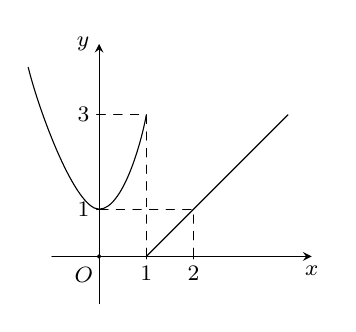
\begin{tikzpicture}[scale=0.6,font=\footnotesize,line join=round,line cap=round,>=stealth]
				\draw[->] (-1.0,0)  -- (4.5,0) node[below] {$x$};
				\foreach  \x in {1,2}
					{ 
				\draw (\x,-.05) -- (\x,.05); 
				 \draw (\x,0) node[below] {$\x$};}
				\draw[->] (0,-1.0) -- (0,4.5) node[left] {$y$}; 
				\foreach  \y in {1,3}
					{ 
				\draw (-.05,\y) -- (.05,\y); 
				\draw (0,\y) node[left]{$\y$}; 
				 }
				\draw 
					 (-1.5,4).. controls +(-76:1)
					and  +(180:.5)..(0,1).. controls +(0:.5)
					and +(-100:.6).. (1,3); 
				 \draw (1,0)--(4,3);
				\draw[dashed]  (1,0)|-(0,3)
					 (2,0)|-(0,1);
				\foreach \p/\q/\n/\g in {0/0/O/-130}\draw[fill] (\p,\q) circle (1pt)  node[shift={(\g:.3)}]{$\n$};
			\end{tikzpicture}
		 }
	\loigiai{ 
		 Dựa vào đồ thị của hàm số, ta thấy hàm số gián đoạn tại điểm có hoành độ bằng $1$.
	} 
\end{ex}

% nguồn: Ok_TracNghiemLop11_Lan1
\begin{ex}%[1D3N3-3]%[ma:5898302e]
	Cho hàm số $f\left( x \right)=\dfrac{2x-1}{{{x}^{3}}-x}$. Khẳng định  nào sau đây là đúng?
	 \choice
		 {Hàm số liên tục tại $x=-1$}
		 {Hàm số liên tục tại $x=0$}
		{Hàm số liên tục tại $x=1$} 
		{\True Hàm số liên  tục tại $x=\dfrac{1}{2}$}
	\loigiai{ 
		 Ta có $\lim\limits_{x\to\frac{1}{2}}\dfrac{2x-1}{x^{3}-x}=0$.\\
		$f\left(\dfrac{1}{2}\right)=0$.\\ 
		Vì $\lim\limits_{x\to\frac{1}{2}}\dfrac{2x-1}{x^{3}-x}=f\left(\dfrac{1}{2}\right)$ 
		nên hàm số  đã cho liên tục tại $x=\dfrac{1}{2}$.
	 }
\end{ex}

% nguồn: Ok_TracNghiemLop11_Lan1
\begin{ex}%[1D3N3-3]%[ma:8a07e5ae]
	Cho hàm  số $f(x)=\heva{&
	- x^2 + 2 x -  3 \text{ khi } x \ge -5 \\
	& - 2 x - 53 ~~\quad\text{ khi } x < -5 }$. Khẳng  định nào sau đây đúng?
	 \choice
		 { Hàm số liên tục tại mọi $x\in \mathbb{R}$}
		{ Hàm số không  liên tục tại $x=-3$}
		{ Hàm số liên tục tại $x=-5$} 
		{ \True Hàm số  không liên tục tại $x=-5$}
	 \loigiai{
		Ta có $\lim\limits_{x \to  -5^+}f(x)=\lim\limits_{x \to -5^+}(- x^2 + 2 x - 3)=-63$,
		$\lim\limits_{x  \to -5^-}f(x)=\lim\limits_{x \to -5^-}(- 2 x - 53)=-43$.\\
		Do đó $\lim\limits_{x \to  -5^+}f(x)\ne\lim\limits_{x \to -5^-}f(x)$.\\
		Vậy  hàm số không liên tục tại $x=-5$.
	} 
\end{ex}

% nguồn: Ok_TracNghiemLop11_Lan1
\begin{ex}%[1D3N3-3]%[ma:4ce70922]
	Số điểm  gián đoạn của hàm số $f(x)=\heva{&0{,}5&\text{khi}&\quad x=-1\\&\dfrac{x(x+1)}{x^2-1}&\text{khi}&\quad x\ne -1,x\ne 1\\&1&\text{khi}&\quad x=1}$ là
	\choice 
		 {$0$}
		{\True  $1$}
		 {$2$}
		{$3$} 
	\loigiai{ 
		Ta có  $\heva{&\lim\limits_{x\to 1}f(x)=\lim\limits_{x\to 1}\dfrac{x(x+1)}{x^2-1}=\lim\limits_{x\to 1}\dfrac{x}{x-1}=+\infty\\&f(1)=1.}$\\
		Do đó hàm số gián đoạn tại $x=1$.\\ 
		Mặt khác $\heva{&\lim\limits_{x\to  -1}f(x)=\lim\limits_{x\to -1}\dfrac{x(x+1)}{x^2-1}=\lim\limits_{x\to -1}\dfrac{x}{x-1}=\dfrac{1}{2}\\&f(-1)=0{,}5.}$\\
		Do đó hàm số liên tục tại  $x=-1$.\\
		Vậy hàm  số có $1$ điểm gián đoạn.
	} 
\end{ex}

% nguồn: Ok_TracNghiemLop11_Lan1
\begin{ex}%[1D3N3-3]%[ma:0f980f91]
	Cho hàm số $f(x)=\heva{&3 x+2 & \text{khi } x<-1 \\& x^2-1 & \text{khi } x \geq-1}$. Khẳng định nào sau đây  đúng?
	 \choice
		{$f(x)$  liên tục trên $\mathbb{R}$}
		{$f(x)$ liên tục trên $(-\infty;-1]$} 
		 {\True $f(x)$ liên tục trên $[-1;+\infty)$}
		 {$f(x)$ liên tục tại $x=-1$}
	 \loigiai{
		Hàm số xác định trên  $\mathbb{R}$.\\
		Ta có $f(-1)=0; \lim\limits_{x \to-1^{+}} f(x)=\lim\limits_{x \to-1^{+}}\left(x^2-1\right)=0, \lim\limits_{x \to-1^{-}}  f(x)=\lim\limits_{x \to-1^{-}}(3 x+2)=-1$.\\
		Suy ra  $f(-1)=\lim\limits_{x \to-1^{+}} f(x) \neq \lim\limits_{x \to-1^{-}} f(x)$.\\
		Vậy  hàm số đã cho liên tục trên nửa khoảng $[-1;+\infty)$ và khoảng $(-\infty;-1)$.
	 }
\end{ex}

% nguồn: Ok_Toan11_TracNghiem_Lan2
\begin{ex}%[1D3H3-3]%[ma:b2d58c94]
	Gọi $a$ là giá trị để hàm số $f(x)=\heva{& \dfrac{\sqrt{4-x}-x-2\sqrt{1+x}}{x} &\quad& \text{ khi } 0<x\le 4 \\ & a+\dfrac{4-x}{x-2} &\quad& \text{ khi } x\le 0}$ liên tục tại $x=0$. Khẳng định nào sau  đây đúng?
	 \choice
		 {$a\in \left(\dfrac{3}{5};\dfrac{4}{5}\right)$}
		{$a\in  \left(-1;-\dfrac{3}{5}\right)$}
		 {$a\in \left(0;\dfrac{2}{5}\right)$}
		{\True $a\in  \left(-\dfrac{2}{5};0\right)$}
	\loigiai{ 
		\begin{itemize}
			\item Xét $\lim\limits_{x\to 0^+}f(x)$ 
			\begin{eqnarray*}
				\lim\limits_{x\to  0^+}f(x) &=& \lim\limits_{x\to 0^+}\dfrac{\sqrt{4-x}-x-2\sqrt{1+x}}{x}\\
				&=& \lim\limits_{x\to 0^+}\left(\dfrac{\sqrt{4-x}-2\sqrt{1+x}}{x}-1\right)\\ 
				&=& \lim\limits_{x\to  0^+}\left(\dfrac{4-x-4-4x}{x\left(\sqrt{4-x}+2\sqrt{1+x}\right)}-1\right)\\
				&=& \lim\limits_{x\to 0^+}\left(\dfrac{-5x}{x(\sqrt{4-x}+2\sqrt{1+x})}-1\right)\\ 
				&=& \lim\limits_{x\to 0^+}\left(\dfrac{-5}{\sqrt{4-x}+2\sqrt{1+x}}-1\right)=-\dfrac{9}{4}. 
			\end{eqnarray*}
			\item Xét $\lim\limits_{x\to 0^-}f(x)=\lim\limits_{x\to  0^-}(a+\dfrac{4-x}{x-2})=a-2$.
			\item $f(0)=a-2$. 
		\end{itemize}
		Hàm số liên lục tại $x=0$  khi và chỉ khi
		$$\lim\limits_{x\to 0^+}f(x)=\lim\limits_{x\to 0^-}f(x)=f(0)\Leftrightarrow a-2=-\dfrac{9}{4}\Leftrightarrow a=-\dfrac{1}{4}.$$ 
		Vậy  $a\in \left(-\dfrac{2}{5};0\right)$.
	 }
\end{ex}

% nguồn: Ok_Toan11_TracNghiem_Lan2
\begin{ex}%[1D3H3-3]%[ma:b03dbebe]
	Cho hàm số $f(x)=\heva{&\dfrac{\sqrt{x+3}-2}{x-1}&\text{khi \,}x > 1\\&m^2+m+\dfrac{1}{4}&\text{khi \,}x\le 1}$. Tìm tất cả các giá trị của tham số thực $m$ để  hàm số $f(x)$ liên tục tại $x=1$.
	 \choice
		 {$m\in\{0;1\}$}
		{\True $m\in\{0;-1\}$} 
		{$m\in\{1\}$} 
		{$m\in\{0\}$} 
	\loigiai{Tập xác định  $\mathscr{D}=[-3;+\infty)$.\\
		Ta  có
		\begin{itemize}
			\item $\lim\limits_{x\to 1^+}f(x)=\lim\limits_{x\to 1^+}\dfrac{\sqrt{x+3}-2}{x-1}=\lim\limits_{x\to 1^+}\dfrac{x+3-4}{(x-1)(\sqrt{x+3}+2)}=\dfrac{1}{4}$. 
			\item $f(1)=m^2+m+\dfrac{1}{4}$. 
			\item  $\lim\limits_{x\to 1^-}f(x)=m^2+m+\dfrac{1}{4}$.
		\end{itemize}
		Để hàm số $f(x)$ liên tục tại  $x=1$ thì
		\begin{align*}
			m^2+m+\dfrac{1}{4}=\dfrac{1}{4}\Leftrightarrow m^2+m=0\Leftrightarrow m(m+1)=0\Leftrightarrow \hoac{& m=0\\&m=-1.} 
		\end{align*}
	} 
\end{ex}

% nguồn: Ok_Toan11_TracNghiem_Lan2
\begin{ex}%[1D3H3-3]%[ma:4c45b4ad]
	Tìm tất cả các giá trị  của $m$ để hàm số $f(x)=\heva{&\dfrac{\sqrt{1-x}-\sqrt{1+x}}{x}&\text{khi \,}x < 0\\&m+\sqrt{1-x}&\text{khi \,}x\ge 0}$ liên tục tại $x=0$.
	 \choice
		 {$m=1$}
		{\True $m=-2$} 
		{$m=-1$} 
		 {$m=0$}
	\loigiai{Tập xác  định $\mathscr{D}=[-1;1]$.\\
		 Ta có
		\begin{itemize}
			\item $\lim\limits_{x\to  0^-}f(x)=\lim\limits_{x\to 0^-}\dfrac{\sqrt{1-x}-\sqrt{1+x}}{x}=\lim\limits_{x\to 0^-}\dfrac{-2x}{x(\sqrt{1-x}+\sqrt{1+x})}=\dfrac{-2}{1+1}=-1$.
			\item  $\lim\limits_{x\to 0^+}f(x)=\lim\limits_{x\to 0^+}(m+\sqrt{1-x})=m+1$.
			 \item $f(0)=m+1$.
		\end{itemize}
		Để hàm số liên tục tại  $x=0$ thì $\lim\limits_{x\to 0^-}f(x)=\lim\limits_{x\to 0^+}f(x)=f(0)\Leftrightarrow-1=m+1\Leftrightarrow m=-2$.
	 }
\end{ex}

% nguồn: Ok_Toan11_TracNghiem_Lan2
\begin{ex}%[1D3H3-3]%[ma:c3768634]
	Tìm  giá trị của tham số $m$ để hàm số $f(x)=\heva{&\dfrac{\sqrt{3x+1}-2}{x-1}&\text{khi \,}x\ne 1\\&m &\text{khi \,}x=1}$ liên tục tại điểm $x=1$.
	 \choice
		{$m=3$} 
		 {$m=1$}
		{\True  $m=\dfrac{3}{4}$}
		{$m=\dfrac{1}{2}$} 
	\loigiai{Tập xác  định $\mathscr{D}=\left[-\dfrac{1}{3};+\infty\right)$.\\
		Ta có 
		\begin{itemize}
			 \item $\lim\limits_{x\to 1}\dfrac{\sqrt{3x+1}-2}{x-1}=\lim\limits_{x\to 1}\dfrac{3(x-1)}{(x-1)(\sqrt{3x+1}+2)}=\lim\limits_{x\to 1}\dfrac{3}{\sqrt{3x+1}+2}=\dfrac{3}{4}$.
			\item $f(1)=m$. 
		\end{itemize}
		Hàm số liên tục tại  $x=1$ khi và chỉ khi $m=\dfrac{3}{4}$.
	 }
\end{ex}

% nguồn: Ok_Toan11_TracNghiem_Lan2
\begin{ex}%[1D3H3-3]%[ma:94638b71]
	Hàm số nào dưới đây gián đoạn tại  điểm $x_0=2$?
	\choice 
		{$y=(x-1)(x-2)$} 
		{\True $y=\dfrac{(x-2)(x^2+3)}{x-2}$} 
		{$y=\dfrac{x-2}{x+2}$} 
		{$y=\dfrac{x+2}{x^2+2}$} 
	\loigiai{ 
		Hàm số  gián đoạn tại điểm $x_0=2$ là $y=\dfrac{(x-2)(x^2+3)}{x-2}$ vì hàm số có tập xác định $\mathscr{D}=\mathbb{R}\setminus\{2\}$.
	} 
\end{ex}

% nguồn: Ok_Toan11_TracNghiem_Lan2
\begin{ex}%[1D3H3-3]%[ma:edae9b1d]
	Cho hàm  số $f(x)=\heva{& \dfrac{x-2}{\sqrt{x+2}-2} &\quad& \text{ khi } x\ne 2 \\ & 4 &\quad& \text{ khi } x=2}$. Chọn mệnh đề đúng?
	 \choice
		{\True Hàm số liên  tục tại $x=2$}
		 {Hàm số gián đoạn tại $x=2$}
		 {$f(4)=2$}
		{$\lim\limits_{x\to 2}f(x)=2$} 
	\loigiai{ 
		Tập  xác định $\mathscr{D}=\mathbb{R}$.\\
		Ta có 
		\begin{itemize}
			\item $\lim\limits_{x\to 2}f(x)=\lim\limits_{x\to  2}\dfrac{x-2}{\sqrt{x+2}-2}=\lim\limits_{x\to 2}\dfrac{(x-2)\left(\sqrt{x+2}+2\right)}{x-2}=\lim\limits_{x\to 2}(\sqrt{x+2}+2)=4$;
			 \item $f(2)=4$.
		\end{itemize}
		Do đó $\lim\limits_{x\to  2}f(x)=f(2) \Rightarrow$ hàm số liên tục tại $x=2$.
	 }
\end{ex}

% nguồn: Ok_Toan11_TracNghiem_Lan2
\begin{ex}%[1D3H3-3]%[ma:348e4f13]
	Cho  hàm số $f(x)=\heva{&\dfrac{x^2-3x+2}{x-2}&\text{khi }x\ne 2\\
	&m&\text{khi }x=2}$. Giá trị của $m$ để hàm số $f(x)$ liên  tục tại $x=2$ là
	 \choice
		{$m=3$} 
		{\True $m=1$} 
		 {$m=-1$}
		{$m=0$} 
	\loigiai{ 
		Ta có $f(2)=m$ và  $\lim\limits_{x\to 2}f(x)=\lim\limits_{x\to 2}\dfrac{x^2-3x+2}{x-2}=\lim\limits_{x\to 2}(x-1)=1$.\\
		Vậy giá trị của $m$ để hàm số $f(x)$ liên  tục tại $x=2$ là $m=1$.
	 }
\end{ex}

% nguồn: Ok_Toan11_TracNghiem_Lan2
\begin{ex}%[1D3H3-3]%[ma:a435c469]
	Hàm  số nào dưới đây gián đoạn tại điểm $x_0=-1$?
	 \choice
		{$y=\left( x+1 \right)\left( x^2+2 \right)$} 
		{\True  $y=\dfrac{2x-3}{x+1}$}
		{$y=\dfrac{x+1}{x-1}$} 
		{$y=\dfrac{x+1}{x^2+1}$} 
	\loigiai{ 
		 Ta có $y=\dfrac{2x-1}{x+1}$ không xác định tại $x_0=-1$ nên hàm số gián đoạn tại $x_0=-1$.
	} 
\end{ex}

% nguồn: Ok_Toan11_TracNghiem_Lan2
\begin{ex}%[1D3H3-3]%[ma:2dcf933f]
	Tìm $m$ để hàm số $f(x)=\heva{& \dfrac{x^2-3x+2}{x-1} &\quad&  \text{ khi } x\ne 1 \\ & 2mx+m^2-4 &\quad& \text{ khi } x=1}$ liên tục tại $x=1$.
	\choice 
		{$m=1$} 
		{\True $\hoac{&  m=-3 \\ & m=1}$}
		{$\hoac{& m=3 \\ &  m=1}$}
		 {$m=-3$}
	\loigiai{ 
		Ta có 
		\begin{itemize}
			\item $\lim\limits_{x\to 1}f(x)=\lim\limits_{x\to 1}\dfrac{x^2-3x+2}{x-1}=\lim\limits_{x\to 1}(x-2)=-1$. 
			\item $f(1)=m^2+2m-4$. 
		\end{itemize}
		Hàm số liên tục tại  $x=1$
		$$\Leftrightarrow  \lim\limits_{x\to 1}f(x)=f(1)\Leftrightarrow m^2+2m-4=-1\Leftrightarrow \hoac{& m=1 \\ & m=-3.}$$
	} 
\end{ex}

% nguồn: Ok_Toan11_TracNghiem_Lan2
\begin{ex}%[1D3H3-3]%[ma:71b4c69c]
	Cho hàm số $f(x)=\heva{&\dfrac{x^2-3x+2}{\sqrt{x+2}-2}&\text{khi  }x>2\\
	&m^2x-4m+6&\text{khi }x\leq 2}$, $m$ là tham số. Có bao nhiêu giá trị của $m$ để hàm số đã cho  liên tục tại $x=2$?
	 \choice
		{$3$} 
		 {$0$}
		{$2$} 
		{\True  $1$}
	\loigiai{ 
		Ta có \begin{itemize}
		 \item
		$\begin{aligned}
		\lim\limits_{x\to  2^+}f(x)&=\lim\limits_{x\to 2^+}\dfrac{x^2-3x+2}{\sqrt{x+2}-2}=\lim\limits_{x\to 2^+}\dfrac{(x-2)(x-1)\left(\sqrt{x+2}+2\right)}{x-2}\\
		&=\lim\limits_{x\to  2^+}(x-1)\left(\sqrt{x+2}+2\right)=4.
	\end{aligned}$
	\item $\lim\limits_{x\to 2^-}f(x)=\lim\limits_{x\to  2^-}(m^2x-4m+6)=2m^2-4m+6$.
	\item $f(2)=2m^2-4m+6$. 
	\end{itemize}
	Hàm số  liên tục tại $x=2$ khi và chỉ khi
	\begin{eqnarray*}
		& & \lim\limits_{x\to 2^-}f(x)=\lim\limits_{x\to 2^+}f(x)=f(2)\\ 
		&\Leftrightarrow &  2m^2-4m+6=4\\
		&\Leftrightarrow & 2m^2-4m+2=0\\ 
		&\Leftrightarrow &  m=1.
	\end{eqnarray*}
	Vậy có một giá trị của $m$ thỏa mãn hàm số  đã cho liên tục tại $x=2$.
 }
\end{ex}

% nguồn: Ok_Toan11_TracNghiem_Lan2
\begin{ex}%[1D3H3-3]%[ma:76868847]
	Biết hàm số  $f(x)=
	 \heva{
	&ax^2+bx-5&\text{khi  }x\leq 1\\
	&2ax-3b&\text{khi }x>1 
	}$ liên tục tại $x=1$. Tính giá trị của  biểu thức $P=a-4b$.
	\choice 
		 {$P=-4$}
		 {$P=5$}
		 {\True $P=-5$}
		 {$P=4$}
	\loigiai{ 
		Ta có $\lim\limits_{x\to 1^-}f(x)=\lim\limits_{x\to 1^-}(ax^2+bx-5)=a+b-5=f(1)$  và
		 $\lim\limits_{x\to 1^+}f(x)=\lim\limits_{x\to 1^+}(2ax-3b)=2a-3b$.\\
		Do  hàm số liên tục tại $x=1$ nên $a+b-5=2a-3b\Rightarrow a-4b=-5$.
	} 
\end{ex}

% nguồn: Ok_Toan11_TracNghiem_Lan2
\begin{ex}%[1D3H3-3]%[ma:b9cbc88f]
	Cho hàm  số $f(x)=
	\heva{ 
	&\dfrac{3-x}{\sqrt{x+1}-2}&\text{khi  }x\ne 3\\
	 &m&\text{khi }x=3
	}$. Hàm số đã  cho liên tục tại $x=3$ khi $m$ bằng
	\choice 
		 {$-1$}
		 {$1$}
		 {$4$}
		{\True $-4$} 
	 \loigiai{
		Ta có  $f(3)=m$ và
		$\lim\limits_{x\to 3}f(x)=\lim\limits_{x\to 3}\dfrac{3-x}{\sqrt{x+1}-2}=\lim\limits_{x\to 3}\dfrac{(3-x)(\sqrt{x+1}+2)}{x-3}=\lim\limits_{x\to  3}(-\sqrt{x+1}-2)=-4$.\\
		Để hàm số liên tục tại $x=3$  thì $\lim\limits_{x\to 3}f(x)=f(3)$.\\
		Suy ra $m=-4$. 
	} 
\end{ex}

% nguồn: Ok_Toan11_TracNghiem_Lan2
\begin{ex}%[1D3H3-3]%[ma:edd89928]
	Cho hàm số $f(x)=\heva{& 3x-2 &\quad& \text{ khi } x>1 \\ & -x^2+1 &\quad& \text{  khi } x\le 1}$. Khẳng định nào sau đây đúng?
	\choice 
		{\True Hàm số gián đoạn tại $x=1$} 
		{Hàm  số liên tục tại $x=1$}
		 {Hàm số gián đoạn trên $\mathbb{R}$}
		{Hàm số liên tục  trên khoảng $(0;3)$}
	\loigiai{ 
		Ta  có
		\begin{itemize}
			\item  $\lim\limits_{x\to 1^+}f(x)=\lim\limits_{x\to 1^+}(3x-2)=1$;
			\item  $\lim\limits_{x\to 1^-}f(x)=\lim\limits_{x\to 1^-}(-x^2+1)=0$.
		\end{itemize}
		Suy ra $\lim\limits_{x\to 1^+}f(x) \ne \lim\limits_{x\to 1^-}f(x)$  nên không tồn tại $\lim\limits_{x\to 1}f(x)$.\\
		Vậy hàm số  gián đoạn tại $x=1$.
	 }
\end{ex}

% nguồn: Ok_Toan11_TracNghiem_Lan2
\begin{ex}%[1D3H3-3]%[ma:7cca53aa]
	 Tìm $a$ để hàm số $f(x)=\heva{&\dfrac{\sqrt{x+2}-2}{x-2}&\text{khi }x\ne 2\\
	 &2x+a&\text{khi }x=2}$ liên tục tại $x=2$?
	 \choice
		{$\dfrac{15}{4}$} 
		{\True $-\dfrac{15}{4}$} 
		{$\dfrac{1}{4}$} 
		 {$1$}
	 \loigiai{
		 Ta có $f(2)=4+a$.\\
		Ta tính được  $\lim\limits_{x\to 2}f(x)=\lim\limits_{x\to 2}\dfrac{\sqrt{x+2}-2}{x-2}=\lim\limits_{x\to 2}\dfrac{1}{\sqrt{x+2}+2}=\dfrac{1}{4}$.\\
		Hàm số đã cho liên tục tại $x=2$ khi và chỉ khi  $f(2)=\lim\limits_{x\to 2}f(x)\Leftrightarrow 4+a=\dfrac{1}{4}\Leftrightarrow a=-\dfrac{15}{4}$.\\
		Vậy hàm số  liên tục tại $x=2$ khi $a=-\dfrac{15}{4}$.
	} 
\end{ex}

% nguồn: Ok_Toan11_TracNghiem_Lan2
\begin{ex}%[1D3H3-3]%[ma:43ccb1c3]
	Cho hàm số $f(x)=\heva{& m^2+mx-2 &\quad& \text{ khi } x\ne 1 \\ & 0 &\quad& \text{ khi } x=1}$. Tính  tổng các giá trị của tham số $m$ để hàm số liên tuc tại $x=1$.
	\choice 
		{$2$} 
		{$4$} 
		 {$1$}
		 {\True $-1$}
	\loigiai{ 
		\begin{itemize}
			\item  $\lim\limits_{x\to 1}f(x)= \lim\limits_{x\to 1}(m^2+mx-2)=m^2+m-2$.
			\item  $f(1)=0$.
		\end{itemize}
		Hàm số  liên tục tại $x=1$
		$$\Leftrightarrow \lim\limits_{x\to 1}f(x)=f(1)\Leftrightarrow m^2+m-2=0 \Leftrightarrow  \hoac{&m=1\\ &m=-2.}$$
		Vậy tổng các giá trị của tham số $m$  cần tìm bằng $-1$.
	 }
\end{ex}

% nguồn: Ok_Toan11_TracNghiem_Lan2
\begin{ex}%[1D3H3-3]%[ma:4e218320]
	Cho hàm số $f(x)=\heva{&2x^2-1& \text{ khi } x < 0\\ &1& \text{ khi }  x=0\\ &x+1& \text{ khi } x > 0}$. Mệnh đề nào sau đây \textbf{đúng}?
	 \choice
		{\True Hàm số đã cho gián đoạn tại $x=0$} 
		{$\lim\limits_{x  \to 0}f(x)=f(0)=1$}
		 {Hàm số đã cho liên tục tại $x=0$}
		{Hàm số đã cho gián  đoạn tại $x=1$}
	\loigiai{ 
		Tập xác định  $\mathscr{D}=\mathbb{R}$.\\
		Ta có  $\lim\limits_{x \to 0^-}f(x)=\lim\limits_{x \to 0^-}(2x^2-1)=-1\neq f(0)$ và $\lim\limits_{x \to 0^+}f(x)=\lim\limits_{x \to 0^+}(x+1)=1=f(0)$.\\
		Do đó hàm  số $f$ gián đoạn tại $x=0$.
	 }
\end{ex}

% nguồn: Ok_Toan11_TracNghiem_Lan2
\begin{ex}%[1D3H3-3]%[ma:ef214313]
	 Cho hàm số $y=\dfrac{x-3}{x^2-1}$. Mệnh đề nào sau đây đúng?
	\choice 
		{\True Hàm số không liên tục tại các điểm $x=\pm 1$} 
		{Hàm số liên  tục tại mọi $x\in \mathbb{R}$}
		{Hàm số liên tục tại điểm  $x=-1$}
		{Hàm số liên tục  tại điểm $x=1$}
	 \loigiai{
		Hàm số $y=\dfrac{x-3}{x^2-1}$ có tập xác định $\mathbb{R}\setminus \left\{ \pm 1 \right\}$.\\ 
		Do  đó hàm số không liên tục tại các điểm $x=\pm 1$.
	 }
\end{ex}

% nguồn: Ok_Toan11_TracNghiem_Lan2
\begin{ex}%[1D3H3-3]%[ma:9f264c2d]
	Cho hàm số $f(x)=\heva{&\dfrac{x^2+x-2}{x-1}&\text{khi \,}x\ne 1\\&3m &\text{khi \,}x=1}$. Tìm tất cả các giá trị thực của tham số $m$ để hàm  số gián đoạn tại $x=1$.
	\choice 
		{$m\ne 2$} 
		 {\True $m\ne 1$}
		 {$m\ne-2$}
		 {$m\ne 3$}
	\loigiai{ 
		Tập xác  định $\mathscr{D}=\mathbb{R}$.\\
		Hàm số gián đoạn tại $x=1$ khi và chỉ  khi
		\begin{align*}
			\lim\limits_{x\to 1}f(x)\ne  f(1)\Leftrightarrow
			\lim\limits_{x\to  1}\dfrac{x^2+x-2}{x-1}\ne 3m\Leftrightarrow\lim\limits_{x\to 1}(x+2)\ne 3m\Leftrightarrow3\ne 3m\Leftrightarrow m\ne 1.
		\end{align*}
	 }
\end{ex}

% nguồn: Ok_Toan11_TracNghiem_Lan2
\begin{ex}%[1D3H3-3]%[ma:24d7d5a3]
	Cho hàm số $f(x)=\heva{& \dfrac{\sqrt{1+2x}-1}{x} &\quad& \text{ khi } x>0 \\ & x+2\,023 &\quad& \text{ khi }  x\le 0}$. Mệnh đề nào sau đây là đúng?
	 \choice
		{Hàm số liên tục trên  $\mathbb{R}$}
		{Hàm số  liên tục tại $x=3$}
		{\True Hàm số  gián đoạn tại $x=0$}
		 {Hàm số gián đoạn tại $x=1$}
	\loigiai{ 
		Ta có 
		\begin{itemize}
			\item $\lim\limits_{x\to 0^+}f(x)=\lim\limits_{x\to  0^+}\dfrac{\sqrt{1+2x}-1}{x}=\lim\limits_{x\to 0^+}\dfrac{2}{\sqrt{1+2x}+1}=1$.
			\item $\lim\limits_{x\to 0^-}f(x)=\lim\limits_{x\to 0^-}(x+2\,023)=2\,023$. 
		\end{itemize}
		Suy ra $\lim\limits_{x\to 0^+}f(x) \ne \lim\limits_{x\to 0^-}f(x)$.\\ 
		Do đó, không  tồn tại $\lim\limits_{x\to 0}f(x)$ nên hàm số gián đoạn tại $x=0$.
	 }
\end{ex}

% nguồn: Ok_Toan11_TracNghiem_Lan2
\begin{ex}%[1D3H3-3]%[ma:5d4bb9f2]
	Cho hàm số $y=\heva{ 
	 & \dfrac{1-x^3}{1-x},&&\text{khi }x< 1 \\
	& 1,&&\text{khi  }x\ge 1 \\
	}$. Hãy  chọn kết luận đúng trong các kết luận dưới đây?
	\choice 
		{\True Hàm số $y$ liên tục phải tại $x=1$} 
		 {Hàm số $y$ liên tục tại $x=1$}
		{hàm  số $y$ liên tục trái tại $x=1$}
		 {Hàm số $y$ liên tục trên $\mathbb{R}$}
	 \loigiai{
		Hàm số $y$ có tập xác định  là $\mathscr{D}=\mathbb{R}$.\\
		Ta có $y\left( 1  \right)=1$.\\
		Ta có $\lim\limits_{x \to 1^+}y=1$; $\lim\limits_{x \to 1^-}y=\lim\limits_{x \to 1^-} \dfrac{1-x^3}{1-x}=\lim\limits_{x \to 1^-} \dfrac{\left( 1-x \right)\left(  1+x+x^2 \right)}{1-x}=\lim\limits_{x \to 1^-}\left( 1+x+x^2 \right)=4$.\\
		Nhận thấy $\lim\limits_{x \to 1^+}y=y\left( 1 \right)$. Suy ra hàm số $y$ liên tục phải tại $x=1$. 
	} 
\end{ex}

% nguồn: Ok_Toan11_TracNghiem_Lan2
\begin{ex}%[1D3H3-3]%[ma:eae86d13]
	 Cho hàm số $f(x)=\heva{&\dfrac{x^2-3x+2}{x-2}&\text{khi \,}x\ne 2\\&a &\text{khi \,}x=2}$. Hàm số liên tục tại $x=2$ khi $a$ bằng
	\choice 
		{\True  $1$}
		 {$0$}
		{$2$} 
		 {$-1$}
	 \loigiai{Tập xác định $\mathscr{D}=\mathbb{R}$.\\
		Ta  có
		\begin{itemize}
			\item  $f(2)=a$
			\item $\lim\limits_{x\to 2}f(x)=\lim\limits_{x\to  2}\dfrac{x^2-3x+2}{x-2}=\lim\limits_{x\to 2}(x-1)=1$.
		\end{itemize}
		Hàm số liên tục  tại $x=2$ khi và chỉ khi $\lim\limits_{x\to 2}f(x)=f(2)\Leftrightarrow a=1$.\\
		Vậy  $a=1$.
	} 
\end{ex}

% nguồn: Ok_Toan11_TracNghiem_Lan2
\begin{ex}%[1D3H3-3]%[ma:d147887f]
	 Cho hàm số $y=f(x)=\heva{&\dfrac{x^3-1}{x-1}&\text{khi }x\ne 1\\
	&2m+1&\text{khi }x=1}$. Giá trị của tham  số $m$ để hàm số liên tục tại điểm $x_0=1$ là
	 \choice
		 {$m=-\dfrac{1}{2}$}
		{$m=2$} 
		{\True $m=1$} 
		 {$m=0$}
	\loigiai{ 
		Ta có $f(1)=2m+1$ và 
		$\lim\limits_{x\to 1}y=\lim\limits_{x\to 1}\dfrac{x^3-1}{x-1}=\lim\limits_{x\to 1}(x^2+x+1)=3$.\\ 
		Để hàm số liên  tục tại điểm $x_0=1$ thì $f(1)=\lim\limits_{x\to 1}y \Leftrightarrow 2m+1=3 \Rightarrow m=1$.
	} 
\end{ex}

% nguồn: Ok_Toan11_TracNghiem_Lan2
\begin{ex}%[1D3H3-3]%[ma:77ede8cb]
	Cho hàm số $f(x)=\heva{& \dfrac{\sqrt[3]{x}-1}{x-1} &\quad& \text{ khi } x\ne 1 \\ & \dfrac{2}{3} &\quad& \text{ khi } x=1}$. Khẳng  định nào sau đây là đúng?
	 \choice
		{Hàm số  liên tục tại $x=1$}
		{Hàm  số liên tục tại mọi điểm}
		{\True Hàm số gián đoạn tại tại $x=1$} 
		 {Tất cả đều sai}
	 \loigiai{
		\begin{itemize}
			\item $\lim\limits_{x\to 1}f(x)=\lim\limits_{x\to 1}\dfrac{\sqrt[3]{x}-1}{x-1}=\lim\limits_{x\to 1}\dfrac{1}{\sqrt[3]{x^2}+\sqrt[3]{x}+1}=\dfrac{1}{3}$; 
			\item $f(2)=\dfrac{2}{3}$. 
		\end{itemize}
		Do đó, hàm số gián đoạn  tại $x=1$.
	} 
\end{ex}

% nguồn: Ok_Toan11_TracNghiem_Lan2
\begin{ex}%[1D3H3-3]%[ma:e43ab11b]
	Tìm $m$ để hàm số $f(x)=\heva{&\dfrac{x^2-16}{x-4}&\text{khi \,}x > 4\\&mx+1&\text{khi \,}x\le 4}$ liên tục tại điểm  $x=4$.
	\choice 
		 {\True $m=\dfrac{7}{4}$}
		{$m=8$} 
		 {$m=-\dfrac{7}{4}$}
		 {$m=-8$}
	\loigiai{Tập xác định $\mathscr{D}=\mathbb{R}$.\\ 
		Ta  có
		\begin{itemize}
			\item  $\lim\limits_{x\to 4^+}f(x)=\lim\limits_{x\to 4^+}\dfrac{x^2-16}{x-4}=\lim\limits_{x\to 4^+}(x+4)=8$.
			\item $\lim\limits_{x\to 4^-}f(x)=\lim\limits_{x\to  4^-}(mx+1)=4m+1$.
			\item $f(4)=4m+1$. 
		\end{itemize}
		Hàm số liên tục tại điểm $x=4$ khi và chỉ khi $\lim\limits_{x\to 4^-}f(x)=\lim\limits_{x\to 4^+}f(x)=f(4)\Leftrightarrow 4m+1=8$  $\Leftrightarrow m=\dfrac{7}{4}$.
	 }
\end{ex}

% nguồn: Ok_Toan11_TracNghiem_Lan2
\begin{ex}%[1D3H3-3]%[ma:8c3649b9]
	Cho hàm  số $f(x)=\heva{& \dfrac{x^3-8}{x-2} &\quad& \text{ khi } x\ne 2 \\ & mx+1 &\quad& \text{ khi } x=2}$. Tìm tất cả các giá trị của tham số thực $m$ để hàm số liên tục tại $x=2$.
	 \choice
		 {$m=\dfrac{17}{2}$}
		{$m=\dfrac{15}{2}$} 
		{$m=\dfrac{13}{2}$} 
		 {\True $m=\dfrac{11}{2}$}
	\loigiai{ 
		Hàm số $f(x)$ xác định trên $\mathbb{R}$.\\ 
		Ta có $f(2)=2m+1$ và $\lim\limits_{x\to  2}f(x)=\lim\limits_{x\to 2}\dfrac{x^3-8}{x-2}=\lim\limits_{x\to 2}(x^2+2x+4)=12$.\\
		 Để $f(x)$ liên tục tại $x=2$
		$$\Leftrightarrow \lim\limits_{x\to  2}f(x)=f(2) \Leftrightarrow 2m+1=12\Leftrightarrow m=\dfrac{11}{2}.$$
	} 
\end{ex}

% nguồn: Ok_Toan11_TracNghiem_Lan2
\begin{ex}%[1D3H3-3]%[ma:305e8b4e]
	Tìm giá trị của tham số $m$ để hàm  số $f(x)=\heva{&\dfrac{x^2+3x+2}{x^2-1}, &x<-1\\
	&mx+2, &x\geq -1}$ liên tục tại $x=-1$. 
	\choice 
		 {$m=-\dfrac{3}{2}$}
		{$m=-\dfrac{5}{2}$} 
		{$m=\dfrac{3}{2}$} 
		{\True  $m=\dfrac{5}{2}$}
	\loigiai{ 
		Ta có 
		\begin{itemize}
			\item $f(-1)=-m+2$. 
			\item  $\lim\limits_{x\to -1^+}f(x)=-m+2$.
			\item $\lim\limits_{x\to -1^-}f(x)=\lim\limits_{x\to -1^-}\dfrac{x^2+3x+2}{x^2-1}=\lim\limits_{x\to -1^-}\dfrac{(x+1)(x+2)}{(x-1)(x+1)}=\lim\limits_{x\to  -1^-}\dfrac{x+2}{x-1}=-\dfrac{1}{2}$.
		\end{itemize}
		Hàm số liên tục tại $x=-1 \Leftrightarrow f(-1)=\lim\limits_{x\to  -1^+}f(x)=\lim\limits_{x\to -1^-}f(x) \Leftrightarrow -m+2=-\dfrac{1}{2} \Leftrightarrow m=\dfrac{5}{2}$.
	 }
\end{ex}

% nguồn: Ok_Toan11_TracNghiem_Lan2
\begin{ex}%[1D3H3-3]%[ma:46fba5fa]
	Hàm số nào  sau đây không liên tục tại $x=2$?
	\choice 
		{$y=\sqrt{x+2}$} 
		 {$y=\sin x$}
		{\True  $y=\dfrac{x^2}{x-2}$}
		 {$y=x^2-3x+2$}
	 \loigiai{
		Hàm số $y=\dfrac{x^2}{x-2}$ không xác định tại  $x=2$ nên gián đoạn tại $x=2$.
	 }
\end{ex}

% nguồn: Ok_Toan11_TracNghiem_Lan2
\begin{ex}%[1D3H3-3]%[ma:0431d513]
	Cho hàm số $f(x)=\heva{&\dfrac{\sqrt{1+2x}-1}{x} & \text{ khi } x > 0\\ &x+2\,021& \text{ khi  } x \leq 0}$. Mệnh đề nào sau đây \textbf{đúng}?
	 \choice
		{Hàm số liên tục trên $\mathbb{R}$} 
		{Hàm số gián  đoạn tại $x=3$}
		{\True Hàm số gián  đoạn tại $x=0$}
		{Hàm số gián  đoạn tại $x=1$}
	 \loigiai{
		Ta  có
		\begin{itemize}
			\item $\lim\limits_{x \to 0^+}f(x)=\lim\limits_{x \to 0^+}\dfrac{\sqrt{1+2x}-1}{x}=\lim\limits_{x \to  0^+}\dfrac{2x}{x\left(\sqrt{1+2x}+1\right)}=\lim\limits_{x \to 0^+}\dfrac{2}{\sqrt{1+2x}+1}=1$.
			\item  $\lim\limits_{x \to 0^-}f(x)=\lim\limits_{x \to 0^-}(x+2\,021)=2\,021$.
		\end{itemize}
		Suy ra $\lim\limits_{x \to 0^+}f(x)\ne\lim\limits_{x \to 0^-}f(x)$ nên $\lim\limits_{x \to  0}f(x)$ không tồn tại.\\
		Vậy hàm số gián đoạn  tại $x=0$.
	 }
\end{ex}

% nguồn: Ok_Toan11_TracNghiem_Lan2
\begin{ex}%[1D3H3-3]%[ma:cfc2f9c8]
	Cho hàm số $f(x)=\heva{&x^2+2& \text{  khi } x > 0\\ &x & \text{ khi } x\leq 0}$. Mệnh đề nào sau đây \textbf{sai}?
	\choice 
		 {$f(0)=0$}
		{\True $f(x)$ liên tục tại $x_0=0$} 
		 {$\lim\limits_{x \to 0^-}f(x)=0$}
		{$\lim\limits_{x  \to 0^+}f(x)=2$}
	 \loigiai{
		Ta  có
		 $\heva{
		 &f(0)=0\\
		&\lim\limits_{x \to 0^-}f(x)=\lim\limits_{x \to 0^-}x=0\\ 
		&\lim\limits_{x \to 0^+}f(x)=\lim\limits_{x \to  0^+}(x^2+2)=0^2+2=2}$.\\
		Do đó hàm số gián đoạn  tại $x_0=0$.
	 }
\end{ex}

% nguồn: Ok_Toan11_TracNghiem_Lan2
\begin{ex}%[1D3H3-3]%[ma:effb0cc9]
	Tìm $m$ để hàm số $f(x)=\heva{& \dfrac{x^2-1}{x-1} &\quad& \text{ khi } x\ne 1 \\ &  m+2 &\quad& \text{ khi } x=1}$ liên tục tại điểm $x_0=1$.
	\choice 
		{$m=3$} 
		{\True  $m=0$}
		 {$m=4$}
		{$m=1$} 
	\loigiai{ 
		 Tập xác định $\mathscr{D}=\mathbb{R}\Rightarrow x_0=1\in \mathscr{D}$.\\
		Ta có $f(1)=m+2$ và $\lim\limits_{x\to  1}\dfrac{x^2-1}{x-1}=\lim\limits_{x\to 1}\dfrac{(x+1)(x-1)}{x-1}=\lim\limits_{x\to 1}(x+1)=2$.\\
		Hàm  số $f(x)$ liên tục tại điểm $x_0=1$ khi và chỉ khi
		$$\lim\limits_{x\to 1}f(x)=f(1)\Rightarrow  m+2=2\Leftrightarrow m=0.$$
	 }
\end{ex}

% nguồn: Ok_Toan11_TracNghiem_Lan2
\begin{ex}%[1D3H3-3]%[ma:5756d636]
	Tìm giá trị của tham số $m$ để hàm  số $f(x)=\heva{& \dfrac{x^2+3x+2}{x^2-1} &\quad& \text{ khi } x<-1 \\ & mx+2 &\quad& \text{ khi } x\ge -1}$ gián đoạn tại $x=-1$.
	\choice 
		{$m=\dfrac{3}{2}$} 
		 {$m=\dfrac{5}{2}$}
		{$m\ne \dfrac{3}{2}$} 
		 {\True $m\ne \dfrac{5}{2}$}
	 \loigiai{
		Ta  có
		\begin{itemize}
			\item $\lim\limits_{x\to  -1^-}f(x)=\lim\limits_{x\to -1^-}\dfrac{x^2+3x+2}{x^2-1}=\lim\limits_{x\to -1^-}\dfrac{x+2}{x-1}=\dfrac{-1}{2}$.
			\item $\lim\limits_{x\to -1^+}f(x)=\lim\limits_{x\to  -1^+}(mx+2)=-m+2$.
			\item $f(-1)=-m+2$. 
		\end{itemize}
		 Do đó để hàm số gián đoạn tại $x=-1$ thì $-m+2\ne \dfrac{-1}{2}\Leftrightarrow m\ne \dfrac{5}{2}$.
	 }
\end{ex}

% nguồn: Ok_Toan11_TracNghiem_Lan2
\begin{ex}%[1D3H3-3]%[ma:9e133c4c]
	Biết hàm  số $f(x)=\heva{&3x+b&\text{khi }x\leq -1\\
	&x+a&\text{khi }x>-1}$ liên tục tại  $x=-1$. Mệnh đề nào dưới đây đúng?
	 \choice
		{\True $a=b-2$} 
		 {$a=-2-b$}
		 {$a=2-b$}
		 {$a=b+2$}
	\loigiai{ 
		Ta có $\lim\limits_{x\to  -1^-}f(x)=f(-1)=b-3$ và $\lim\limits_{x\to -1^+}f(x)=a-1$.\\
		Hàm số liên tục tại $x=-1 \Leftrightarrow \lim\limits_{x\to -1}f(x)=f(-1) \Leftrightarrow b-3=a-1  \Leftrightarrow a=b-2$.
	 }
\end{ex}

% nguồn: Ok_Toan11_TracNghiem_Lan2
\begin{ex}%[1D3H3-3]%[ma:0d6f7539]
	Tìm $m$, $n$ để hàm số $f(x)=\heva{& \dfrac{x^3-x^2}{x-1} &\quad& \text{ khi } x>1 \\ & n &\quad& \text{  khi } x=1 \\ & mx+1 &\quad& \text{ khi } x<1}$ liên tục tại $x=1$.
	 \choice
		{$n=-1$ và $m=0$} 
		{$n=m=1$} 
		 {$n=0$ và $m=1$}
		 {\True $n=1$ và $m=0$}
	 \loigiai{
		Tập xác định  $\mathscr{D}=\mathbb{R}$, ta có
		\begin{itemize}
			\item  $f(1)=n$.
			\item $\lim\limits_{x\to 1^+}f(x)=\lim\limits_{x\to 1^+}\dfrac{x^3-x^2}{x-1}=\lim\limits_{x\to  1^+}\dfrac{x^2(x-1)}{x-1}=\lim\limits_{x\to 1^+}{x^2}=1$.
			\item  $\lim\limits_{x\to 1^-}f(x)=\lim\limits_{x\to 1^-}(mx+1)=m+1$.
		\end{itemize}
		Hàm  số $f(x)$ liên tục tại $x=1$ khi và chỉ khi
		$$\lim\limits_{x\to 1^-}f(x)=\lim\limits_{x\to 1^+}f(x)=f(1)\Leftrightarrow m+1=n=1\Leftrightarrow  \heva{& m=0 \\ & n=1.}$$
	 }
\end{ex}

% nguồn: Ok_Toan11_TracNghiem_Lan2
\begin{ex}%[1D3H3-3]%[ma:478701ba]
	Hàm số $y=\dfrac{1}{x^2-4}$ gián đoạn tại điểm nào dưới  đây?
	 \choice
		 {$x=1$}
		 {$x=0$}
		 {\True $x=2$}
		 {$x=-1$}
	\loigiai{ 
		Hàm số $y=\dfrac{1}{x^2-4}$ không xác định  tại $x=2$ nên gián đoạn tại $x=2$.
	 }
\end{ex}

% nguồn: Ok_Toan11_TracNghiem_Lan2
\begin{ex}%[1D3H3-3]%[ma:44c780df]
	Tìm tất cả các giá trị của tham số $m$ để hàm số $f(x)=\heva{&\dfrac{x^2-2x}{x-2}&\text{khi \,}x > 2\\&mx-4&\text{khi \,}x\le 2}$ liên tục tại $x=2$. 
	\choice 
		 {\True $m=3$}
		{$m=2$} 
		{$m=-2$} 
		{Không  tồn tại $m$}
	 \loigiai{Tập xác định $\mathscr{D}=\mathbb{R}$.\\
		 Ta có
		\begin{itemize}
			\item $\lim\limits_{x\to 2^+}f(x)=\lim\limits_{x\to 2^+}\dfrac{x^2-2x}{x-2}=\lim\limits_{x\to 2^+}\dfrac{x(x-2)}{x-2}=\lim\limits_{x\to 2^+}x=2$. 
			 \item $\lim\limits_{x\to 2^-}f(x)=\lim\limits_{x\to 2^-}(mx-4)=2m-4$.
		\end{itemize}
		Hàm số liên tục tại $x=2$ khi  và chỉ khi $\lim\limits_{x\to 2^+}f(x)=\lim\limits_{x\to 2^-}f(x)=f(2)\Leftrightarrow 2m-4=2 \Leftrightarrow m=3$.
	} 
\end{ex}

% nguồn: Ok_Toan11_TracNghiem_Lan2
\begin{ex}%[1D3H3-3]%[ma:8d11927e]
	Cho hàm số $f(x)=\heva{&x^2-2x+3&\text{khi \,}x\ne 1\\&3x+m-1&\text{khi  \,}x=1}$. Tìm $m$ để hàm số liên tục tại $x=1$.
	\choice 
		{$m=1$} 
		 {$m=3$}
		{\True $m=0$} 
		{$m=2$} 
	 \loigiai{
		Tập  xác định $\mathscr{D}=\mathbb{R}$.\\
		Ta  có
		\begin{itemize}
			 \item $f(1)=2+m$.
			\item $\lim\limits_{x\to  1}f(x)=\lim\limits_{x\to 1}(x^2-2x+3)=2$.
		\end{itemize}
		Hàm số liên tục tại  $x=1$ khi và chỉ khi $\lim\limits_{x\to 1}f(x)=f(1)\Leftrightarrow 2=m+2\Leftrightarrow m=0$.
	 }
\end{ex}

% nguồn: Ok_Toan11_TracNghiem_Lan2
\begin{ex}%[1D3H3-3]%[ma:8d9e831c]
	Cho hàm số $f(x)=\heva{&\dfrac{4-x^2}{x-2} & \text{ khi } x < 2\\ &-3& \text{ khi } x=2\\ &1-2x & \text{ khi } x > 2.}$ Mệnh đề  nào sau đây \textbf{đúng}?
	 \choice
		{\True Hàm số không có giới hạn  tại $x=2$ và không liên tục tại $x=2$}
		{Hàm số có giới hạn tại $x=2$ và liên tục tại $x=2$} 
		{Hàm số không có giới hạn tại  $x=2$ nhưng liên tục tại $x=2$}
		{Hàm số có giới hạn tại $x=2$ nhưng không  liên tục tại $x=2$}
	\loigiai{ 
		Tập xác định:  $\mathscr{D}=\mathbb{R}$\\
		Ta có $\heva{ 
		&f(2)=-3\\ 
		&\lim\limits_{x \to 2^-}f(x)=\lim\limits_{x \to 2^-}\dfrac{4-x^2}{x-2}=\lim\limits_{x \to 2^-}\dfrac{-(x-2)(x+2)}{x-2}=\lim\limits_{x  \to 2^-}(-x-2)=-4\\
		&\lim\limits_{x \to 2^+}f(x)=\lim\limits_{x \to  2^+}(1-2x)=-3.
		 }$\\
		Suy ra hàm số không có giới hạn tại $x=2$ và không liên tục tại  $x=2$.
	 }
\end{ex}

% nguồn: Ok_Toan11_TracNghiem_Lan2
\begin{ex}%[1D3H3-3]%[ma:6238dca2]
	Cho hàm số $f(x)=\heva{& \dfrac{\sqrt{5x-1}-\sqrt[3]{x^2+x+6}}{1-x} &\quad&  \text{ khi } x>1 \\ & ax+2 &\quad& \text{ khi } x\le 1}$. Tìm $a$ để hàm số liên tục tại $x=1$.
	 \choice
		{\True $-3$} 
		 {$3$}
		{$-1$} 
		 {$0$}
	\loigiai{ 
		\begin{itemize}
			\item Xét $\lim\limits_{x\to  1^+}f(x)$
			\begin{eqnarray*}
				&=&  \lim\limits_{x\to 1^+}\dfrac{\sqrt{5x-1}-\sqrt[3]{x^2+x+6}}{1-x}\\
				&=& \lim\limits_{x\to 1^+}\dfrac{\sqrt{5x-1}-2+2-\sqrt[3]{x^2+x+6}}{1-x}\\ 
				&=& \lim\limits_{x\to  1^+}\left(\dfrac{\sqrt{5x-1}-2}{1-x}+\dfrac{2-\sqrt[3]{x^2+x+6}}{1-x}\right)\\
				&=& \lim\limits_{x\to 1^+}\left(\dfrac{5x-5}{(1-x)\left(\sqrt{5x-1}+2\right)}+\dfrac{8-(x^2+x+6)}{(1-x)\left(4+2\sqrt[3]{x^2+x+6}+(\sqrt[3]{x^2+x+6})^2\right)}\right)\\ 
				 &=& \lim\limits_{x\to 1^+}\left(\dfrac{-5}{\sqrt{5x-1}+2}+\dfrac{x+2}{4+2\sqrt[3]{x^2+x+6}+(\sqrt[3]{x^2+x+6})^2}\right)\\
				&=&  -\dfrac{5}{4}+\dfrac{1}{4}=-1.
			\end{eqnarray*}
			\item Xét  $\lim\limits_{x\to 1^-}f(x)=\lim\limits_{x\to 1^-}(ax+2)=a+2$.
			\item  $f(1)=a+2$.
		\end{itemize}
		Hàm số liên tục tại  $x=1$
		$$\Leftrightarrow \lim\limits_{x\to 1^+}f(x)=\lim\limits_{x\to 1^-}f(x)=f(1)\Leftrightarrow  a+2=-1\Leftrightarrow a=-3.$$
	} 
\end{ex}

% nguồn: Ok_Toan11_TracNghiem_Lan2
\begin{ex}%[1D3H3-3]%[ma:5a777998]
	Hàm số $f(x)=\heva{&x^2+1&\text{khi \,}x\le 1\\&x+m &\text{khi \,}x > 1}$ liên tục tại điểm $x=1$ khi  $m$ nhận giá trị
	\choice 
		{$m=-2$} 
		 {$m=2$}
		{$m=-1$} 
		 {\True $m=1$}
	\loigiai{Tập  xác định $\mathscr{D}=\mathbb{R}$.\\
		 Ta có
		\begin{itemize}
			\item  $\lim\limits_{x\to 1^-}f(x)=\lim\limits_{x\to 1^-}(x^2+1)=2$.
			\item  $\lim\limits_{x\to 1^+}f(x)=\lim\limits_{x\to 1^+}(x+m)=1+m$.
		\end{itemize}
		Để hàm số liên tục tại $x=1$ thì $\lim\limits_{x\to 1^-}f(x)=\lim\limits_{x\to 1^+}f(x)\Leftrightarrow  2=m+1\Leftrightarrow m=1$.
	} 
\end{ex}

% nguồn: Ok_Toan11_TracNghiem_Lan2
\begin{ex}%[1D3H3-3]%[ma:a456e167]
	Gọi $S$ là tập các giá trị của tham số $m$ để hàm số $f(x)=\heva{& x^2-3x &\quad& \text{ khi }  x\ne 1 \\ & m^2+m-8 &\quad& \text{ khi } x=1}$ liên tục tại $x=1$. Tích các phần tử của tập $S$ bằng
	\choice 
		{$-2$} 
		 {$-8$}
		{\True $-6$} 
		{$-1$} 
	 \loigiai{
		\begin{itemize}
			\item  $f(1)=m^2+m-8$.
			\item $\lim\limits_{x\to 1}f(x)=\lim\limits_{x\to 1}(x^2-3x)=-2$. 
		\end{itemize}
		Hàm số  $f(x)$ liên tục tại điểm $x=1$
		$$\Leftrightarrow  \lim\limits_{x\to 1}f(x)=f(1)\Leftrightarrow m^2+m-8=-2\Leftrightarrow \hoac{& m=2 \\ & m=-3.}$$
		Vậy $S=\left\{  2;-3 \right\}$. Tích các phần tử $S$ là $-6$.
	 }
\end{ex}

% nguồn: Ok_Toan11_TracNghiem_Lan2
\begin{ex}%[1D3H3-3]%[ma:1e15aa0c]
	Hàm số $y=\dfrac{x}{x+1}$ gián đoạn tại điểm $x_0$ bằng  bao nhiêu?
	 \choice
		 {$x_0=2\,018$}
		{$x_0=1$} 
		{$x_0=0$} 
		{\True  $x_0=-1$}
	\loigiai{ 
		Vì hàm số $y=\dfrac{x}{x+1}$ có TXĐ: $\mathscr{D}=\mathbb{R}\setminus \left\{-1 \right\}$ nên hàm số gián đoạn  tại điểm $x_0=-1$.
	 }
\end{ex}

% nguồn: Ok_Toan11_TracNghiem_Lan2
\begin{ex}%[1D3H3-3]%[ma:018bbfc8]
	Cho hàm số $f(x)=\heva{&\dfrac{x-2}{\sqrt{x+2}-2} & \text{ khi } x \neq 2\\ &4& \text{ khi } x=2}$. Mệnh đề nào sau đây  \textbf{đúng}?
	 \choice
		{\True Hàm số liên tục tại $x=2$} 
		{Hàm số gián  đoạn tại $x=2$}
		{$f(4)=2$} 
		{$\lim\limits_{x \to 2}f(x)=2$} 
	\loigiai{ 
		Tập xác định của hàm số  là $\mathscr{D}=\mathbb{R}$.\\
		 Ta có $f(2)=4$.\\
		$\lim\limits_{x \to  2}f(x)=\lim\limits_{x \to 2}\dfrac{x-2}{\sqrt{x+2}-2}=\lim\limits_{x \to 2}\dfrac{(x-2)\left(\sqrt{x+2}+2\right)}{x-2}=\lim\limits_{x \to 2}\left(\sqrt{x+2}+2\right)=\sqrt{2+2}+2=4$.\\
		Vậy hàm số  liên tục tại $x=2$.
	} 
\end{ex}

% nguồn: Ok_Toan11_TracNghiem_Lan2
\begin{ex}%[1D3H3-3]%[ma:0b5e9bad]
	Tìm các giá trị của tham số $m$ để  hàm số $f(x)=\heva{&\dfrac{x^2-3x+2}{x^2-2x}&\text{khi \,}x < 2\\&mx+m+1&\text{khi \,}x\ge 2}$ liên tục tại điểm $x=2$.
	 \choice
		 {$m=\dfrac{1}{6}$}
		{\True $m=-\dfrac{1}{6}$} 
		{$m=-\dfrac{1}{2}$} 
		{$m=\dfrac{1}{2}$} 
	\loigiai{Tập xác định $\mathscr{D}=\mathbb{R}\setminus\{0\}$.\\ 
		Ta  có
		\begin{itemize}
			\item $\lim\limits_{x\to  2^-}\dfrac{x^2-3x+2}{x^2-2x}=\lim\limits_{x\to 2^-}\dfrac{(x-2)(x-1)}{x(x-2)}=\lim\limits_{x\to 2^-}\dfrac{x-1}{x}=\dfrac{1}{2}$.
			 \item $f(2)=2m+m+1=3m+1$.
		\end{itemize}
		Để  hàm số liên tục tại điểm $x=2\Leftrightarrow 3m+1=\dfrac{1}{2}\Leftrightarrow m=-\dfrac{1}{6}$.
	 }
\end{ex}

% nguồn: Ok_Toan11_TracNghiem_Lan2
\begin{ex}%[1D3H3-3]%[ma:bd7e4ca6]
	Để hàm số  $y=\heva{&x^2+3x+2&\text{khi }x\leq -1\\
	&4x+a&\text{khi  }x>-1}$ liên tục tại điểm $x=-1$ thì giá trị của $a$ là
	 \choice
		{$-4$} 
		 {\True $4$}
		 {$1$}
		 {$-1$}
	 \loigiai{
		Hàm số liên  tục tại $x=-1$ khi và chỉ khi
		\begin{eqnarray*}
			 & & \lim\limits_{x\to -1^-}y=\lim\limits_{x\to -1^+}y=y(-1)\\
			&\Leftrightarrow & \lim\limits_{x\to -1^+}(4x+a)=\lim\limits_{x\to -1^-}(x^2+3x+2)=y(-1)\\ 
			&\Leftrightarrow  & a-4=0\\
			&\Leftrightarrow &  a=4.
		\end{eqnarray*}
	} 
\end{ex}

% nguồn: Ok_Toan11_TracNghiem_Lan2
\begin{ex}%[1D3H3-3]%[ma:6b9781e5]
	Cho hàm  số $f(x)=\heva{&\dfrac{2x^2+3x-14}{x^2-4}&\text{khi }x\ne 2\\
	 &m&\text{khi }x=2}$. Với giá trị nào của $m$ thì hàm số liên tục tại $x=2$?
	 \choice
		{$-\dfrac{11}{4}$} 
		 {$-\dfrac{11}{2}$}
		{$\dfrac{11}{2}$} 
		{\True  $\dfrac{11}{4}$}
	 \loigiai{
		Hàm số xác định với  mọi $x\in \mathbb{R}$.\\
		Ta có $\lim\limits_{x\to 2}f(x)=\lim\limits_{x\to  2}\dfrac{2x^2+3x-14}{x^2-4}=\lim\limits_{x\to 2}\dfrac{(x-2)(2x+7)}{(x-2)(x+2)}=\lim\limits_{x\to 2}\dfrac{2x+7}{x+2}=\dfrac{11}{4}$ và $f(2)=m$.\\
		Để hàm số liên tục tại $x=2$ thì $\lim\limits_{x\to 2}f(x)=f(2)\Leftrightarrow m=\dfrac{11}{4}$. 
	 }
\end{ex}

% nguồn: Ok_Toan11_TracNghiem_Lan2
\begin{ex}%[1D3H3-3]%[ma:b63ee408]
	Cho hàm số $f(x)=\heva{& -x\cos x &\quad& \text{ khi } x<0 \\ & \dfrac{x^2}{1+x} &\quad& \text{ khi } 0\le x<1 \\ & x^3 &\quad& \text{ khi } x\ge 1}$. Khẳng định nào sau  đây đúng?
	 \choice
		{Hàm số $f(x)$ liên tục tại mọi điểm  $x$ thuộc $\mathbb{R}$}
		{Hàm số $f(x)$  bị gián đoạn tại điểm $x=0$}
		{\True  Hàm số $f(x)$ bị gián đoạn tại điểm $x=1$}
		{Hàm số $f(x)$ bị gián đoạn  tại điểm $x=0$ và $x=1$}
	 \loigiai{
		Ta có 
		\begin{itemize}
			\item $\lim\limits_{x\to 0^-}f(x)=\lim\limits_{x\to  0^-}(-x\cos x)=0$.
			\item $\lim\limits_{x\to 0^+}f(x)=\lim\limits_{x\to 0^+}\dfrac{x^2}{1+x}=0$. 
			\item  $f(0)=0$.
		\end{itemize}
		Suy ra $\lim\limits_{x\to 0^-}f(x)=\lim\limits_{x\to 0^+}f(x)=f(0) \Rightarrow$ hàm số liên tục  tại $x=0$.
		\begin{itemize}
			 \item $\lim\limits_{x\to 1^-}f(x)=\lim\limits_{x\to 1^-}\dfrac{x^2}{1+x}=\dfrac{1}{2}$.
			\item  $\lim\limits_{x\to 1^+}f(x)=\lim\limits_{x\to 1^+}x^3=1$.
		\end{itemize}
		 Do đó không tồn tại $\lim\limits_{x\to 1}f(x) \Rightarrow$ hàm số gián đoạn tại $x=1$.
	} 
\end{ex}

% nguồn: Ok_Toan11_TracNghiem_Lan2
\begin{ex}%[1D3H3-3]%[ma:4a9b6727]
	Cho hàm số $f(x)=\heva{&\dfrac{x^2-1}{x-1} & \text{ khi } x \neq 1\\ &2& \text{  khi } x=1}$. Mệnh đề nào sau đây \textbf{đúng}?
	\choice 
		{$f(1)$  không tính được}
		{$\lim\limits_{x \to 1}f(x)=0$} 
		 {$f(x)$ gián đoạn tại $x=1$}
		{\True $f(x)$ liên tục tại  $x=1$}
	\loigiai{ 
		Hàm số $f(x)$  xác định trên $\mathbb{R}$\\
		 $\lim\limits_{x \to 1}f(x)=\lim\limits_{x \to 1}\dfrac{x^2-1}{x-1}=\lim\limits_{x \to 1}(x+1)=2$ và $f(1)=2$.\\
		Suy ra hàm số  đã cho liên tục tại $x=1$.
	} 
\end{ex}

% nguồn: Ok_Toan11_TracNghiem_Lan2
\begin{ex}%[1D3H3-3]%[ma:6e264672]
	Cho hàm số $f(x)=\heva{& \dfrac{x^2-4x+3}{x-1} &\quad& \text{ khi } x>1 \\ & ax+1 &\quad& \text{ khi  } x\le 1}$. Xác định số thực $a$ để hàm số liên tục tại điểm $x=1$.
	\choice 
		 {$a=-1$}
		{$a=1$} 
		{$a=3$} 
		{\True $a=-3$} 
	 \loigiai{
		Tập  xác định $\mathscr{D}=\mathbb{R}$.\\
		Ta  có
		\begin{itemize}
			\item  $f(1)=a+1$;
			\item  $\lim\limits_{x\to 1^-}f(x)=\lim\limits_{x\to 1^-}(ax+1)=a+1$;
			\item $\lim\limits_{x\to 1^+}f(x)=\lim\limits_{x\to 1^+}\dfrac{x^2-4x+3}{x-1}=\lim\limits_{x\to 1^+}(x-3)=-2.$ 
		\end{itemize}
		Hàm số đã cho liên  tục tại $x=1$ khi và chỉ khi
		$$f(1)=\lim\limits_{x\to 1^-}f(x)=\lim\limits_{x\to 1^+}f(x)\Leftrightarrow  a+1=-2\Leftrightarrow a=-3.$$
	} 
\end{ex}

% nguồn: Ok_Toan11_TracNghiem_Lan2
\begin{ex}%[1D3H3-3]%[ma:c3082b3a]
	Để hàm số $f(x)=\heva{&\dfrac{2x^2-3x+1}{2(x-1)}&\text{khi \,}x\ne 1\\&m &\text{khi \,}x=1}$ liên tục tại $x=1$ thì giá trị  $m$ bằng
	 \choice
		{\True $0{,}5$} 
		 {$1{,}5$}
		{$1$} 
		{$2$} 
	 \loigiai{Tập xác định $\mathscr{D}=\mathbb{R}$.
		\begin{itemize}
			\item $f(1)=m$. 
			\item  $\lim\limits_{x\to 1}f(x)=\lim\limits_{x\to 1}\dfrac{2x^2-3x+1}{2(x-1)}=\lim\limits_{x\to 1}\dfrac{(x-1)(2x-1)}{2(x-1)}=\lim\limits_{x\to 1}\dfrac{2x-1}{2}=\dfrac{1}{2}$.
		\end{itemize}
		Để hàm số $f(x)$ liên tục tại $x=1$ thì  $\lim\limits_{x\to 1}f(x)=f(1)\Leftrightarrow m=\dfrac{1}{2}$.
	} 
\end{ex}

% nguồn: Ok_Toan11_TracNghiem_Lan2
\begin{ex}%[1D3H3-3]%[ma:2c0e9049]
	Cho hàm số $f(x)=\heva{& \dfrac{x^2-3x+2}{x-1} &\quad& \text{ khi } x\ne 1 \\ & m &\quad& \text{ khi } x=1}$. Tìm $m$  để hàm số liên tục tại $x=1$.
	\choice 
		 {$m=-2$}
		 {$m=2$}
		 {\True $m=-1$}
		{$m=1$} 
	 \loigiai{
		Tập xác định $\mathscr{D}=\mathbb{R}$. 
		\begin{itemize}
			 \item $f(1)=m$.
			 \item $\lim\limits_{x\to 1}f(x)=\lim\limits_{x\to 1}\dfrac{x^2-3x+2}{x-1}=\lim\limits_{x\to 1}\dfrac{(x-1)(x-2)}{x-1}=\lim\limits_{x\to 1}(x-2)=1-2=-1$.
		\end{itemize}
		Hàm số liên tục tại điểm $x=1$ 
		$$\Leftrightarrow  \lim\limits_{x\to 1}f(x)=f(1)\Leftrightarrow m=-1.$$
	} 
\end{ex}

% nguồn: Ok_Toan11_TracNghiem_Lan2
\begin{ex}%[1D3H3-3]%[ma:69899cfb]
	Tìm tham số  thực $m$ để hàm số $y=f(x)=\heva{&\dfrac{x^2+x-12}{x+4}&\text{khi \,}x\ne-4\\&mx+1&\text{khi \,}x=-4}$ liên tục tại điểm $x=-4$.
	 \choice
		 {$m=4$}
		{$m=3$} 
		{\True  $m=2$}
		 {$m=5$}
	\loigiai{ 
		Tập xác định $\mathscr{D}=\mathbb{R}$.\\ 
		 Ta có
		\begin{itemize}
			\item $\lim\limits_{x\to-4}f(x)=\lim\limits_{x\to-4}\dfrac{x^2+x-12}{x+4}=\lim\limits_{x\to-4}\dfrac{(x-3)(x+4)}{x+4}=\lim\limits_{x\to-4}(x-3)=-7$. 
			\item  $f(-4)=-4m+1$.
		\end{itemize}
		Hàm số $f(x)$ liên tục tại điểm $x=-4$  khi và chỉ khi
		\begin{align*}
			\lim\limits_{x\to-4}f(x)=f(-4)\Leftrightarrow-4m+1=-7\Leftrightarrow m=2. 
		\end{align*}
	} 
\end{ex}

% nguồn: Ok_Toan11_TracNghiem_Lan2
\begin{ex}%[1D3H3-3]%[ma:3dd7c4df]
	Cho hàm số $y=f(x)=\heva{& \dfrac{\sqrt[3]{ax+1}-\sqrt{1-bx}}{x} &\quad& \text{ khi } x\ne 0 \\ & 3a-5b-1 &\quad& \text{ khi } x=0}$. Tìm điều kiện của tham số $a,b$ để hàm số trên  liên tục tại điểm $x=0$. Khẳng định nào sau đây là đúng?
	\choice 
		{$a-8b=1$} 
		 {$2a-6b=1$}
		{\True $16a-33b=6$} 
		 {$2a-4b=1$}
	 \loigiai{
		\begin{itemize}
			\item Tính $\lim\limits_{x\to 0}f(x)$. 
			\begin{eqnarray*}
				\lim\limits_{x\to 0}f(x) &=&  \lim\limits_{x\to 0}\dfrac{\sqrt[3]{ax+1}-\sqrt{1-bx}}{x}\\
				 &=& \lim\limits_{x\to 0}\dfrac{\sqrt[3]{ax+1}-1+1-\sqrt{1-bx}}{x}\\
				&=& \lim\limits_{x\to 0}\left(\dfrac{\sqrt[3]{ax+1}-1}{x}+\dfrac{1-\sqrt{1-bx}}{x}\right)\\ 
				&=& \lim\limits_{x\to 0}\left(\dfrac{ax+1-1}{x\left(\sqrt[3]{(ax+1)^2}+\sqrt[3]{ax+1}+1^2\right)}+\dfrac{1-(1-bx)}{x\left(1+\sqrt{1-bx}\right)}\right)\\ 
				&=&  \lim\limits_{x\to 0}\left(\dfrac{a}{\sqrt[3]{(ax+1)^2}+\sqrt[3]{ax+1}+1^2}+\dfrac{b}{1+\sqrt{1-bx}}\right)\\
				&=& \dfrac{a}{3}+\dfrac{b}{2}=\dfrac{2a+3b}{6}. 
			\end{eqnarray*}
			\item $f(0)=3a-5b-1$. 
		\end{itemize}
		Hàm số  liên tục tại $x=0$
		$$\Leftrightarrow \lim\limits_{x\to 0}f(x)=f(0) \Leftrightarrow \dfrac{2a+3b}{6}=3a-5b-1 \Leftrightarrow 16a-33b=6.$$ 
	} 
\end{ex}

% nguồn: Ok_Toan11_TracNghiem_Lan2
\begin{ex}%[1D3H3-3]%[ma:7eb743c1]
	 Hàm số $y=\dfrac{5}{x(x^2-1)}$ liên tục tại điểm nào sau đây?
	\choice 
		{$x=0$} 
		{\True $x=\sqrt{2}$} 
		{$x=1$} 
		 {$x=-1$}
	 \loigiai{
		Đặt  $f(x)=\dfrac{5}{x(x^2-1)}$.\\
		Hàm số $y=\dfrac{5}{x(x^2-1)}$ xác định khi $\heva{& x\ne 0  \\ & x-1\ne 0 \\ & x+1\ne 0} \Leftrightarrow \heva{& x\ne 0 \\ & x\ne 1 \\ & x\ne -1.}$\\
		 Ta thấy $\lim\limits_{x\to \sqrt{2}}\dfrac{5}{x(x^2-1)}=\dfrac{5}{\sqrt{2}(2-1)}=\dfrac{5\sqrt{2}}{2}$; $f\left(\sqrt{2}\right)=\dfrac{5\sqrt{2}}{2}$.\\
		Do  đó $\lim\limits_{x\to \sqrt{2}}\dfrac{5}{x(x^2-1)}=f\left(\sqrt{2}\right)=\dfrac{5\sqrt{2}}{2}$.\\
		Suy ra  hàm số liên tục tại $x=\sqrt{2}$.
	} 
\end{ex}

% nguồn: Ok_Toan11_TracNghiem_Lan2
\begin{ex}%[1D3H3-3]%[ma:976373e0]
	Cho hàm số $f(x)=\heva{& \dfrac{\sqrt{(x-3)^2}}{x-3} &\quad& \text{ khi } x\ne 3 \\ & m &\quad& \text{ khi } x=3}$. Tìm tất cả các giá trị của tham số  thực $m$ để hàm số liên tục tại $x=3$.
	 \choice
		{\True $m\in \varnothing$} 
		{$m\in \mathbb{R}$} 
		 {$m=1$}
		 {$m=-1$}
	 \loigiai{
		Hàm số đã cho  xác định trên $\mathscr{D}= \mathbb{R}$.
		\begin{itemize}
			\item $\lim\limits_{x \to 3^-}f(x)=  \lim\limits_{x \to 3^-}\dfrac{\sqrt{(x-3)^2}}{x-3}=\lim\limits_{x \to 3^-}\dfrac{\left| x-3 \right|}{x-3}=-1$.
			\item  $\lim\limits_{x \to 3^+}f(x)= \lim\limits_{x \to 3^+}\dfrac{\sqrt{(x-3)^2}}{x-3}=\lim\limits_{x \to 3^+}\dfrac{\left| x-3 \right|}{x-3}=1$.
		\end{itemize}
		Vậy $\lim\limits_{x \to 3^-}f(x) \ne \lim\limits_{x \to 3^+}f(x)$ nên $\lim\limits_{x \to 3}f(x)$  không tồn tại.\\
		Vậy với mọi $m$, hàm số đã cho không liên tục tại  $x=3$.
	} 
\end{ex}

% nguồn: Ok_Toan11_TracNghiem_Lan2
\begin{ex}%[1D3H3-3]%[ma:a8a07564]
	Cho hàm số $f(x)$ xác định trên $\mathbb{R}$, liên tục tại $x=2$ và thỏa mãn $\lim\limits_{x \to 2} f(x)=4$. Khi đó, giá trị $f(2)$ bằng  bao nhiêu?
	\choice 
		{$f(2)=-4$} 
		 {$f(2)=-1$}
		{$f(2)=1$} 
		 {\True $f(2)=4$}
	\loigiai{ 
		 Do hàm số liên tục tại $x=2$ nên ta có $\lim\limits_{x \to 2} f(x)=f(2)$. Suy ra $f(2)=4$.
	 }
\end{ex}

% nguồn: Ok_Toan11_TracNghiem_Lan2
\begin{ex}%[1D3H3-3]%[ma:8f5bf56b]
	Cho hàm số $f(x)=\heva{& \dfrac{\sqrt{4x+1}-1}{ax^2+(2a+1)x} &\quad& \text{  khi } x\ne 0 \\ & 3 &\quad& \text{ khi } x=0}$. Biết $a$ là giá trị để hàm số liên tục tại $x_0=0$. Tìm số nghiệm nguyên của bất phương trình $x^2-x+36a<0$.
	 \choice
		{\True  $4$}
		 {$3$}
		{$2$} 
		 {$0$}
	\loigiai{ 
		\begin{itemize}
			 \item $f(0)=3$.
			 \item $\lim\limits_{x\to 0}f(x)=\lim\limits_{x\to 0}\dfrac{\sqrt{4x+1}-1}{ax^2+(2a+1)x}=\lim\limits_{x\to 0}\dfrac{4}{(ax+2a+1)\left(\sqrt{4x+1}+1\right)}=\dfrac{2}{2a+1}$.
		\end{itemize}
		Hàm số liên  tục tại $x_0=0$
		$$\Leftrightarrow  \lim\limits_{x\to 0}f(x)=f(0)\Leftrightarrow \dfrac{2}{2a+1}=3\Leftrightarrow a=-\dfrac{1}{6}.$$
		Ta có bất phương trình $x^2-x+36a<0 \Leftrightarrow x^2-x-6<0\Leftrightarrow  -2<x<3$.\\
		Vậy số  nghiệm nguyên của bất phương trình đã cho là $4$.
	 }
\end{ex}

% nguồn: Ok_Toan11_TracNghiem_Lan2
\begin{ex}%[1D3H3-3]%[ma:5aec9b94]
	[Dự án 11 HVA 2024-2025] 
	 Cho hàm số $f(x)=\heva{
	& \dfrac{x-2}{\sqrt{x+2}-2},&&\text{ khi }x\ne  2 \\
	&  4,&&\text{ khi }x=2 \\
	}$. Chọn  mệnh đề đúng?
	\choice 
		{\True Hàm số liên tục  tại $x=2$}
		{Hàm số gián đoạn tại $x=2$} 
		 {$f\left( 4 \right)=2$}
		{$\lim\limits_{x  \to 2}f(x)=2$}
	\loigiai{ 
		Tập xác  định $\mathscr{D}=\mathbb{R}$.\\
		Ta có $\lim\limits_{x \to 2}f(x)=\lim\limits_{x \to 2}\dfrac{x-2}{\sqrt{x+2}-2}$$=\lim\limits_{x \to 2}\dfrac{\left( x-2 \right)\left( \sqrt{x+2}+2 \right)}{x-2}=\lim\limits_{x \to  2}\left( \sqrt{x+2}+2 \right)=4$ và
		 $f\left( 2 \right)=4$.\\
		 Suy ra $\lim\limits_{x \to 2}f(x)=f\left( 2 \right)$.\\
		Vậy  hàm số liên tục tại $x=2$.
	 }
\end{ex}

% nguồn: Ok_Toan11_TracNghiem_Lan2
\begin{ex}%[1D3H3-3]%[ma:046dae73]
	Cho hàm số $f(x)=\heva{&\dfrac{\sqrt{x}-1}{x-1}&\text{khi }x\ne 1\\ 
	&a&\text{khi }x=1}$. Tìm $a$ để hàm số  liên tục tại $x_0=1$.
	 \choice
		 {$a=0$}
		{$a=-\dfrac{1}{2}$} 
		 {\True $a=\dfrac{1}{2}$}
		 {$a=1$}
	\loigiai{ 
		Ta có $\lim\limits_{x\to 1}f(x)=\lim\limits_{x\to 1}\dfrac{\sqrt{x}-1}{x-1}=\lim\limits_{x\to 1}\dfrac{\sqrt{x}-1}{(x-1)(\sqrt{x}+1)}=\lim\limits_{x\to 1}\dfrac{1}{\sqrt{x}+1}=\dfrac{1}{2}$.\\ 
		 Để hàm số liên tục tại $x_0=1$ thì $\lim\limits_{x\to 1}f(x)=f(1)\Leftrightarrow a=\dfrac{1}{2}$.
	 }
\end{ex}

% nguồn: Ok_Toan11_TracNghiem_Lan2
\begin{ex}%[1D3H3-3]%[ma:9776a1e1]
	Giá trị của tham số $a$ để hàm số $y=f(x)=\heva{&\dfrac{\sqrt{x+2}-2}{x-2}&\text{khi \,}x\ne 2\\&a+2x &\text{khi \,}x=2}$ liên  tục tại $x=2$.
	 \choice
		{$\dfrac{1}{4}$} 
		{$1$} 
		{\True $-\dfrac{15}{4}$} 
		{$4$} 
	\loigiai{Tập xác định $\mathscr{D}=[-2;+\infty)$.\\ 
		Ta có  $\lim\limits_{x\to 2}f(x)=\lim\limits_{x\to 2}\dfrac{\sqrt{x+2}-2}{x-2}=\lim\limits_{x\to 2}\dfrac{x+2-4}{(x-2)(\sqrt{x+2}+2)}=\lim\limits_{x\to 2}\dfrac{1}{\sqrt{x+2}+2}=\dfrac{1}{4}$.\\
		Hàm số  liên tục tại $x=2$ khi và chỉ khi $\lim\limits_{x\to 2}f(x)=f(2)\Leftrightarrow a+4=\dfrac{1}{4}\Leftrightarrow a=-\dfrac{15}{4}$.
	} 
\end{ex}

% nguồn: Ok_Toan11_TracNghiem_Lan2
\begin{ex}%[1D3H3-3]%[ma:9715a9af]
	Hàm số nào sau đây gián đoạn  tại $x=2$?
	\choice 
		 {\True $y=\dfrac{3x-4}{x-2}$}
		{$y=\sin  x$}
		{$y=x^4-2x^2+1$} 
		{$y=\tan  x$}
	 \loigiai{
		Ta có $y=\dfrac{3x-4}{x-2}$ không xác định tại $x=-1$ nên hàm số  đã cho gián đoạn tại $x=2$.
	} 
\end{ex}

% nguồn: Ok_Toan11_TracNghiem_Lan2
\begin{ex}%[1D3H3-3]%[ma:95133530]
	Cho hàm số  $f(x)=\heva{& \dfrac{x-8}{\sqrt[3]{x}-2} &\quad& \text{ khi } x>8 \\ & ax+4 &\quad& \text{ khi } x\le 8}$. Để hàm số liên tục tại $x=8$, giá trị của $a$ là
	 \choice
		{$2$} 
		 {$3$}
		{\True  $1$}
		{$4$} 
	\loigiai{ 
		\begin{itemize}
			 \item $f(8)=8a+4$.
			\item $\lim\limits_{x\to  8^+}f(x)=\lim\limits_{x\to 8^+}\dfrac{x-8}{\sqrt[3]{x}-2}=\lim\limits_{x\to 8^+}\left(\sqrt[3]{x^2}+2\sqrt[3]{x}+4\right)=12$.
			 \item $\lim\limits_{x\to 8^-}f(x)=\lim\limits_{x\to 8^-}(ax+4)=8a+4$.
		\end{itemize}
		Hàm số liên  tục tại $x=8$
		$$\Leftrightarrow \lim\limits_{x\to  8^+}f(x)=\lim\limits_{x\to 8^-}f(x)=f(8)\Leftrightarrow 8a+4=12\Leftrightarrow a=1.$$
	} 
\end{ex}

% nguồn: Ok_Toan11_TracNghiem_Lan2
\begin{ex}%[1D3H3-3]%[ma:a6220d0e]
	Cho hàm số $f(x)=\heva{& x^2+3 &\quad& \text{ khi } x<1 \\ & k^2 &\quad& \text{ khi } x=1 \\ & (x+1)^2 &\quad& \text{ khi  } x>1}$. Tìm tất cả các giá trị thực của $k$ để $f(x)$ gián đoạn tại $x=1$.
	 \choice
		 {$k\ne -2$}
		{$k\ne 2$} 
		 {\True $k\ne \pm 2$}
		{$k\ne \pm 1$} 
	\loigiai{ 
		Tập xác định $\mathscr{D}=\mathbb{R}$. ta  có
		\begin{itemize}
			\item  $f(1)=k^2$.
			\item $\lim\limits_{x\to 1^+}f(x)=\lim\limits_{x\to 1^+}(x+1)^2=4$. 
			\item $\lim\limits_{x\to 1^-}f(x)=\lim\limits_{x\to  1^-}(x^2+3)=4$.
		\end{itemize}
		Hàm số $f(x)$ gián đoạn tại $x=1$ khi và  chỉ khi
		$$\lim\limits_{x\to 1^-}f(x)=\lim\limits_{x\to 1^+}f(x)\ne f(1)\Leftrightarrow k^2\ne  4\Leftrightarrow k\ne \pm 2.$$
	 }
\end{ex}

% nguồn: Ok_Toan11_TracNghiem_Lan2
\begin{ex}%[1D3H3-3]%[ma:739d7de5]
	Tìm giá trị thực của tham số $m$ để  hàm số $f(x)=\heva{&\dfrac{x^3-x^2+2x-2}{x-1}&\text{khi }x\ne 1\\
	&3x+m&\text{khi }x=1}$ liên tục tại  $x=1$.
	 \choice
		{\True  $m=0$}
		{$m=6$} 
		{$m=4$} 
		{$m=2$} 
	\loigiai{ 
		Ta có \begin{itemize}
		\item  $f(1)=m+3$,
		\item $\lim\limits_{x\to 1}f(x)=\lim\limits_{x\to 1}\dfrac{x^3-x^2+2x-2}{x-1}=\lim\limits_{x\to 1}\dfrac{(x-1)(x^2+2)}{x-1}=\lim\limits_{x\to 1}(x^2+2)=3$. 
	\end{itemize}
	Để hàm số $f(x)$ liên tục tại  $x=1$ thì $\lim\limits_{x\to 1}f(x)=f(1)\Leftrightarrow 3=m+3\Leftrightarrow m=0$.
} 
\end{ex}

% nguồn: Ok_Toan11_TracNghiem_Lan2
\begin{ex}%[1D3H3-3]%[ma:3d8aaf87]
	Cho  hàm số $f(x)=\heva{&\dfrac{\sqrt{x^2+4}-2}{x^2}&\text{khi \,}x\ne 0\\&2a-\dfrac{5}{4}&\text{khi \,}x=0}$. Tìm các giá trị thực của tham số $a$ để hàm số $f(x)$ liên tục tại $x=0$.
	\choice 
		 {$a=-\dfrac{3}{4}$}
		{$a=\dfrac{4}{3}$} 
		{$a=-\dfrac{4}{3}$} 
		{\True $a=\dfrac{3}{4}$} 
	\loigiai{Tập  xác định $\mathscr{D}=\mathbb{R}$.\\
		 Ta có
		\begin{itemize}
			 \item $f(0)=2a-\dfrac{5}{4}$.
			\item $\lim\limits_{x\to 0}f(x)=\lim\limits_{x\to 0}\dfrac{\sqrt{x^2+4}-2}{x^2}=\lim\limits_{x\to  0}\dfrac{x^2}{x^2(\sqrt{x^2+4}+2)}=\lim\limits_{x\to 0}\dfrac{1}{\sqrt{x^2+4}+2}=\dfrac{1}{4}$.
		\end{itemize}
		Hàm số $f(x)$ liên tục tại $x=0$ khi $\lim\limits_{x\to  0}f(x)=f(0)\Leftrightarrow 2a-\dfrac{5}{4}=\dfrac{1}{4}\Leftrightarrow a=\dfrac{3}{4}$.
	 }
\end{ex}

% nguồn: Ok_Toan11_TracNghiem_Lan2
\begin{ex}%[1D3H3-3]%[ma:7337cefc]
	Cho hàm số $f(x)=\heva{&\dfrac{\sqrt{x+1}-2}{3-x}&\text{khi \,}x\ne 3\\&\dfrac{mx+2}{3}&\text{khi \,}x=3}$.  Hàm số liên tục tại điểm $x=3$ khi $m$ bằng
	 \choice
		 {\True $-\dfrac{11}{12}$}
		 {$\dfrac{11}{12}$}
		 {$-2$}
		 {$2$}
	\loigiai{Tập  xác định $\mathscr{D}=[-1;+\infty)$.\\
		Ta có $f(3)=\dfrac{3m+2}{3}$ và  $\lim\limits_{x\to 3}f(x)=\lim\limits_{x\to 3}\dfrac{\sqrt{x+1}-2}{3-x}=\lim\limits_{x\to 3}\dfrac{-1}{\sqrt{x+1}+2}=-\dfrac{1}{4}$.\\
		Hàm số đã cho liên  tục tại điểm $x=3$ khi và chỉ khi $\lim\limits_{x\to 3}f(x)=f(3)\Leftrightarrow \dfrac{3m+2}{3}=-\dfrac{1}{4}\Leftrightarrow m=-\dfrac{11}{12}$.
	} 
\end{ex}

% nguồn: Ok_Toan11_TracNghiem_Lan2
\begin{ex}%[1D3H3-3]%[ma:9ce34bdc]
	Có bao  nhiêu số tự nhiên $m$ để hàm số $f(x)=\heva{&\dfrac{x^2-3x+2}{x-1}&\text{khi }x\ne 1\\
	&m^2+m-1&\text{khi }x=1}$ liên tục tại điểm  $x=1$?
	\choice 
		 {$0$}
		 {$3$}
		{$2$} 
		{\True  $1$}
	\loigiai{ 
		Ta có $\lim\limits_{x\to 1}f(x)=\lim\limits_{x\to 1}\dfrac{x^2-3x+2}{x-1}=\lim\limits_{x\to 1}\dfrac{(x-1)(x-2)}{x-1}=\lim\limits_{x\to 1}(x-2)=-1$.\\ 
		Hàm số $f(x)$ liên tục tại điểm  $x=1$ khi \[\lim\limits_{x\to 1}f(x)=f(1)\Leftrightarrow m^2+m-1=-1\Leftrightarrow m^2+m=0\Leftrightarrow \hoac{&m=0&\text{(TM)}\\&m=-1&\text{(L)}.}\]
		Vậy có một số tự nhiên  $m$ thỏa mãn là $m=0$.
	 }
\end{ex}

% nguồn: Ok_Toan11_TracNghiem_Lan2
\begin{ex}%[1D3H3-3]%[ma:e8cee65e]
	Tìm $m$ để hàm số $f(x)=\heva{&\dfrac{x^2-4}{x+2} &\text{khi }  x\ne -2\\
	&m &\text{khi } x=-2}$ liên  tục tại $x=-2$.
	 \choice
		 {$m=2$}
		{\True  $m=-4$}
		{$m=4$} 
		 {$m=0$}
	\loigiai{ 
		Ta  có
		\[\lim\limits_{x\to-2}f(x)=\lim\limits_{x\to-2}\dfrac{x^2-4}{x+2}=\lim\limits_{x\to-2} (x-2)=-4.\] 
		Để hàm số liên tục tại  $x_0=-2$ thì $\lim\limits_{x\to-2}f(x)=f(-2)=m \Leftrightarrow m=-4$.
	 }
\end{ex}

% nguồn: Ok_Toan11_TracNghiem_Lan2
\begin{ex}%[1D3H3-3]%[ma:a5899019]
	Cho hàm số $f(x)=\heva{&\dfrac{x^3-6x^2+11x-6}{x-3}&\text{khi \,}x\ne 3\\&m &\text{khi  \,}x=3}$. Tìm giá trị của $m$ để hàm số liên tục tại $x=3$.
	 \choice
		{$m=1$} 
		{\True  $m=2$}
		{$m=3$} 
		{$m=0$} 
	 \loigiai{Tập xác định $\mathscr{D}=\mathbb{R}$.\\
		Ta có $f(3)=m$ và $\lim\limits_{x\to 3}f(x)=\lim\limits_{x\to  3}\dfrac{x^3-6x^2+11x-6}{x-3}=\lim\limits_{x\to 3}(x^2-3x+2)=2$.\\
		Hàm số  liên tục tại $x=3$ khi và chỉ khi $m=2$.
	 }
\end{ex}

% nguồn: Ok_Toan11_TracNghiem_Lan2
\begin{ex}%[1D3H3-3]%[ma:76fb1fe1]
	Tìm tất cả các giá trị thực của $m$ để hàm số $f(x)=\heva{&\dfrac{x^2-x-2}{x-2}&\text{khi \,}x\ne 2\\&m^2&\text{khi \,}x=2}$ liên tục tại  $x=2$.
	 \choice
		{$m=\sqrt{3}$} 
		 {$m=1$}
		{\True  $m=\pm\sqrt{3}$}
		 {$m=\pm 1$}
	\loigiai{Tập xác  định $\mathscr{D}=\mathbb{R}$.\\
		Ta  có
		\begin{itemize}
			\item  $\lim\limits_{x\to 2}\dfrac{x^2-x-2}{x-2}=\lim\limits_{x\to 2}\dfrac{(x-2)(x+1)}{x-2}=\lim\limits_{x\to 2}(x+1)=3$.
			 \item $f(2)=m^2$.
		\end{itemize}
		Hàm số $f(x)$ liên tục  tại $x=2$ khi và chỉ khi $\lim\limits_{x\to 2}f(x)=f(2)\Leftrightarrow 3=m^2\Leftrightarrow m=\pm\sqrt{3}$.\\
		Vậy  $m=\pm\sqrt{3}$.
	 }
\end{ex}

% nguồn: Ok_Toan11_TracNghiem_Lan2
\begin{ex}%[1D3H3-3]%[ma:9be00c68]
	Tìm $m$ để hàm số $f(x)=\heva{&\dfrac{x^2-x-2}{x+1}&\text{khi  \,}x >-1\\&mx-2m^2&\text{khi \,}x\le-1}$ liên tục tại $x=-1$.
	\choice 
		 {\True $m\in\left\{1;-\dfrac{3}{2}\right\}$}
		{$m\in\{1\}$} 
		 {$m\in\left\{-\dfrac{3}{2}\right\}$}
		 {$m\in\left\{-1;\dfrac{3}{2}\right\}$}
	 \loigiai{
		 Tập xác định $\mathscr{D}=\mathbb{R}$.\\
		Ta  có
		\begin{itemize}
			 \item $f(-1)=-m-2m^2$.
			\item $\lim\limits_{x\to-1^-}f(x)=\lim\limits_{x\to-1^-}(mx-2m^2)=-m-2m^2$. 
			\item $\lim\limits_{x\to-1^+}f(x)=\lim\limits_{x\to-1^+}\dfrac{x^2-x-2}{x+1}=\lim\limits_{x\to-1^+}\dfrac{(x+1)(x-2)}{x+1}=\lim\limits_{x\to-1^+}(x-2)=-3$. 
		\end{itemize}
		Hàm số liên tục tại $x=-1$ khi và chỉ khi 
		\begin{align*}
			 &\lim\limits_{x\to-1^-}f(x)=\lim\limits_{x\to-1^+}f(x)=f(-1)\\
			 &\Leftrightarrow -m-2m^2=-3\\
			 &\Leftrightarrow 2m^2+m-3=0\\
			&\Leftrightarrow\hoac{&m=1\\&m=-\dfrac{3}{2}.} 
		\end{align*}
	} 
\end{ex}

% nguồn: Ok_Toan11_TracNghiem_Lan2
\begin{ex}%[1D3H3-3]%[ma:48b9073a]
	Cho hàm số $f(x)=\heva{& \dfrac{\sqrt{3x+4}-\sqrt{2x+8}}{x-4} &\quad& \text{ khi } x\ne 4 \\ & a+2  &\quad& \text{ khi } x=4}$. Tìm tất cả các giá trị thực của tham số $a$ để hàm số liên tục tại $x_0=4$.
	\choice 
		 {$a=3$}
		{\True  $a=-\dfrac{15}{8}$}
		 {$a=2$}
		{$a=\dfrac{5}{2}$} 
	\loigiai{ 
		Ta có 
		\begin{eqnarray*}
			 \lim\limits_{x\to 4}f(x) &=& \lim\limits_{x\to 4}\dfrac{\sqrt{3x+4}-\sqrt{2x+8}}{x-4}\\
			&=& \lim\limits_{x\to  4}\dfrac{\left(\sqrt{3x+4}-\sqrt{2x+8}\right)\cdot \left(\sqrt{3x+4}+\sqrt{2x+8}\right)}{(x-4)\cdot\left(\sqrt{3x+4}+\sqrt{2x+8}\right)}\\
			 &=& \lim\limits_{x\to 4}\dfrac{1}{\sqrt{3x+4}+\sqrt{2x+8}}=\dfrac{1}{8}.
		\end{eqnarray*}
		Hàm số liên tục  tại $x_0=4$
		$$\Leftrightarrow  f(4)=\lim\limits_{x\to 4}f(x)\Leftrightarrow a+2=\dfrac{1}{8}\Leftrightarrow a=-\dfrac{15}{8}.$$
	 }
\end{ex}

% nguồn: Ok_Toan11_TracNghiem_Lan2
\begin{ex}%[1D3H3-3]%[ma:8f564806]
	Cho hàm số $f(x)=\heva{&\dfrac{\sqrt{2x+1}-\sqrt{x+5}}{x-4}&\text{khi \,}x\ne 4\\&a+2&\text{khi \,}x=4}$. Tìm tất cả các giá trị thực của tham số $a$ để hàm số liên tục  tại $x=4$.
	 \choice
		 {$a=\dfrac{5}{2}$}
		 {\True $a=-\dfrac{11}{6}$}
		{$a=3$} 
		 {$a=2$}
	\loigiai{Tập xác định $\mathscr{D}=\left[-\dfrac{1}{2};+\infty\right)$.\\ 
		 Ta có
		\begin{itemize}
			\item $\lim\limits_{x\to  4}f(x)=\lim\limits_{x\to 4}\dfrac{\sqrt{2x+1}-\sqrt{x+5}}{x-4}=\lim\limits_{x\to 4}\dfrac{2x+1-x-5}{(x-4)(\sqrt{2x+1}+\sqrt{x+5})}\\
			 =\lim\limits_{x\to 4}\dfrac{1}{\sqrt{2x+1}+\sqrt{x+5}}=\dfrac{1}{6}$.
			 \item $f(4)=a+2$.
		\end{itemize}
		Hàm số liên tục tại $x=4$ khi $\lim\limits_{x\to  4}f(x)=f(4)\Leftrightarrow\dfrac{1}{6}=a+2\Leftrightarrow a=-\dfrac{11}{6}$.
	 }
\end{ex}

% nguồn: Ok_Toan11_TracNghiem_Lan2
\begin{ex}%[1D3H3-3]%[ma:ee4f46f2]
	Tìm $a$ để  hàm số $f(x)=\heva{&\dfrac{x^2-1}{x-1}&\text{khi \,}x\ne 1\\&a &\text{khi \,}x=1}$ liên tục tại điểm $x_1=1$.
	\choice 
		 {$a=1$}
		{$a=0$} 
		{\True $a=2$} 
		 {$a=-1$}
	 \loigiai{
		Tập xác định  $\mathscr{D}=\mathbb{R}$.\\
		\begin{itemize}
			 \item $f(1)=a$.
			\item $\lim\limits_{x\to 1}f(x)=\lim\limits_{x\to 1}\dfrac{x^2-1}{x-1}=\lim\limits_{x\to 1}(x+1)=2$. 
		\end{itemize}
		Ta có $f(x)$ liên  tục tại $x=1$ khi và chỉ khi $\lim\limits_{x\to 1}f(x)=f(1)\Leftrightarrow a=2$.
	} 
\end{ex}

% nguồn: Ok_Toan11_TracNghiem_Lan2
\begin{ex}%[1D3H3-3]%[ma:57475acb]
	Tìm $m$ để hàm  số $f(x)=\heva{&\dfrac{x^2-x}{x-1}&\text{khi }x\ne 1\\
	&m-1&\text{khi  }x=1}$ liên tục tại $x=1$.
	 \choice
		{$m=0$} 
		{$m=-1$} 
		{$m=1$} 
		{\True  $m=2$}
	 \loigiai{
		Ta có  $\lim\limits_{x\to 1}f(x)=\lim\limits_{x\to 1}\dfrac{x^2-x}{x-1}=\lim\limits_{x\to 1}x=1$ và $f(1)=m-1$.\\
		Hàm số liên tục  tại $x=1$ khi và chỉ khi $\lim\limits_{x\to 1}f(x)=f(1)\Leftrightarrow m-1=1\Leftrightarrow m=2$.
	} 
\end{ex}

% nguồn: Ok_Toan11_TracNghiem_Lan2
\begin{ex}%[1D3H3-3]%[ma:e95bed52]
	Cho hàm số $f(x)=\heva{&2x^2-x+2& \text{ khi } x < 1\\ &4& \text{ khi } x=1\\ &x+2& \text{ khi } x  > 1}$. Mệnh đề nào sau đây \textbf{đúng}?
	\choice 
		{Hàm số không có giới hạn tại $x=1$ và không liên  tục tại $x=1$}
		{Hàm số có giới hạn tại  $x=1$ và liên tục tại $x=1$}
		 {Hàm số không có giới hạn tại $x=1$ nhưng liên tục tại $x=1$}
		{\True Hàm số có giới hạn tại $x=1$ nhưng không liên tục  tại $x=1$}
	 \loigiai{
		Tập xác định $\mathscr{D}=\mathbb{R}$.\\ 
		 Ta có $\heva{
		&f(1)=4\\ 
		&\lim\limits_{x \to 1^+}f(x)=\lim\limits_{x  \to 1^+}(x+2)=3\\
		&\lim\limits_{x \to 1^-}f(x)=\lim\limits_{x  \to 1^-}(2x^2-x+2)=3}$\\
		Hàm số có giới hạn tại $x=1$ nhưng  không liên tục tại $x=1$.
	} 
\end{ex}

% nguồn: Ok_Toan11_TracNghiem_Lan2
\begin{ex}%[1D3H3-3]%[ma:ac433925]
	 Cho hàm số $y=\heva{
	& \dfrac{x^2-7x+12}{x-3},&&\text{khi } x\ne 3  \\
	&-1,&&\text{khi}\,x=3  \\
	}$. Mệnh đề nào sau đây đúng? 
	 \choice
		{Hàm số gián đoạn  tại $x_0=1$}
		{Hàm số gián đoạn tại $x_0=-1$} 
		{Hàm số  không liên tục tại $x_0=3$}
		{\True Hàm số liên tục tại $x_0=3$} 
	\loigiai{ 
		Hàm số $y$ có tập xác  định là $\mathscr{D}=\mathbb{R}$.\\
		Ta có $\lim\limits_{x \to 3}\dfrac{x^2-7x+12}{x-3}=\lim\limits_{x  \to 3}\left( x-4 \right)=-1=y\left( 3 \right)$ nên hàm số liên tục tại $x_0=3$.\\
	 }
\end{ex}

% nguồn: Ok_Toan11_TracNghiem_Lan2
\begin{ex}%[1D3H3-3]%[ma:c31d991b]
	Tìm giá trị thực của tham số $m$ để hàm số $f(x)=\heva{&\dfrac{x^2-x-2}{x-2}&\text{khi \,}x\ne 2\\&m &\text{khi \,}x=2}$ liên tục  tại $x=2$.
	\choice 
		{\True  $m=3$}
		 {$m=1$}
		{$m=2$} 
		 {$m=0$}
	\loigiai{Tập xác định $\mathscr{D}=\mathbb{R}$.\\ 
		Ta có  $\lim\limits_{x\to 2}\dfrac{x^2-x-2}{x-2}=\lim\limits_{x\to 2}\dfrac{(x-2)(x+1)}{x-2}=\lim\limits_{x\to 2}(x+1)=3$.\\
		Hàm số liên tục tại $x=2$ khi và  chỉ khi $\lim\limits_{x\to 2}f(x)=f(2)\Leftrightarrow m=3$.
	 }
\end{ex}

% nguồn: Ok_Toan11_TracNghiem_Lan2
\begin{ex}%[1D3H3-3]%[ma:d19dc93e]
	Cho hàm số $f(x)=\heva{& 2x+2 &\quad& \text{ khi }  x\ne 2 \\ & m+1 &\quad& \text{ khi } x=2}$. Giá trị của tham số $m$ để hàm số liên tục tại $x=2$ bằng
	 \choice
		{$4$} 
		{$2$} 
		{$0$} 
		{\True $5$} 
	\loigiai{ 
		Tập xác  định $\mathscr{D}=\mathbb{R}$.
		\begin{itemize}
			\item $\lim\limits_{x\to 2}f(x)=\lim\limits_{x\to 2}(2x+2)=6$. 
			\item $f(2)=m+1$. 
		\end{itemize}
		 Hàm số liên tục tại $x=2$
		 $$\Leftrightarrow \lim\limits_{x\to 2}f(x)=f(2)\Leftrightarrow 6=m+1\Leftrightarrow m=5.$$
	} 
\end{ex}

% nguồn: Ok_Toan11_TracNghiem_Lan2
\begin{ex}%[1D3H3-3]%[ma:f89fe1ec]
	Cho hàm số $f(x)=\heva{&\dfrac{\sqrt{x+3}-m}{x-1}&\text{khi \,}x\ne 1\\&n &\text{khi \,}x=1}$. Để hàm số liên tục tại $x=1$ thì giá trị  của biểu thức $m+n$ bằng
	 \choice
		{$\dfrac{3}{4}$} 
		 {$1$}
		 {$-\dfrac{1}{2}$}
		{\True $\dfrac{9}{4}$} 
	\loigiai{  Tập xác định $\mathscr{D}=[-3;+\infty)$.\\
		Ta  có $f(1)=n$ và
		$\lim\limits_{x\to 1}f(x)=\lim\limits_{x\to 1}\dfrac{\sqrt{x+3}-m}{x-1}=\lim\limits_{x\to  1}\dfrac{x+3-m^2}{(x-1)(\sqrt{x+3}+m)}$.\\
		Hàm  số liên tục tại $x=1$ khi và chỉ khi
		$\lim\limits_{x\to 1}f(x)=f(1)\Leftrightarrow  n=\lim\limits_{x\to 1}\dfrac{x+3-m^2}{(x-1)(\sqrt{x+3}+m)}\quad(1)$.\\
		Ta có $\lim\limits_{x\to  1}f(x)$ tồn tại khi $x=1$ là nghiệm của phương trình $x+3-m^2=0$.\\
		Suy ra  $1+3-m^2=0\Rightarrow\hoac{&m=2\\&m=-2.}$
		\begin{itemize}
			 \item Khi $m=2$ thì $n=\lim\limits_{x\to 1}\dfrac{x-1}{(x-1)(\sqrt{x+3}+2)}=\lim\limits_{x\to 1}\dfrac{1}{\sqrt{x+3}+2}=\dfrac{1}{4}$.
			\item  Khi $m=-2$ thì $(1)\Rightarrow n=\lim\limits_{x\to 1}\dfrac{1}{\sqrt{x+3}-2}$ suy ra không tồn tại $n$.
		\end{itemize}
		Vậy $m+n=2+\dfrac{1}{4}=\dfrac{9}{4}$. 
	 }
\end{ex}

% nguồn: Ok_TracNghiemLop11_Lan1
\begin{ex}%[1D3H3-3]%[ma:ef4312f2]
	Cho hàm số $f(x)=\dfrac{x^2-1}{x+1}$ thỏa mãn $f(-1)=m^2-5$. Giá trị của tham số $m$  để hàm số $f(x)$ liên tục tại $x=-1$ là
	 \choice
		 {$\sqrt{3}$}
		{$-\sqrt{3}$} 
		{\True $\pm\sqrt{3}$} 
		 {$\pm3$}
	 \loigiai{
		Tập  xác định $\mathscr{D}=\mathbb{R}\setminus\{-1\}$.\\
		Để hàm số $f(x)$ liên tục tại điểm  $x=-1$
		\begin{eqnarray*}
			&\Leftrightarrow& f(-1)=\lim\limits_{x\to -1}  f(x)\\
			 &\Leftrightarrow& m^2-5=\lim\limits_{x\to -1} \dfrac{x^2-1}{x+1}\\
			&\Leftrightarrow& 
			m^2-5=\lim\limits_{x\to -1}(x-1)\\ 
			&\Leftrightarrow& 
			 m^2-5=-2\\
			 &\Leftrightarrow&
			 m=\pm \sqrt{3}
		\end{eqnarray*}
	} 
\end{ex}

% nguồn: Ok_TracNghiemLop11_Lan1
\begin{ex}%[1D3H3-3]%[ma:9c2220b3]
	Tìm giá trị thực  của tham số $m$ để hàm số $f(x)=\heva{&\dfrac{x^3-x^2+2x-2}{x-1}&\text{khi}\,\,x\ne 1\\&3x+m&\text{khi}\,\,x=1\\}$ liên tục tại $x=1$.
	 \choice
		{\True $m=0$} 
		{$m=2$} 
		{$m=4$} 
		 {$m=6$}
	\loigiai{ 
		Tập xác định  $\mathscr{D}=\mathbb{R}$.\\
		 Theo giả thiết thì ta phải có
		\begin{eqnarray*}
			& & 3+m=f(1)= \lim\limits_{x\to  1} f(x)\\
			&\Leftrightarrow & 3+m=\lim\limits_{x\to  1}\dfrac{x^3-x^2+2x-2}{x-1}\\
			&\Leftrightarrow & 3+m=\lim\limits_{x\to 1} \dfrac{\left(x-1\right)\left(x^2+2 \right)  }{x-1}\\
			&\Leftrightarrow  &
			3+m=\lim\limits_{x\to 1} \left(x^2+2 \right)=3\\ 
			&\Leftrightarrow& 
			m=0\\ 
		\end{eqnarray*}
	 }
\end{ex}

% nguồn: Ok_TracNghiemLop11_Lan1
\begin{ex}%[1D3H3-3]%[ma:6c92b2e7]
	 Tìm giá trị thực của tham số $m$ để hàm số $y=f(x)=\heva{&\dfrac{\sqrt{x}-1}{x-1}&\text{khi}\,\,x\ne 1\\&k+1&\text{khi}\,\,x=1\\}$ liên tục tại $x=1$.
	 \choice
		{$k=\dfrac{1}{2}$} 
		{$k=2$} 
		{\True $k=-\dfrac{1}{2}$} 
		{$k=0$} 
	 \loigiai{
		Tập xác định $\mathscr{D}=\left[0;+\infty\right)  $.\\
		Theo giả thiết thì ta  phải có
		\begin{eqnarray*}
			& & k+1=f(1)= \lim\limits_{x\to 1} f(x)\\ 
			 &\Leftrightarrow & k+1=\lim\limits_{x\to 1}\dfrac{\sqrt{x}-1}{x-1}\\
			&\Leftrightarrow & 
			k+1=\lim\limits_{x\to 1} \dfrac{1}{\sqrt{x}+1}=\dfrac{1}{2}\\ 
			 &\Leftrightarrow&
			k=-\dfrac{1}{2}\\ 
		\end{eqnarray*}
	 }
\end{ex}

% nguồn: Ok_TracNghiemLop11_Lan1
\begin{ex}%[1D3H3-3]%[ma:eb7a0034]
	Hàm số nào sau đây liên  tục tại điểm $x_0=4$?
	\choice 
		{\True $f(x)=\heva{&\dfrac{x}{3x-8} \left(x\ne  4\right) \\&1 \left(x=4\right)}$}
		{$f(x)=\dfrac{2}{x-4}$} 
		{$f(x)=\heva{&x^2-13  \left(x\le 4\right) \\&\sqrt{5x+5} \left(x>4\right)}$}
		{$f(x)=\heva{&2x+5 \left(x>4\right) \\&12  \left(x\le 4\right)}$}
	 \loigiai{
		 Ta có $\heva{&\lim\limits_{x\to 4}\, \dfrac{x}{3x-8}=1 \\&f(4)=1}
		\Rightarrow \lim\limits_{x\to 4}\,  \dfrac{x}{3x-8}=f(4)=1$ nên hàm số liên tục tại điểm $x_0=4$.
	} 
\end{ex}

% nguồn: Ok_TracNghiemLop11_Lan1
\begin{ex}%[1D3H3-3]%[ma:4c30afbe]
	Biết rằng  hàm số $y=f(x)=\heva{&\dfrac{3-x}{\sqrt{x+1}-2}&\text{khi}\,\,x\ne 3\\&m&\text{khi}\,\,x=3\\}$ liên tục tại $x=3$ (với $m$ là tham số). Khẳng định nào dưới đây \textbf{đúng}?
	 \choice
		 {$m\in (-3;0)$}
		{\True  $m\le -3$}
		 {$m\in [0;5)$}
		{$m\in  [0;+\infty)$}
	 \loigiai{
		Tập xác  định $\mathscr{D}=\left[-1;+\infty\right)$.\\
		Theo giả thiết thì  ta phải có
		\begin{eqnarray*}
			& & m=f(3)=  \lim\limits_{x\to 3} f(x)\\
			&\Leftrightarrow  & m=\lim\limits_{x\to 3}\dfrac{3-x}{\sqrt{x+1}-2}\\
			 &\Leftrightarrow &
			m=\lim\limits_{x\to  3} \dfrac{\left(3-x\right)\left(\sqrt{x+1}+2\right)}{x-3}\\
			 &\Leftrightarrow&
			m=\lim\limits_{x\to  3}\left[- \left(\sqrt{x+1}+2\right)\right]=-4 \\
		\end{eqnarray*}
	 }
\end{ex}

% nguồn: Ok_TracNghiemLop11_Lan1
\begin{ex}%[1D3H3-3]%[ma:8fd5ec1f]
	Tìm giá trị thực của tham số $m$  để hàm số $f(x)=\heva{&\dfrac{x^2-x-2}{x-2}&\text{khi}\,\,x\ne 2\\&m&\text{khi}\,\,x=2}$ liên tục tại $x=2$.
	\choice 
		{$m=0$} 
		 {$m=1$}
		{$m=2$} 
		{\True $m=3$} 
	 \loigiai{
		Tập  xác định $\mathscr{D}=\mathbb{R}$.\\
		Hàm số $f(x)$ liên tục trên các khoảng $(-\infty;2)$,  $(2;+\infty)$.\\
		 Theo giả thiết thì ta phải có
		\begin{eqnarray*}
			& &m=f(2)= \lim\limits_{x\to 2} f(x)\\ &\Leftrightarrow & m=\lim\limits_{x\to 2}\dfrac{x^2-x-2}{x-2}\\ 
			&\Leftrightarrow & m=\lim\limits_{x\to 2} \left(x+1 \right)\\ 
			&\Leftrightarrow  &
			m=3 
		\end{eqnarray*}
	} 
\end{ex}

% nguồn: Ok_TracNghiemLop11_Lan1
\begin{ex}%[1D3H3-3]%[ma:e936e008]
	Giá trị $ a $ để hàm số $  f(x)=\heva{&\dfrac{3x^2+x-4}{x-1}&, \text{khi}x\ne1 \\& a+2 & ,\text{khi} x=1} $ liên tục tại $ x_0 =1$ là
	 \choice{$a=1$}{\True $a=5$}{$a=2$}{$a=-2$}
	\loigiai{ 
	\begin{itemize}
		\item  $ f(1)=a+2 $.
		\item $ \lim\limits_{x \to 1} f(x)=\lim\limits_{x\to 1} \dfrac{3x^2+x-4}{x-1} =\lim\limits_{x \to  1}\dfrac{(x-1)(3x+4)}{x-1}=\lim\limits_{x\to 1}(3x+4)=7$.
	\end{itemize}
	Để hàm số liên tục tại $ x_0=1 $ thì $ \lim\limits_{x\to 1}f(x) =f(1)\Leftrightarrow  7=a+2 \Leftrightarrow a=5$.
	} 
\end{ex}

% nguồn: Ok_TracNghiemLop11_Lan1
\begin{ex}%[1D3H3-3]%[ma:ef9ce4ae]
	Tìm giá trị nhỏ nhất của $a$ để hàm  số $f(x)=\heva{&\dfrac{x^2-5x+6}{\sqrt{4x-3}-x}&\text{khi}&\,\,x>3\\&1-a^2x&\text{khi}&\,\,x\le 3}$ liên tục tại $x=3$.
	 \choice
		{\True $-\dfrac{2}{\sqrt{3}}$} 
		{$\dfrac{2}{\sqrt{3}}$} 
		{$-\dfrac{4}{3}$} 
		{$\dfrac{4}{3}$} 
	\loigiai{ 
		 Tập xác định $\mathscr{D}=\mathbb{R}$.\\
		Ta có  $\heva{&f(3)=1-3a^2\\&\lim\limits_{x\to 3^{+}}f(x)=\lim\limits_{x\to 3^{+}}\dfrac{x^2-5x+6}{\sqrt{4x-3}-x}=\lim\limits_{x\to 3^{+}}\dfrac{(x-2)\left(\sqrt{4x-3}+x\right)}{1-x}=-3\\&\lim\limits_{x\to 3^{-}}f(x)=\lim\limits_{x\to 3^{-}}\left(1-a^2x\right)=1-3a^2.}$\\
		Hàm số liên tục tại $x=3\Leftrightarrow\lim\limits_{x\to 3^{+}}f(x)=\lim\limits_{x\to 3^{-}}f(x)=f(3)\Leftrightarrow  1-3a^2=-3\Leftrightarrow a=\pm \dfrac{2}{\sqrt{3}}$.\\
		Vậy  $a_{\min}=-\dfrac{2}{\sqrt{3}}$.
	} 
\end{ex}

% nguồn: Ok_TracNghiemLop11_Lan1
\begin{ex}%[1D3H3-3]%[ma:960a5b65]
	Tính tổng $S$ gồm tất cả các giá trị $m$ để hàm số $f(x)=\heva{&x^2+x&\text{khi}&\,\,x<1\\&2&\text{khi}&\,\,x=1\\&m^2x+1&\text{khi}&\,\,x>1}$ liên  tục tại $x=1$.
	\choice 
		{$S=-1$} 
		{\True  $S=0$}
		{$S=1$} 
		{$S=2$} 
	 \loigiai{
		Tập xác định  $\mathscr{D}=\mathbb{R}$.\\
		Ta  có $\heva{&f(1)=2\\&\lim\limits_{x\to 1^{-}}f(x)=\lim\limits_{x\to 1^{-}}(x^2+x)=2\\&\lim\limits_{x\to 1^{+}}f(x)=\lim\limits_{x\to 1^{+}}(m^2x+1)=m^2+1.}$\\
		Hàm số  $f(x)$ liên tục tại $x=1$ khi và chỉ khi $\lim\limits_{x\to 1^{+}}f(x)=\lim\limits_{x\to 1^{-}}f(x)=f(1)$\\
		$\Leftrightarrow m^2+1=2\Leftrightarrow m=\pm 1$. 
	 }
\end{ex}

% nguồn: Ok_TracNghiemLop11_Lan1
\begin{ex}%[1D3H3-3]%[ma:d233fbf2]
	Cho hàm số $f(x) = \heva{&2x &\text{nếu } &x \ge 1 \\ &2 &\text{nếu } &x < 1}$.  Mệnh đề nào dưới đây \textbf{sai}?
	\choice 
		 {$f(1) = 2$}
		{$f(0) =  f(1)$}
		{\True $f$ không  liên tục tại $x = 1$}
		{$f$ liên tục tại $x  = 1$}
	\loigiai{Vì $\lim \limits_{x \to 1^+} f(x) = \lim  \limits_{x \to 1^-} f(x) = f(1) = 2$ nên hàm số đã cho liên tục tại $x=1$.
	 }
\end{ex}

% nguồn: Ok_Toan11_TracNghiem_Lan2
\begin{ex}%[1D3V3-3]%[ma:c0ab21f8]
	Cho hàm số $f(x)=\heva{&\dfrac{x^2+x-2}{x-1} & \text{ khi } x \neq 1\\ &m & \text{ khi } x=1}$. Tìm tất cả các giá  trị thực của tham số $m$ để hàm số gián đoạn tại $x=1$.
	 \choice
		 {$m \neq-2$}
		 {$m \neq 1$}
		{$m  \neq 2$}
		{\True  $m \neq 3$}
	\loigiai{ 
		Tập  xác định: $\mathscr{D}=\mathbb{R}$.\\
		Ta có $\lim\limits_{x \to 1}f(x)=\lim\limits_{x \to  1}\dfrac{x^2+x-2}{x-1}=\lim\limits_{x \to 1}\dfrac{(x-1)(x+2)}{x-1}=\lim\limits_{x \to 1}(x+2)=3$.\\
		Hàm số $f(x)$ gián  đoạn tại $x=1\Leftrightarrow \lim\limits_{x \to 1}f(x) \neq f(1) \Leftrightarrow m \neq 3$.
	} 
\end{ex}

% nguồn: Ok_Toan11_TracNghiem_Lan2
\begin{ex}%[1D3V3-3]%[ma:1685aebc]
	Cho hàm số $f(x)=\heva{&\dfrac{\sqrt{3x^2+2x-1}-2}{x^2-1}, &x\ne  1\\
	&4-m, &x=1}$. Hàm số $f(x)$ liên tục tại $x_0=1$  khi $m$ bằng
	\choice 
		{\True  $m=3$}
		{$m=-3$} 
		 {$m=7$}
		{$m=-7$} 
	\loigiai{ 
		Tập xác định $\mathscr{D}=\mathbb{R}$,  $x_0=1\in \mathbb{R}$.\\
		Ta có $f(1)=4-m$ và \begin{align*}
		\lim\limits_{x\to1}f(x)&=\lim\limits_{x\to1}\dfrac{\sqrt{3x^2+2x-1}-2}{(x+1)(x-1)}\\ 
		 &=\lim\limits_{x\to1}\dfrac{(x-1)(3x+5)}{(x+1)(x-1)(\sqrt{3x^2+2x-1}+2)}\\
		&=\lim\limits_{x\to1}\dfrac{3x+5}{(x+1)(\sqrt{3x^2+2x-1}+2)}=1. 
	\end{align*}
	Hàm số $f(x)$ liên tục tại  $x_0=1$ khi và chỉ khi $\lim\limits_{x\to 1}f(x) = f(1) \Leftrightarrow 4-m = 1 \Leftrightarrow m=3$.
 }
\end{ex}

% nguồn: Ok_Toan11_TracNghiem_Lan2
\begin{ex}%[1D3V3-3]%[ma:d21d7c3d]
	Cho hàm số $f(x)=\heva{&\dfrac{ax^2-(a-2)x-2}{\sqrt{x+3}-2}&\text{khi \,}x\ne 1\\&\sqrt{8+a^2}&\text{khi \,}x=1}$. Có tất  cả bao nhiêu giá trị của $a$ để hàm số liên tục tại $x=1$?
	\choice 
		{$1$} 
		 {$0$}
		 {$3$}
		 {\True $2$}
	 \loigiai{
		Tập xác  định $\mathscr{D}=[-3;+\infty)$.
		\begin{itemize}
			\item $\lim\limits_{x\to 1}f(x)=\lim\limits_{x\to  1}\dfrac{ax^2-(a-2)x-2}{\sqrt{x+3}-2}=\lim\limits_{x\to 1}\dfrac{(x-1)(ax+2)(\sqrt{x+3}+2)}{(x-1)}\\=\lim\limits_{x\to 1}(ax+2)(\sqrt{x+3}+2)=4(a+2)$.
			\item  $f(1)=\sqrt{8+a^2}$.
		\end{itemize}
		Hàm số đã cho liên tục tại $x=1$ khi $\lim\limits_{x\to  1}f(x)=f(1)\Leftrightarrow 4(a+2)=8+a^2$
		$\Leftrightarrow a^2-4a=0\Leftrightarrow\hoac{&  a=0\\&a=4.}$
		Vậy có $2$ giá trị của $a$ để hàm  số đã cho liên tục tại $x=1$.
	 }
\end{ex}

% nguồn: Ok_Toan11_TracNghiem_Lan2
\begin{ex}%[1D3V3-3]%[ma:5e5b1571]
	Cho hàm số $f(x)=\heva{&\dfrac{ax^2-(a-2)x-2}{\sqrt{x+3}-2}&\text{khi  }x\ne 1\\
	&a^2+11&\text{khi  }x=1}$. Tổng tất cả các giá trị của tham số $a$ để hàm số $f(x)$ liên tục tại $x=1$ bằng
	\choice 
		 {$-4$}
		{$0$} 
		{$-1$} 
		{\True $4$} 
	 \loigiai{
		 Ta có
		\begin{eqnarray*}
			 \lim\limits_{x\to 1}f(x)&=&\lim\limits_{x\to 1}\dfrac{ax^2-(a-2)x-2}{\sqrt{x+3}-2}\\
			&=  & \lim\limits_{x\to 1}\dfrac{(x-1)(ax+2)\left(\sqrt{x+3}+2\right)}{x-1}\\
			 &= & \lim\limits_{x\to 1}(ax+2)\left(\sqrt{x+3}+2\right)\\
			&=&4(a+2). 
		\end{eqnarray*}
		Mà  $f(1)=a^2+11$.\\
		Hàm  số $f(x)$ liên tục tại $x=1\Leftrightarrow\lim\limits_{x\to 1}f(x)=f(1)\Leftrightarrow 4(a+2)=a^2+11\Leftrightarrow\hoac{&a=1\\&a=3.}$\\
		Vậy tổng các giá trị của $a$ là $1+3=4$. 
	} 
\end{ex}

% nguồn: Ok_Toan11_TracNghiem_Lan2
\begin{ex}%[1D3V3-3]%[ma:8caaa7d2]
	Cho hàm số  $f(x)=\heva{&\dfrac{x^{2\,016}+x-2}{\sqrt{2\,018x+1}-\sqrt{x+2\,018}}&\text{khi }x\ne 1\\
	 &k&\text{khi }x=1}$. Tìm $k$ để hàm số $f(x)$ liên tục tại $x=1$.
	 \choice
		 {\True $k=2\sqrt{2\,019}$}
		{$k=\dfrac{2\,017\sqrt{2\,018}}{2}$} 
		 {$k=1$}
		 {$k=\dfrac{20\,016}{2\,017\sqrt{2\,019}}$}
	 \loigiai{
		Ta có 
		\begin{eqnarray*}
			& & \lim\limits_{x \to  1}\dfrac{x^{2\,016}+x-2}{\sqrt{2\,018x+1}-\sqrt{x+2\,018}}\\
			&= & \lim\limits_{x  \to 1}\dfrac{\left(x^{2\,016}-1+x-1\right)(\sqrt{2\,018x+1}+\sqrt{x+2\,018})}{2\,017x-2\,017}\\
			&= & \lim\limits_{x \to 1}\dfrac{(x-1)\left(x^{2\,015}+x^{2\,014}+ \cdots +x+1+1\right)(\sqrt{2\,018x+1}+\sqrt{x+2\,018})}{2\,017(x-1)}\\ 
			&=  & 2\sqrt{2\,019}.
		\end{eqnarray*}
		Để hàm  số liên tục tại $x=1$ thì $\lim\limits_{x\to 1}f(x)=f(1)$, suy ra $k=2\sqrt{2\,019}$.
	} 
\end{ex}

% nguồn: Ok_Toan11_TracNghiem_Lan2
\begin{ex}%[1D3V3-3]%[ma:bbc30a05]
	Hàm số $f(x)=\heva{&\dfrac{x^2-16}{\sqrt{x}-2}  & \text{ khi } x > 4\\ &3x+m & \text{ khi } x \leq 4}$ liên tục tại $x=4$ khi $m$ nhận giá trị là
	\choice 
		{$-20$} 
		 {\True $20$}
		{$-44$} 
		 {$44$}
	 \loigiai{
		Tập xác  định: $\mathscr{D}=\mathbb{R}$.\\
		Ta có $\lim\limits_{x  \to 4^-}f(x)=\lim\limits_{x \to 4^-}(3x+m)=12+m=f(4)$.\\
		\begin{align*}
			 \lim\limits_{x \to 4^+} f(x) &=\lim\limits_{x \to 4^+} \dfrac{x^2-16}{\sqrt{x}-2} \\
			 &=\lim\limits_{x \to 4^+} \dfrac{(x+4)(x-4)\left(\sqrt{x}+2\right)}{x-4} \\
			&=\lim\limits_{x \to 4^+} \left[(x+4)\left(\sqrt{x}+2\right) \right] \\ 
			&=32 
		\end{align*}
		Hàm số $f(x)$ liên tục  tại $x=4$ khi và chỉ khi
		\begin{align*}
			&\lim\limits_{x \to  4^+} f(x)=\lim\limits_{x \to 4^-} f(x)=f(4) \\
			\Leftrightarrow  &12+m=32\\
			\Leftrightarrow &m=20 
		\end{align*}
	} 
\end{ex}

% nguồn: Ok_Toan11_TracNghiem_Lan2
\begin{ex}%[1D3V3-3]%[ma:fc2d4605]
	Cho hàm số $f(x)=\heva{&\dfrac{\sqrt{ax^2+1}-bx-2}{4x^3-3x+1}&\text{khi \,}x\ne\dfrac{1}{2}\\&\dfrac{c}{2} &\text{khi \,}x=\dfrac{1}{2}.},(a$, $b$, $c\in\mathbb{R})$.  Biết hàm số liên tục tại $x=\dfrac{1}{2}$. Tính $S=a\cdot b\cdot c$.
	 \choice
		{\True $S=-36$} 
		 {$S=18$}
		 {$S=36$}
		{$S=-18$} 
	\loigiai{ 
		 Ta có
		\begin{align*}
			 \dfrac{\sqrt{ax^2+1}-bx-2}{4x^3-3x+1}=\dfrac{(\sqrt{ax^2+1})^2-(bx+2)^2}{(2x-1)(x+1)(\sqrt{ax^2+1}+bx+2)}=\dfrac{(a-b^2)x^2-4bx-3}{(2x-1)(x+1)\left(\sqrt{ax^2+1}+bx+2\right)}.
		\end{align*}
		Để $\lim\limits_{x\to \tfrac{1}{2}}f(x)$ tồn  tại hữu hạn thì $\heva{&(a-b^2)x^2-4bx-3=m(2x-1)^2\\&\sqrt{\dfrac{a}{4}+1}+\dfrac{b}{2}+2\ne 0} \Leftrightarrow\heva{& m=-3\\&b=-3.}$\\
		 Khi đó
		\begin{itemize}
			\item $\lim\limits_{x \to  \tfrac{1}{2}}f(x)=\lim\limits_{x\to\tfrac{1}{2}}\dfrac{\sqrt{-3x^2+1}-3x+2}{(2x-1)(x+1)}=\lim\limits_{x\to\tfrac{1}{2}}\dfrac{-12x^2+12x-3}{(2x-1)(x+1)\left(\sqrt{-3x^2+1}-3x+2\right)}=-2$.
			\item  $f\left(\dfrac{1}{2}\right)=\dfrac{c}{2}$.
		\end{itemize}
		Hàm số $y=f(x)$ liên tục tại $x=\dfrac{1}{2}$ khi và chỉ khi $\lim\limits_{x \to \tfrac{1}{2}}f(x)=f\left(\dfrac{1}{2}\right)\Leftrightarrow -2=\dfrac{c}{2}\Rightarrow  c=-4$, suy ra $a=-3$.\\
		Vậy $S=a\cdot b\cdot  c=-3\cdot(-3)\cdot(-4)=-36$.
	} 
\end{ex}

% nguồn: Ok_Toan11_TracNghiem_Lan2
\begin{ex}%[1D3V3-3]%[ma:aa6f96dc]
	Cho hàm số  $f(x)=\heva{&\dfrac{\sqrt{x^2+4}-2}{x^2} &\text{khi }x\ne 0\\
	&2a-\dfrac{5}{4}  &\text{khi }x=0}$. Tìm giá trị thực của tham số $a$ để hàm số $f(x)$ liên tục tại $x=0$.
	 \choice
		 {$a=-\dfrac{3}{4}$}
		 {$a=\dfrac{4}{3}$}
		 {$a=-\dfrac{4}{3}$}
		{\True $a=\dfrac{3}{4}$} 
	 \loigiai{
		Tập xác định $\mathscr{D}=\mathbb{R}$.\\ 
		 Ta có
		\begin{eqnarray*}
			& & \lim\limits_{x\to 0}f(x)\\ 
			&=  & \lim\limits_{x\to 0}\dfrac{\sqrt{x^2+4}-2}{x^2}\\
			 &= & \lim\limits_{x\to 0}\dfrac{(\sqrt{x^2+4}-2)(\sqrt{x^2+4}+2)}{x^2(\sqrt{x^2+4}+2)}\\
			&= & \lim\limits_{x\to 0}\dfrac{x^2+4-4}{x^2(\sqrt{x^2+4}+2)}\\ 
			&= &  \lim\limits_{x\to 0}\dfrac{1}{\sqrt{x^2+4}+2}\\
			 &= & \dfrac{1}{4}
		\end{eqnarray*}
		 và $f(0)=2a-\dfrac{5}{4}$.\\
		Hàm số $f(x)$  liên tục tại $x=0 \Leftrightarrow \lim\limits_{x\to 0}f(x)=f(0) \Leftrightarrow 2a-\dfrac{5}{4}=\dfrac{1}{4} \Leftrightarrow a=\dfrac{3}{4}$.\\
		 Vậy $a=\dfrac{3}{4}$.
	 }
\end{ex}

% nguồn: Ok_TracNghiemLop11_Lan1
\begin{ex}%[1D3V3-3]%[ma:44c5d186]
	Số điểm gián đoạn của hàm số  $f(x)=\heva{&0{,}5&\text{khi}&\,\,x=-1\\
	&\dfrac{x(x+1)}{x^2-1}&\text{khi}&\,\,x\ne-1, x\ne  1\\
	&1&\text{khi}&\,\,x=1}$ là 
	 \choice
		 {$0$}
		{\True  $1$}
		 {$2$}
		 {$3$}
	\loigiai{ 
		Tập xác định  $\mathscr{D}=\mathbb{R}$.\\
		Hàm số  $f(x)$ liên tục trên các khoảng $(-\infty;-1)$, $(-1;1)$, $(1;+\infty)$.
		\begin{enumerate}[(i)]
			 \item Xét tại $x=-1$, ta có
			\begin{eqnarray*}
				\lim\limits_{x\to -1} f(x) 
				 &=&
				\lim\limits_{x\to -1} \dfrac{x(x+1)}{x^2-1}\\ 
				&=& 
				 \lim\limits_{x\to -1} \dfrac{x(x+1)}{(x-1)(x+1)}\\
				&=& 
				 \lim\limits_{x\to -1}\dfrac{x}{x-1}=\dfrac{1}{2}=f(-1)
			\end{eqnarray*}
			 Vậy hàm số $y=f(x)$ liên tục tại $x=-1$.
			\item Xét tại $x=1$, ta  có\\
			$\heva{&\lim\limits_{x\to 1^{+}} f(x)=\lim\limits_{x\to 1^{+}}\dfrac{x(x+1)}{x^2-1}=\lim\limits_{x\to 1^{+}}\dfrac{x}{x-1}=+\infty\\&\lim\limits_{x\to 1^{-}}  f(x)=\lim\limits_{x\to 1^{-}}\dfrac{x(x+1)}{x^2-1}=\lim\limits_{x\to 1^{-}}\dfrac{x}{x-1}=-\infty}$\\
			Vậy hàm số $y=f(x)$ gián đoạn  tại $x=1$.
		\end{enumerate}
	 }
\end{ex}

% nguồn: Ok_TracNghiemLop11_Lan1
\begin{ex}%[1D3V3-3]%[ma:cea99b72]
	Cho hàm số $f(x)=\heva{&\dfrac{x^2-3x+2}{x-1}&,\text{khi }x>1\\&2x+1 &,\text{khi } x\le 1}$. Chọn  khẳng định \textbf{đúng}.
	\choice 
		{Hàm số $f(x)$  liên tục tại điểm $x=1$}
		{Hàm số $f(x)$  gián đoạn tại điểm $x=1$ vì $\lim\limits_{x\to 1}f(x)\ne f(1)$}
		{\True Hàm số $f(x)$ gián đoạn tại điểm $x=1$ vì không tồn tại  $\lim\limits_{x\to 1}f(x)$}
		{Hàm số $f(x)$ không xác  định tại $x=1$}
	\loigiai{ 
		 Ta có
		\begin{itemize}
			 \item $\lim\limits_{x\to 1^+}f(x)=\lim\limits_{x\to 1^+}\dfrac{x^2-3x+2}{x-1}=\lim\limits_{x\to 1^+}\dfrac{(x-1)(x-2)}{x-1}=\lim\limits_{x\to 1^+}(x-2)=-1$.
			\item $\lim\limits_{x\to 1^-}f(x)=\lim\limits_{x\to  1^-}(2x+1)=3$.
		\end{itemize}
		Vì $\lim\limits_{x\to 1^+}f(x)\ne \lim\limits_{x\to 1^-}f(x)$ nên không tồn tại $\lim\limits_{x\to  1}f(x)$.\\
		Do đó hàm số gián đoạn tại điểm $x=1$  vì không tồn tại $\lim\limits_{x\to 1}f(x)$.
	} 
\end{ex}

% nguồn: Ok_TracNghiemLop11_Lan1
\begin{ex}%[1D3V3-3]%[ma:291097a1]
	Số điểm gián đoạn của hàm số $f(x)=\heva{&2x&\text{khi}&\,\,x<0\\&x^2+1&\text{khi}&\,\,0\le x\le 2\\&3x-1&\text{khi}&\,\,x>2}$ là 
	 \choice
		{\True $1$} 
		{$2$} 
		 {$3$}
		 {$0$}
	\loigiai{ 
		Tập xác định  $\mathscr{D}=\mathbb{R}$.\\
		Hàm số liên tục trên mỗi  khoảng $(-\infty;0)$, $(0;2)$ và $(2;+\infty)$.
		\begin{enumerate}[$\bullet$]
			\item Tại $x=0$, ta có $\heva{&f(0)=1\\&\lim\limits_{x\to 0^{-}}f(x)=\lim\limits_{x\to  0^{-}}2x=0.}$\\
			 Vậy hàm số $f(x)$ gián đoạn tại $x=0$.
			\item Tại $x=2$,  ta có $\heva{&f(2)=5\\&\lim\limits_{x\to 2^{-}}f(x)=\lim\limits_{x\to 2^{-}}(x^2+1)=5\\&\lim\limits_{x\to 2^{+}}f(x)=\lim\limits_{x\to 2^{+}}(3x-1)=5.}$\\
			Vậy hàm số $f(x)$ liên  tục tại $x=2$.
		\end{enumerate}
	} 
\end{ex}

% nguồn: Ok_TracNghiemLop11_Lan1
\begin{ex}%[1D3V3-3]%[ma:fe94c678]
	Tìm giá trị lớn nhất của $a$ để hàm  số $f(x)=\heva{&\dfrac{\sqrt[3]{3x+2}-2}{x-2}&\text{khi}&\,\,x>2\\&a^2x-\dfrac{7}{4}&\text{khi}&\,\,x\le 2}$ liên tục tại $x=2$.
	\choice 
		{$a_{\max}=3$} 
		 {$a_{\max}=0$}
		{\True  $a_{\max}=1$}
		{$a_{\max}=2$} 
	\loigiai{ 
		Tập xác  định $\mathscr{D}=\mathbb{R}$.\\
		Ta có $\heva{&f(2)=2a^2-\dfrac{7}{4}\\&\lim\limits_{x\to 2^{+}}f(x)=\lim\limits_{x\to 2^{+}}\dfrac{\sqrt[3]{3x+2}-2}{x-2}=\lim\limits_{x\to 2^{+}}\dfrac{3}{\sqrt[3]{(3x+2)^2}+2\sqrt[3]{(3x+2)}+4}=\dfrac{1}{4}\\&\lim\limits_{x\to  2^{-}}f(x)=\lim\limits_{x\to 2^{-}}\left(a^2x+\dfrac{1}{4}\right)=2a^2-\dfrac{7}{4}.}$\\
		 Hàm số liên tục tại $x=2\Leftrightarrow\lim\limits_{x\to 2^{+}}f(x)=\lim\limits_{x\to 2^{-}}f(x)=f(2)\Leftrightarrow 2a^2-\dfrac{7}{4}=\dfrac{1}{4}\Leftrightarrow a=\pm 1$\\
		 Vậy $a_{\max}=1$.
	 }
\end{ex}

% nguồn: Ok_TracNghiemLop11_Lan1
\begin{ex}%[1D3K3-3]%[ma:1331d2dd]
	Một tam giác vuông có chu vi bằng $3$ và độ dài các cạnh lập thành  một cấp số cộng. Độ dài các cạnh của tam giác đó là
	 \choice
		{ \True  $\dfrac{3}{4};1;\dfrac{5}{4}$ }
		{ $\dfrac{1}{4};1;\dfrac{7}{4}$ } 
		{ $\dfrac{1}{2};1;\dfrac{3}{2}$  }
		{ $\dfrac{1}{3};1;\dfrac{5}{3}$ } 
	 \loigiai{
		Ba cạnh $a,\,b,\,c\,(a<b<c)$ của một tam giác theo thứ tự đó lập thành một cấp số cộng thỏa yêu  cầu thì $\heva{
		 & a^2+b^2={{c}^2} \\
		&  a+b+c=3 \\
		& a+c=2b \\ 
		}\Leftrightarrow \heva{ 
		&  a^2+b^2={{c}^2} \\
		& 3b=3  \\
		 & a+c=2b
		}\Leftrightarrow \heva{ 
		&  a^2+b^2={{c}^2} \\
		& b=1 \\ 
		 & a+c=2
		} 
		 \Leftrightarrow \heva{
		&  a^2+1={{c}^2} \\
		 & b=1 \\
		&  a=2-c.
		 }$\\
		Suy ra $(2-c)^2+1=c^2 \Leftrightarrow  -4c+5=0\Leftrightarrow c=\dfrac{5}{4}\Rightarrow \heva{
		& a=\dfrac{3}{4}  \\
		&  b=1 \\
		& c=\dfrac{5}{4}. \\ 
	}$} 
\end{ex}


%%%%%%%%%%%%%%%% ĐÚNG/SAI %%%%%%%%%%%%%%%%

% nguồn: Ok_dungsai_lop11_Lan1
\begin{ex}%[1D3H3-3]%[ma:1c042d40]
 Cho hàm số $f(x)=\heva{& \dfrac{x^2-1}{x-1}&\text{ khi }\,x\ne 1 \\ & x+1&\text{ khi }\,x=1}$ và $g(x)=4x^2-x+1$. Các mệnh đề sau đúng  hay sai?
 \choiceTF 
  {\True $f(1)=2$} 
  {\True Hàm số $f(x)$  liên tục tại điểm $x_0=1$}
  {\True Hàm  số $g(x)$ liên tục tại điểm $x_0=1$}
  {Hàm  số $y=f(x)-g(x)$ không liên tục tại điểm $x_0=1$}
  \loigiai{
  \begin{itemchoice}
   \itemch \textbf{Đúng.}  $f(x_0)=f(1)=1+1=2$.
   \itemch  \textbf{Đúng.} $\lim\limits_{x\to x_0} f(x)=\lim\limits_{x\to 1} \dfrac{x^2-1}{x-1}=\lim\limits_{x\to 1}(x+1)=2=f(x_0)$.\\
   Vậy hàm  số liên tục tại điểm $x_0=1$.
    \itemch \textbf{Đúng.} Ta có $g(x_0)=g(1)=4$.\\
    $\lim\limits_{x\to 1}g(x) = \lim\limits_{x\to 1}( 4x^2-x+1)=4=g(1)$.\\
    Vậy hàm số liên tục tại điểm $x_0=1$.
   \itemch \textbf{Sai.} Vì  hàm số $y=f(x)$ và $y=g(x)$ đều liên tục tại $x_0=1$ nên hàm số $y=f(x)-g(x)$ cũng liên tục tại $x_0=1$.
  \end{itemchoice}
  }
\end{ex}

% nguồn: Ok_dungsai_lop11_Lan1
\begin{ex}%[1D3H3-3]%[ma:a6085ece]
 Cho hàm số $ f(x)=\heva{ 
  &\dfrac{x^2-1}{x-1}\text{ khi }\,x\ne 1\\
 & x+1\text{ khi }\,x=1}$ và $  g(x)=4x^2-x+1$. Khi đó
  \choiceTF
  {\True  Ta có $ f(1)=2$}
  {\True Hàm số $ f(x)$ liên tục  tại điểm $x_0=1$}
  {\True Hàm số  $ g(x)$ liên tục tại điểm $x_0=1$}
  {Hàm số $  y=f(x)-g(x)$ không liên tục tại điểm $x_0=1$}
 \loigiai{Ta  có
  \begin{itemize}
    \item $ f\left(x_0\right)=f(1)=1+1=2$.
   \item $\lim\limits_{x\rightarrow x_0}f(x)=\lim\limits_{x\rightarrow  1}\dfrac{x^2-1}{x-1}=\lim_{x\rightarrow 1}(x+1)=2=f\left(x_0\right)$.
   \item  $ g\left(x_0\right)=g(1)=4$.\\
   $\lim\limits_{x\to x_0}g(x)=\lim\limits_{x\to x_0}\left(4x^2-x+1\right)=4=g(1)$. 
   \item $\lim\limits_{x\to x_0} \left(f(x)-g(x) \right)=\lim\limits_{x\rightarrow  x_0}f(x)-\lim\limits_{x\to x_0}g(x) = 2-4=-2=f(x_0)-g(x_0)$.
  \end{itemize}
   Do đó
  \begin{itemchoice}
    \itemch \textbf{Đúng}.\\ $ f(1)=2$.
   \itemch \textbf{Đúng}.\\ $f(1)=\lim\limits_{x\rightarrow 1}f(x)$ suy ra  hàm số $ f(x)$ liên tục tại điểm $x_0=1$.
   \itemch \textbf{Đúng}.\\ $g(1)=\lim\limits_{x\rightarrow 1}g(x)$  suy ra hàm số $ g(x)$ liên tục tại điểm $x_0=1$.
   \itemch \textbf{Sai}.\\ $\lim\limits_{x\to 1} \left(f(x)-g(x) \right)=f(1)-g(1)$ suy ra hàm số $ y=f(x)-g(x)$ liên tục  tại điểm $x_0=1$.
 \end{itemchoice}}
\end{ex}

% nguồn: Ok_dungsai_lop11_Lan1
\begin{ex}%[1D3H3-3]%[ma:bb1a3578]
 Cho hàm số $f(x)=\heva{&\dfrac{x^2-1}{x-1}&\text{khi}&\,\,x\ne 1\\&x+1&\text{khi}&\,\,x=1}$ và  $g(x)=4x^2-x+1$. Khi đó:
 \choiceTF 
  {\True  Ta có $f(1)=2$}
  {\True  Hàm số $f(x)$ liên tục tại điểm $x_0=1$ }
   {\True Hàm số $g(x)$ liên tục tại điểm $x_0=2$ }
  {Hàm số $y=f(x)-g(x)$ không liên  tục tại điểm $x_0=1$}
  \loigiai{
  \begin{itemchoice}
   \itemch Ta  có $f(1)=1+1=2$.
   \itemch Ta có $\heva{&f(1)=2\\&\lim\limits_{x\to  1}f(x)=\lim\limits_{x\to 1}\dfrac{x^2-1}{x-1}=\lim\limits_{x\to 1}(x+1)=2.}$\\
    Vậy hàm số $f(x)$ liên tục tại điểm $x_0=1$.
   \itemch Ta có $\heva{&g(2)=15\\&\lim\limits_{x\to 2}g(x)=\lim\limits_{x\to 2}(4x^2-x+1)=15.}$\\ 
    Vậy hàm số $g(x)$ liên tục tại điểm $x_0=2$.
    \itemch
   Ta có  $\heva{&g(1)=4\\&\lim\limits_{x\to 1}g(x)=\lim\limits_{x\to 1}(4x^2-x+1)=4.}$\\
   Vậy hàm số $g(x)$  liên tục tại điểm $x_0=1$.\\
   Do các hàm số $f(x)$ và $g(x)$ liên tục tại điểm $x_0=1$ nên hàm  số $y=f(x)-g(x)$ cũng liên tục tại điểm $x_0=1$.
  \end{itemchoice}
  }
\end{ex}

% nguồn: Ok_dungsai_lop11_Lan1
\begin{ex}%[1D3H3-3]%[ma:96460635]
 Cho các hàm số  sau: $f(x)=\heva{
 &-\dfrac{x}{2}&\text{ khi }x\le 1 \\ 
 &\dfrac{x^2-3x+2}{x^2-1}&\text{ khi  }x>1}$, $g(x)=x^2-3x+1$ và $h(x)=\sin \dfrac{\pi x}{4}$.
 \choiceTF 
  {\True  Hàm số ${f(x)}$ liên tục tại điểm $x_0=1$}
  {\True  Hàm số $g(x)$ liên tục tại điểm $x_0=1$}
   {Hàm số $h(x)$ không liên tục tại điểm $x_0=2$}
  {Hàm số $y=f( x)\cdot  g( x)$ không liên tục tại điểm $x_0=1$}
 \loigiai{ 
  \begin{itemchoice}
   \itemch \textbf{Đúng}. Ta có $f(1)=-\dfrac{1}{2}$ và $\lim\limits_{x\to  1^-}f(x)=\lim\limits_{x\to 1^-} \dfrac{-x}{2}=-\dfrac{1}{2}$,\\
    $\lim\limits_{x\to 1^+}f(x)=\lim\limits_{x\to 1^+}\dfrac{x^2-3x+2}{x^2-1}=\lim\limits_{x\to 1^+}\dfrac{(x-1)(x-2)}{(x-1)(x+1)}=\lim\limits_{x\to 1^+}\dfrac{x-2}{x+1}=-\dfrac{1}{2}$.\\
   Vậy $f(1)=\lim\limits_{x\to 1} f(x)=-\dfrac{1}{2}$ nên hàm số $f(x)$  liên tục tại điểm $x_0=1$.
   \itemch \textbf{Đúng}.  Ta có $g(1)=-1$ và $\lim\limits_{x\to 1}g(x)=1^2-3\cdot 1+1=-1$ nên $g(1)=\lim\limits_{x\to 1}g(x)$.\\
    Vậy hàm số $g(x)$ liên tục tại điểm $x_0=1$.
   \itemch \textbf{Sai}. Ta có $h(2)=\sin \dfrac{2\pi }{4}=1$ và $\lim\limits_{x\to  2}h(x)=\sin \dfrac{2\pi }{4}=1$ nên $h(2)=\lim\limits_{x\to 2}h(x)$.\\
   Vậy hàm  số $h(x)$ liên tục tại điểm $x_0=2$.
   \itemch \textbf{Sai}. Hàm số $y=f(x)$ và $g(x)$ liên tục tại điểm $x_0=1$ nên hàm số $y=f(x)\cdot  g(x)$ liên tục tại điểm $x_0=1$.
  \end{itemchoice}
 } 
\end{ex}

% nguồn: Ok_dungsai_lop11_Lan1
\begin{ex}%[1D3H3-3]%[ma:1054f635]
 Cho hàm số $f(x)=\heva{& \dfrac{x^2-4x+3}{x-1}\quad &\text{ nếu  }x>1 \\ & -\sqrt{5-x}\quad &\text{ nếu }x\leq 1}$. Hãy cho biết tính đúng sai của mỗi khẳng định sau?
 \choiceTF 
  {Hàm số không xác định tại  $x_0=1$}
  {\True Hàm số  liên tục tại $x_0=1$}
  { Hàm số  gián đoạn tại $x_0=1$}
  {\True $\lim\limits_{x  \to 1}f(x)=-2$}
 \loigiai{ 
  \begin{itemize}
   \item $\lim \limits_{x \to 1^+} f(x)=\lim  \limits_{x \to 1^+} \dfrac{x^2-4x+3}{x-1}=\lim \limits_{x \to 1^+} \dfrac{(x-1)(x-3)}{x-1}=\lim \limits_{x \to 1^+} (x-3)=-2$.
   \item $\lim  \limits_{x \to 1^-} f(x)=\lim \limits_{x \to 1^-} \left(-\sqrt{5-x}\right)=-2$.
    \item $f(1)=-\sqrt{5-1}=-2$.
  \end{itemize}
  Ta  thấy $\lim \limits_{x \to 1^+} f(x)=\lim \limits_{x \to 1^-} f(x)\Rightarrow \lim \limits_{x \to 1} f(x)=-2=f(1)$.\\
   Vậy hàm số $y=f(x)$ liên tục tại $x_0=1$.
  }
\end{ex}

% nguồn: Ok_dungsai_lop11_Lan1
\begin{ex}%[1D3H3-3]%[ma:bde1590b]
 Cho hàm số  $f(x)=\sqrt{x^2-4}$.
 \choiceTF 
   {\True $\lim\limits_{x\to 5}f(x)=\sqrt{21}$}
   {\True $\lim\limits_{x\to -2^-}f(x)=\lim\limits_{x\to -2^+}f(x)$}
  {Tập xác định của hàm số là $\mathscr{D}=[-2;2]$} 
  {\True Hàm số  gián đoạn tại điểm $x=0$}
 \loigiai{ 
  \begin{itemchoice}
    \itemch \textbf{Đúng.}\\
   $\lim\limits_{x\to 5}f(x)=\lim\limits_{x\to 5}\sqrt{x^2-4}=\sqrt{5^2-4}=21$. 
   \itemch \textbf{Đúng.}\\ 
   \begin{itemize}
    \item $\lim\limits_{x\to -2^-}f(x)=\lim\limits_{x\to  -2^-}\sqrt{x^2-4}=\sqrt{(-2)^2-4}=0$.
    \item $\lim\limits_{x\to -2^+}f(x)=\lim\limits_{x\to -2^+}\sqrt{x^2-4}=\sqrt{(-2)^2-4}=0$. 
   \end{itemize}
   Vậy $\lim\limits_{x\to -2^-}f(x)=\lim\limits_{x\to  -2^+}f(x)$.
   \itemch  \textbf{Sai.}\\
   Hàm số xác định khi và chỉ khi $x^2-4\ge 0 \Leftrightarrow \hoac{&x\le -2\\&x \ge 2.}$\\ 
   Vậy $\mathscr{D}=(-\infty;-2]\cup  [2;\infty)$.
   \itemch  \textbf{Đúng.}\\
   Do $x=0 \notin \mathscr{D}$ nên  hàm số gián đoạn tại $x=0$.
  \end{itemchoice}
 } 
\end{ex}

% nguồn: Ok_dungsai_lop11_Lan1
\begin{ex}%[1D3H3-3]%[ma:b61c9351]
  Cho hàm số $f(x)=2x^3-x^2+1$. Hãy cho biết tính đúng sai của mỗi khẳng định sau?
  \choiceTF
  {\True  Hàm số xác định tại $x_0=-2$}
  {$\lim\limits_{x \to -2}f(x)=-11$} 
  {Hàm số gián đoạn tại $x_0=2$} 
   {\True Hàm số liên tục tại $x_0=-2$}
 \loigiai{ 
  \begin{itemchoice}
   \itemch Hàm số bậc hai có tập xác định là $\mathbb{R}$ nên  xác định tại $x_0=-2$.
   \itemch $\lim\limits_{x  \to -2}f(x)= f(-2)=-19 \neq -11$.
   \itemch Hàm số bậc hai liên tục trên $\mathbb{R}$  nên liên tục tại $x_0=2$.
   \itemch Hàm số bậc hai  liên tục trên $\mathbb{R}$ nên liên tục tại $x_0=-2$.
  \end{itemchoice}
 } 
\end{ex}

% nguồn: Ok_dungsai_lop11_Lan1
\begin{ex}%[1D3H3-3]%[ma:99d0e79d]
  Cho hàm số $f\left( x \right)= \heva{& x^{2}+3x, x\geq 2 \\
  & 6x+1 ,x<2 }$. Khi đó
 \choiceTF 
  {$f\left(  2 \right)=13$}
   {\True $\lim\limits_{x\to 2^{+}}f(x)=10$}
  {Tồn tại  $\lim\limits_{x\to 2}f(x)$}
  {\True Hàm số gián đoạn  tại $x=2$}
 \loigiai{ 
  \begin{itemchoice}
   \itemch \textbf{Sai}.\\ 
   $f(2)=2^{2}+3\cdot2=10$. 
   \itemch  \textbf{Đúng}.\\
   $\lim\limits_{x\to 2^{+}}f(x)=\lim\limits_{x\to  2^{+}}(x^{2}+3x)=10$.
   \itemch  \textbf{Sai}.\\
    $\lim\limits_{x\to 2^{+}}f(x)=\lim\limits_{x\to 2^{+}}(x^{2}+3x)=10$ và $\lim\limits_{x\to 2^{-}}f(x)=\lim\limits_{x\to 2^{-}}(6x+1)=13$. \\
   Do đó, không tồn tại $\lim\limits_{x\to 2}f(x)$. 
   \itemch  \textbf{Đúng}.\\
   Vì không tồn tại  $\lim\limits_{x\to 2}f(x)$ nên hàm số gián đoạn tại $x=2$.
  \end{itemchoice}
  }
\end{ex}

% nguồn: Ok_dungsai_lop11_Lan1
\begin{ex}%[1D3H3-3]%[ma:d028f1d8]
 Cho hàm số $f(x) = \heva{&a-2 \quad\text{ khi }x<2\\&\sin \dfrac{\pi}{x}\quad\text{ khi } x \geq 2}$. Xét tính đúng, sai của các khẳng  định sau
  \choiceTF
  {\True  Tập xác định của hàm số $f(x)$ là $\mathscr{D} = \mathbb{R}$}
  {$f(0)=-2$, $f(2)=1$} 
   {\True $\displaystyle\lim_{x \rightarrow 2^-} f(x) = a-2$}
  {Hàm số liên  tục tại $x=2$ khi $a=1$}
  \loigiai{
  \begin{itemchoice}
   \itemch  \textbf{Đúng}. Ta có với $f(x) = a-2$ xác định $\forall x <2$\\
   Tương tự, $f(x) = \sin \dfrac{\pi}{x}$ xác  định $\forall x \geq 2$.
   \itemch \textbf{Sai}. Vì $0 <2$ nên $f(0) =  a-2$ khác với $f(0)=-2$.\\
   Và tương tự, ta cũng có  $f(2) = \sin \dfrac{\pi}{2} = 1$.
   \itemch \textbf{Đúng}.  Ta có $\displaystyle\lim_{x \rightarrow 2^-} f(x) = \displaystyle\lim_{x \rightarrow 2^-} \left(a-2\right) = a-2$.
   \itemch \textbf{Sai}. Theo lí thuyết, hàm số $y=f(x)$ liên tục tại điểm  $x_0$ nếu $\displaystyle\lim_{x \rightarrow x_{0}^-} f(x) = \displaystyle\lim_{x \rightarrow x_{0}^+} f(x) = f\left(x_0\right)$.\\
   Khi đó ta có $\heva{&\displaystyle\lim_{x \rightarrow 2^-} f(x) = a-2\\&\displaystyle\lim_{x \rightarrow 2^+} f(x) = \displaystyle\lim_{x  \rightarrow 2^+} \sin \dfrac{\pi}{2} =1\\&f(2)=1}$\\
   nên để hàm số liên tục  tại $x=2$ ta cần $a-2=1 \Leftrightarrow a=3$.
  \end{itemchoice}
 } 
\end{ex}

% nguồn: Ok_dungsai_lop11_Lan1
\begin{ex}%[1D3H3-3]%[ma:064c4ebb]
 Cho hàm số $f(x) =  \heva{&x^2+2x+4 \quad\text{khi }x>2\\&x+m \quad\text{khi }x\leq 2}$ với $m$ là tham số
 \choiceTF 
  {\True  $\displaystyle\lim\limits_{x \rightarrow 2^+} f\left(x\right) = 12$}
  {$\displaystyle\lim\limits_{x \rightarrow  2^-} f\left(x\right) = m-2$}
   {\True Hàm số $g(x)=\dfrac{1}{f(x)}$ liên tục trên nửa khoảng $(2;+\infty)$}
  {\True Hàm số  liên tục trên $\mathbb{R}$ khi và chỉ khi $m=10$}
  \loigiai{
  \begin{itemchoice}
   \itemch Đúng. Ta có $\displaystyle\lim\limits_{x  \rightarrow 2^+} f\left(x\right) = \displaystyle\lim\limits_{x \rightarrow 2^+} \left(x^2+2x+4\right) = 2^2+2\cdot 2+4=12$.
   \itemch Sai. Ta có $\displaystyle\lim\limits_{x \rightarrow 2^-}  f\left(x\right) = \displaystyle\lim\limits_{x \rightarrow 2^-} \left(x+m\right) =2+m$.
   \itemch Đúng. Vì  trên khoảng $(2;+\infty)$ thì
    $$f(x)= x^2+2x+4 = (x+1)^2+3 >0.$$
    và $f(x)$ cũng liên tục trên khoảng $(2;+\infty)$.\\
   Do đó  hàm số $g(x)=\dfrac{1}{f(x)}$ liên tục trên khoảng $(2;+\infty)$.
   \itemch  Đúng.\\
   Với $x \in \left(2;+\infty\right)$,  ta có $f(x)=x^2+2x+4$ nên hàm số liên tục trên $\left(2;+\infty\right)$.\\
   Với $x \in \left(-\infty;2\right)$, ta có $f(x)=x+m$ nên hàm số liên tục trên $\left(-\infty;2\right)$.\\ 
   Do đó hàm số $f(x)$ liên tục trên $\mathbb{R}$  khi và chỉ khi hàm số $f(x)$ liên tục tại $x=2$. Khi đó
   \[\displaystyle\lim\limits_{x  \rightarrow 2^+} f\left(x\right) = \displaystyle\lim\limits_{x \rightarrow 2^-} f\left(x\right)=f(2) \Leftrightarrow 2+m=12 \Leftrightarrow m=10.\]
  \end{itemchoice}
  }
\end{ex}

% nguồn: Ok_dungsai_lop11_Lan1
\begin{ex}%[1D3H3-3]%[ma:0dd39454]
 Hàm số $f(x)=\left\{ \begin{array}{*{35}{l}}
 3 &  \text{khi}\,\,x=-1 \\
  \dfrac{x^4+x}{x^2+x} & \text{khi}\,\,x\ne -1,\,\,x\ne 0 \\
  1 & \text{khi}\,\,x=0 \\
\end{array} \right.$. Khẳng định nào đúng?
 \choiceTF
 {\True $\lim\limits_{x\to -1}  f(x)=3$}
  {$\lim\limits_{x\to 0} f(x)=0$}
 {\True Hàm số liên tục tại  $x=-1$}
 {\True Hàm số liên tục  tại $x=0$}
\loigiai{Hàm số $y=f(x)$  có tập xác định $\mathscr{D}=\mathbb{R}$.\\
 $y=f(x)$ liên tục trên mỗi khoảng $\left( -\infty;-1 \right),\left( -1;0  \right)$ và $\left( 0;+\infty \right)$.
 \begin{itemchoice}
  \itemch  Đúng.\\
  Vì 
  $\lim\limits_{x\to -1} f(x)=\lim\limits_{x\to -1} \dfrac{x^4+x}{x^2+x}=\lim\limits_{x\to -1} \dfrac{x\left( x+1 \right)\left( {x^2}-x+1 \right)}{x\left( x+1  \right)}=\lim\limits_{x\to -1} \left( {x^2}-x+1 \right)=3$.
  \itemch Sai.\\ 
  Vì 
  $\lim\limits_{x\to 0} f(x)=\lim\limits_{x\to  0} \dfrac{x^4+x}{x^2+x}=\lim\limits_{x\to 0} \dfrac{x\left( x+1 \right)\left( {x^2}-x+1 \right)}{x\left( x+1 \right)}=\lim\limits_{x\to 0} \left( {x^2}-x+1 \right)=1$.
  \itemch Đúng.\\ Vì  $\lim\limits_{x\to -1} f(x)=3=f(-1)$.
   \itemch Đúng.\\ Vì $\lim\limits_{x\to 0} f(x)=1=f(0)$
 \end{itemchoice}
} 
\end{ex}

% nguồn: Ok_dungsai_lop11_Lan1
\begin{ex}%[1D3H3-3]%[ma:db03f0ed]
  Cho hàm số $f(x)=\heva{&\dfrac{2x^2-3x+1}{2(x-1)} &\text{khi } x \neq 1\\
 &m &\text{khi } x=1&}$,  với $m$ là tham số. Khi đó
  \choiceTF
  {\True Tập xác định của hàm số $f(x)$ là $\mathscr{D}=\mathbb{R}$} 
   {\True $f(1)=m$}
  {$\lim\limits_{x  \to 1} f(x)=1$}
  {\True Hàm số  $f(x)$ liên tục tại $x=1$ khi $m=\dfrac{1}{2}$}
 \loigiai{ 
 \begin{itemchoice}
   \itemch {\bf Đúng.}\\
  Tập xác định của  hàm số $f(x)$ là $\mathscr{D}=\mathbb{R}$.
  \itemch {\bf  Đúng.}\\
  Ta có $f(1)=m$. 
   \itemch {\bf Sai.}\\
  $\lim\limits_{x \to 1}  f(x)=\lim\limits_{x \to 1}\dfrac{2x^2-3x+1}{2(x-1)}=\lim\limits_{x \to 1}\dfrac{2x-1}{2}=\dfrac{1}{2}$.
  \itemch {\bf  Đúng.}\\
   Hàm số $f(x)$ liên tục tại $x=1$ khi $\lim\limits_{x \to 1} f(x)=f(1)\Leftrightarrow m=\dfrac{1}{2}$.
 \end{itemchoice}
  }
\end{ex}

% nguồn: Ok_dungsai_lop11_Lan1
\begin{ex}%[1D3H3-3]%[ma:d6524d44]
 Cho hàm số $f(x)=\heva{&\dfrac{x^2+4x+3}{x+1} & \text{khi\,\,} x>-1 \\& mx+2 &\text{khi\,\,} x \leq-1}$, $m$ là tham số, biết hàm số liên tục tại  $x=-1$.
 \choiceTF 
  {\True $\lim\limits_{x\to 0}f(x)$ là một số nguyên  tố}
   {$\lim\limits_{x\to (-2)^+}f(x)=-2(m+1)$}
  {\True  $\lim\limits_{x\to+\infty}f(x)=+\infty$}
  {\True Hàm số liên tục  tại $x=-1$ khi và chỉ khi $m=0$}
  \loigiai{
  \begin{itemchoice}
    \itemch \textbf{Đúng.} \\
   Vì $\lim\limits_{x\to 0}f(x)=\lim\limits_{x\to 0}\dfrac{x^2+4x+3}{x+1}=\dfrac{0^2+4\cdot0+3}{0+1}=3$. 
   \itemch \textbf{Sai.} \\ 
   Vì $\lim\limits_{x\to (-2)^+}f(x)=\lim\limits_{x\to (-2)^+}(mx+2)=-2m+2=-2(m-1)$. 
   \itemch  \textbf{Đúng.} \\
   Ta có\\ $\lim\limits_{x\to+\infty}f(x)=\lim\limits_{x\to+\infty}\dfrac{x^2+4x+3}{x+1}=\lim\limits_{x\to+\infty}x\cdot\dfrac{1+\dfrac{4}{x}+\dfrac{3}{x^2}}{1+\dfrac{1}{x}}=+\infty$  vì $\heva{&\lim\limits_{x\to+\infty}x=+\infty\\&\lim\limits_{x\to+\infty}\dfrac{1+\dfrac{4}{x}+\dfrac{3}{x^2}}{1+\dfrac{1}{x}}=1>0.}$
   \itemch  \textbf{Đúng.} \\
   Ta  có
   \begin{itemize}
     \item $f(-1)=-m+2$.
    \item $\lim\limits_{x \rightarrow(-1)^{+}} f(x)=\lim\limits_{x \rightarrow(-1)^{+}} \dfrac{x^2+4 x+3}{x+1}=\lim\limits_{x \rightarrow(-1)^{+}} \dfrac{(x+1)(x+3)}{x+1}=\lim\limits_{x  \rightarrow(-1)^{+}}(x+3)=2$.
    \item $\lim\limits_{x \rightarrow(-1)^{-}}  f(x)=\lim\limits_{x \rightarrow(-1)^{-}}(m x+2)=-m+2$.
   \end{itemize}
   Hàm số $f(x)$  liên tục tại $x=-1$ khi và chỉ khi
    \[\lim\limits_{x \rightarrow(-1)^{+}} f(x)=\lim\limits_{x \rightarrow(-1)^{-}} f(x)=f(-1)
   \Leftrightarrow-m+2=2  \Leftrightarrow m=0.
   \] 
   Vậy $m=0$ thì hàm số đã cho liên tục tại $x=-1$. 
  \end{itemchoice}
 } 
\end{ex}

% nguồn: Ok_dungsai_lop11_Lan2
\begin{ex}%[1D3H3-3]%[ma:3906d12c]
	Cho hàm số  $ f(x)=\heva{&-1& \text{khi }x<0\\&0& \text{khi }x=0\\&1& \text{khi } x>0.}$
	\choiceTF 
		{\True $  f\left(0\right)=0$}
		{\True  $\lim\limits_{x\to {0^+}}f(x)=1$}
		{$\lim\limits_{x\to  0}f(x)=-1$}
		{Hàm số liên tục  tại $ x=0$}
	\loigiai{\begin{itemchoice}
		\itemch $ f\left(0\right)=0$. 
		\itemch $\lim\limits_{x\to  {0^+}}f(x)=1$.
		\itemch $\lim\limits_{x\to {0^+}}f(x)=1$ và $\lim\limits_{x\to {0^-}}f(x)=-1$. Do đó không tồn tại  $\lim\limits_{x\to 0}f(x)$.
		\itemch Do không tồn tại $\lim\limits_{x\to 0}f(x)$ nên hàm số không liên  tục tại $ x=0$.
	\end{itemchoice}}
\end{ex}

% nguồn: Ok_dungsai_lop11_Lan2
\begin{ex}%[1D3H3-3]%[ma:f5054a6c]
	[Dự án  11HVA 2024-2025]
	Cho  các hàm số $f(x)=\heva{&\dfrac{\sqrt{x^2+x+2}-2}{x-1} \text{khi } x \neq 1\\
	&3m-2\text{khi  } x=1\cdot
	 }$
	 \choiceTF
		{Với $m=0$  hàm số $f(x)$ liên tục tại $x=1$}
		{\True Với $m=\dfrac{-1}{2}$ hàm số $f(x)$ gián đoạn  tại tại $x=1$}
		{\True Hàm số $f(x)$ liên tục tại $x=1$ khi và  chỉ khi $m=\dfrac{11}{12}$}
		{\True Hàm số  $f(x)$ liên tục trên $\mathbb{R}$ khi và chỉ khi $m=\dfrac{12}{11}$}
	\loigiai{Tập xác định: $\mathscr{D}=\mathbb{R}$.\\ 
		Với $x\neq  1$ thì
		$f(x) \dfrac{\sqrt{x^2+x+2}-2}{x-1}=m x+2$ là hàm phân thức thức nên  liên tục trên $(-\infty; 1)$ và $(1;+\infty)$.\\
		Với $x=1$  thì
		\begin{itemize}
			\item $\lim\limits_{x \to 1} f(x)=\lim\limits_{x \to 1} \dfrac{\sqrt{x^2+x+2}-2}{x-1}=\lim\limits_{x \to 1} \dfrac{x^2+x-2}  {(x-1)\left(\sqrt{x^2+x+2}+2\right)}\\=\lim\limits_{x \to 1} \dfrac{(x-1)(x+2)}{(x-1)\left(\sqrt{x^2+x+2}+2\right)}=\lim\limits_{x \to 1} \dfrac{x+2}{\left(\sqrt{x^2+x+2}+2\right)}=\dfrac{3}{4}$.
			\item $f(1)=3m-2$. 
		\end{itemize}
		Hàm số $f(x)$ liên tục trên $\mathbb{R} \Leftrightarrow$ hàm số $f(x)$ liên tục  tại $x=1\Leftrightarrow \lim\limits_{x \to 1} f(x)=f(1)$.
		$\Leftrightarrow 3m-2=\dfrac{3}{4} \Leftrightarrow  m=\dfrac{11}{12}$.
		\begin{itemchoice}
			\itemch  \textbf{Sai.}
			$m=0$ hàm số $f(x)=\heva{&\dfrac{\sqrt{x^2+x+2}-2}{x-1}  \text{khi } x \neq 1\\
			&-2\quad \text{khi } x=1}$ gián đoạn  tại $x=1$.
			 \itemch \textbf{Đúng.} \\
			$m=\dfrac{-1}{2}$  hàm số $f(x)=\heva{&\dfrac{\sqrt{x^2+x+2}-2}{x-1} \text{khi } x \neq 1\\
			&-2\quad \text{khi } x=1}$ gián đoạn  tại $x=1$.
			\itemch  \textbf{Đúng.} \\
			Hàm số $f(x)$ liên tục tại $x=1$ khi và chỉ khi $m=\dfrac{11}{12}$. 
			\itemch  \textbf{Đúng.} \\
		\end{itemchoice}
	} 
\end{ex}

% nguồn: Ok_dungsai_lop11_Lan2
\begin{ex}%[1D3H3-3]%[ma:5eb623a6]
	[Dự án  11HVA 2024-2025]
	Cho hàm  số $f(x)=\heva{&\dfrac{\sqrt{x-1}-1}{x^2-3x+2} \text{khi } x \neq 2\\
	&\dfrac{2a+1}{6} \text{khi }  x=2}$ và $g(x)=\sin \dfrac{\pi x}{4}$. Khi đó:
	\choiceTF 
		{\True Giới hạn  $\lim\limits_{x \to 2} f(x)=\dfrac{1}{2}$}
		{\True Hàm số $g(x)$  liên tục tại điểm $x_0=2$}
		{\True Khi $a=1$ thì hàm số  $f(x)$ liên tục tại $x_0=2$}
		{Khi  $a=0$ thì hàm số $y=f(x)+g(x)$ liên tục tại $x_0=2$}
	\loigiai{\begin{itemchoice}
		\itemch  \textbf{Đúng.} \\
		 $\lim\limits_{x \to 2} f(x)=\lim\limits_{x \to 2} \dfrac{\sqrt{x-1}-1}{x^2-3x+2}=\lim\limits_{x \to 2} \dfrac{x-1-1}{(x-2)(x-1)(\sqrt{x-1}+1)}=\lim\limits_{x \to 2} \dfrac{1}{(x-1)(\sqrt{x-1}+1)}=\dfrac{1}{2}$.
		 \itemch \textbf{Đúng.} \\
		Ta có $g(2)=\sin \dfrac{2\pi}{4}=1$ và $\lim\limits_{x \to 2} g(x)=\sin \dfrac{2\pi}{4}=1$ nên $g(2)=\lim\limits_{x \to 2}  g(x)$.\\
		Vậy hàm số $g(x)$ liên  tục tại điểm $x_0=2$.
		 \itemch \textbf{Đúng.} \\
		Ta có $f(2)=\dfrac{2a+1}{6}$.  \\
		Hàm  số $f(x)$ liên tục tại $x=2\Leftrightarrow \lim\limits_{x \to 2} f(x)=f(2) \Leftrightarrow \dfrac{2a+1}{6}=\dfrac{1}{2} \Leftrightarrow a=1$.
		\itemch \textbf{Sai.}  \\
		Khi $a=0$ thì $f(2)=\dfrac{1}{6} \neq \lim\limits_{x  \to 2} f(x)$ nên $f(x)$ không liên tục tại $x_0=2$. \\
		Do  đó hàm số $y=f(x)+g(x)$ không liên tục tại $x_0=2$.
	\end{itemchoice}
} 
\end{ex}

% nguồn: Ok_dungsai_lop11_Lan2
\begin{ex}%[1D3H3-3]%[ma:13a1d26d]
	 [Dự án 11HVA 2024-2025]
	Cho hàm số $f(x)=\heva{&\dfrac{x^2+2x-3}{x-1} \text{nếu } x \neq 1\\ 
	&x-3m \text{nếu } x=1}$. Hãy cho biết tính đúng sai của mỗi khẳng định  sau?
	 \choiceTF
		 {\True $\lim\limits_{x \to 1} f(x)=4$}
		{\True  Hàm số liên tục trên khoảng $(-\infty; 0)$}
		{\True Hàm số liên tục trên $\mathbb{R}$ khi  $m=-1$}
		{Hàm số không xác  định tại $x=1$}
	\loigiai{\begin{itemchoice}
		\itemch \textbf{Đúng.} \\ 
		Ta có $\lim\limits_{x \to 1} f(x)=\lim\limits_{x \to 1} \dfrac{x^2+2x-3}{x-1}=\lim\limits_{x \to 1}  \dfrac{(x-1)(x+3)}{x-1}=\lim\limits_{x \to 1}(x+3)=4$.
		\itemch  \textbf{Đúng.} \\
		Khi $x \in(-\infty;  0)$ thì $f(x)=\dfrac{x^2+2x-3}{x-1}\cdot$ Hàm số phân thức hữu tỉ liên tục trên từng khoảng xác định nên nó liên tục trên khoảng $(-\infty; 0)$.
		 \itemch \textbf{Đúng.} \\
		 Với $m=-1$, khi đó $f(x)=\heva{&\dfrac{x^2+2x-3}{x-1} \text{nếu } x \neq 1\\
		&x+3\text{nếu  } x=1\cdot
		}$\\ 
		Ta có $\lim\limits_{x \to 1} f(x)=\lim\limits_{x \to 1} \dfrac{x^2+2x-3}{x-1}=4=f(1)$. Do đó  hàm số liên tục tại $x=1$.
		Vậy hàm số liên  tục trên $\mathbb{R}$.
		\itemch \textbf{Sai.} \\ 
		Ta có $f(1)=1-3m$.  Do đó hàm số xác định tại $x=1$.
	\end{itemchoice}
 }
\end{ex}

% nguồn: Ok_dungsai_lop11_Lan2
\begin{ex}%[1D3H3-3]%[ma:8fe5d944]
	[Dự án  11HVA 2024-2025]
	Cho hàm  số $f(x)=\heva{&\dfrac{2x^2-3x+1}{2(x-1)} \text{khi } x \neq 1\\
	 &m \text{khi } x=1}$, với $m$ là tham số.
	 \choiceTF
		{\True  Tập xác định của hàm số $f(x)$ là $\mathscr{D}=\mathbb{R}$}
		 {$f(1)=m$}
		{\True $\lim\limits_{x \to 1} f(x)=1$} 
		{\True Hàm số $f(x)$ liên  tục tại $x=1$ khi $m=\dfrac{1}{2}$}
	\loigiai{\begin{itemchoice}
		 \itemch \textbf{Đúng.} \\
		Tập xác  định: $\mathscr{D}=\mathbb{R}$.
		\itemch \textbf{Đúng.} \\ 
		Ta có: 
		$f(1)=m$. 
		 \itemch \textbf{Sai.} \\
		$\lim\limits_{x \to 1} f(x)=\lim\limits_{x \to 1} \dfrac{2x^2-3x+1}{2(x-1)}=\lim\limits_{x \to 1} \dfrac{(x-1)(2x-1)}{2(x-1)}=\lim\limits_{x \to 1}  \dfrac{2x-1}{2}=\dfrac{1}{2}\cdot$
		 \itemch \textbf{Đúng.} \\
		Để hàm số  liên tục tại $x=1$ thì
		$\lim\limits_{x \to 1} f(x)=f(1) \Leftrightarrow m=\dfrac{1}{2}\cdot$ 
	\end{itemchoice}
} 
\end{ex}

% nguồn: Ok_dungsai_lop11_Lan2
\begin{ex}%[1D3H3-3]%[ma:2f36b94e]
	 [Dự án 11HVA 2024-2025]
	Cho hàm số $f(x)=\heva{&\dfrac{\sqrt{x+3}-x-1}{x^2-5x+4} \text{khi }  x > 1\\
	&3x+m \text{khi } x \leq 1}$ với  $m$ là tham số và hàm số $g(x)=x^2-x-2$.
	 \choiceTF
		{\True Hàm số $f(x)$ liên tục trên khoảng $(0; 1)$} 
		 {Hàm số $f(x)$ liên tục trên khoảng $(1;+\infty)$}
		{Hàm số $\dfrac{f(x)}{g(x)}$ liên tục trên khoảng $(-\infty;  1)$}
		 {Với $m=\dfrac{11}{4}$ thì hàm số $f(x)$ liên tục trên tập xác định}
	\loigiai{\begin{itemchoice}
		\itemch \textbf{Đúng.} \\ 
		Xét $x  \leq 1$ ta có $f(x)=3x+m$ xác định với mọi với $x \leq 1$.\\
		Suy ra hàm số $f(x)$ liên tục trên khoảng $(-\infty; 1)$.\\ 
		Khi đó hàm số $f(x)$ liên  tục trên khoảng $(0; 1)$.
		\itemch  \textbf{Sai.} \\
		Hàm số $f(x)$ không xác định tại $x=4$ nên hàm số $f(x)$ gián đoạn tại $x=4$.\\ 
		Vậy hàm số $f(x)$ không liên tục  trên khoảng $(1;+\infty)$.
		\itemch \textbf{Sai.}  \\
		Ta có $g(x)=0\Leftrightarrow\hoac{&x=-1\\ 
		&x=\cdot  2}$\\
		Hàm số $\dfrac{f(x)}{g(x)}$ không xác định  tại $x=-1\in(-\infty; 1)$ nên hàm số $f(x)$ gián đoạn tại $x=-1$.\\
		 Vậy hàm số $\dfrac{f(x)}{g(x)}$ không liên tục trên khoảng $(-\infty; 1)$.
		\itemch \textbf{Sai.}  \\
		Xét $x \leq 1$ ta  có $f(x)=3x+m$ xác định với mọi với $x \leq 1$ (1) \\
		Xét $x  > 1$ ta có $f(x)=\dfrac{\sqrt{x+3}-x-1}{x^2-5x+4}\cdot$\\
		Hàm số xác định  khi $\heva{&x+3\geq 0\\
		&x^2-5x+4\neq 0} \Leftrightarrow\heva{&x \geq-3\\ 
		&x \neq  1\\
		 &x \neq 4\cdot
		}$  \\
		Mà $x  > 1\Rightarrow x \in(1;+\infty) \setminus\{4\}$ (2)\\
		Từ (1) và $(2)$ suy ra hàm số có tập xác định  là $D=\mathbb{R} \setminus\{4\}$.\\
		Hàm số xác định trên các khoảng $(-\infty; 1);(1; 4);(4;+\infty)$ nên hàm số liên tục trên các khoảng này.\\ 
		 Xét tại $x=1$:
		\begin{itemize}
			\item $\lim\limits_{x \to 1^{+}} f(x)=\lim\limits_{x  \to 1^{+}} \dfrac{\sqrt{x+3}-x-1}{x^2-5x+4}=\lim\limits_{x \to 1^{+}} \dfrac{x+3-(x+1)^2}{(x-1)(x-4)(\sqrt{x+3}+x+1)}\\=\lim\limits_{x \to 1^{+}} \dfrac{-x-2}{(x-4)(\sqrt{x+3}+x+1)}=\dfrac{1}{4}\cdot$
			\item  $\lim\limits_{x \to 1^{-}} f(x)=\lim\limits_{x \to 1^{-}}(3x+m)=3+m$.
			 \item $f(1)=3+m$.
		\end{itemize}
		Hàm số liên tục trên tập xác định khi hàm số liên tục  tại $x=1$
		$\Leftrightarrow  \lim\limits_{x \to 1^{+}} f(x)=\lim\limits_{x \to 1^{-}} f(x)=f(1) \Leftrightarrow 3+m=\dfrac{1}{4} \Leftrightarrow m=-\dfrac{11}{4}\cdot$
	\end{itemchoice}
 }
\end{ex}

% nguồn: Ok_dungsai_lop11_Lan2
\begin{ex}%[1D3H3-3]%[ma:83fb5ed6]
	[Dự án 11HVA 2024-2025] 
	Cho các hàm số $f(x)=\heva{&\dfrac{x^2-4}{x-2} \text{khi }  x \neq 2\\
	&4{,}5\text{khi  } x=2}$ và $g(x)=\dfrac{2}{x-1}\cdot$ Khi đó:
	 \choiceTF
		{\True Hàm số $g(x)$ liên tục  tại điểm $x_0=2$}
		{\True Giới hạn $\lim\limits_{x \to 2} f(x)=4$} 
		{Hàm số $f(x)$ liên  tục tại điểm $x_0=2$}
		{Hàm  số $y=\dfrac{f(x)}{g(x)}$ liên tục tại điểm $x_0=2$}
	\loigiai{\begin{itemchoice}
		 \itemch \textbf{Đúng.} \\
		Ta có $g(2)=\frac{2}{2-1}=2$ và $\lim\limits_{x  \rightarrow 2} g(x)=\lim\limits_{x \rightarrow 2} \frac{2}{x-1}=2$; suy ra $\lim\limits_{x \rightarrow 2} g(x)=g(2)$.\\
		Vậy hàm  số $g(x)$ liên tục tại điểm $x_0=2$.
		\itemch \textbf{Đúng.}  \\
		Ta có $\lim\limits_{x \rightarrow 2} f(x)=\lim\limits_{x \rightarrow 2} \frac{x^2-4}{x-2}=\lim\limits_{x \rightarrow 2} \frac{(x-2)(x+2)}{x-2}=\lim\limits_{x  \rightarrow 2}(x+2)=4$.
		 \itemch \textbf{Sai.} \\
		Ta có $f(2)=4,5$ và $\lim\limits_{x \rightarrow 2} f(x)=4$. Suy ra $\lim\limits_{x \rightarrow 2} f(x)  \neq f(2)$.\\
		Vậy hàm số $f(x)$ không liên tục  tại điểm $x_0=2$.
		 \itemch \textbf{Sai.} \\
		Vì $f(x)$ không liên tục tại điểm $x_0=2$. 
	\end{itemchoice}
 }
\end{ex}

% nguồn: Ok_dungsai_lop11_Lan2
\begin{ex}%[1D3H3-3]%[ma:5ea8fe1f]
	[Dự án 11HVA 2024-2025] 
	Cho hàm số $f(x)=\heva{&\dfrac{x^2-3x+2}{x-1}  \text{khi } x \neq 1\\
	&m \text{khi  } x=1\cdot
	 }$
	\choiceTF 
		{\True Hàm số liên tục tại điểm  $x=0$}
		{$\lim\limits_{x \to  1} f(x)=1$}
		{Với $m=1$ thì  hàm số liên tục trên $\mathbb{R}$}
		{\True Với $m=-1$  thì hàm số liên tục trên $\mathbb{R}$}
	\loigiai{Vì hàm  số xác định tại điểm $x=0$ nên hàm số liên tục tại điểm $x=0$.\\
		Ta có $\lim\limits_{x \to 1} f(x)=\lim\limits_{x \to 1} \dfrac{x^2-3x+2}{x-1}=\lim\limits_{x \to  1} \dfrac{(x-1)(x-2)}{x-1}=\lim\limits_{x \to 1}(x-2)=-1$.\\
		Hàm số đã  cho liên tục tại mọi điểm $x \neq 1$.
		\begin{itemize}
			\item Với $m=1$ thì $f(1)=1$. Suy ra $\lim\limits_{x \to 1} f(x) \neq f(1)$. Do đó hàm số gián  đoạn tại $x=1$.
			\item Với $m=-1$ thì $f(1)=-1$. Suy ra $\lim\limits_{x  \to 1} f(x)=f(1)$. Do đó hàm số liên tục tại $x=1$. Vậy hàm số liên tục trên $\mathbb{R}$.
		\end{itemize}
		\begin{itemchoice}
			\itemch  \textbf{Đúng.} \\
			Hàm số liên tục tại điểm  $x=0$.
			\itemch \textbf{Sai.} \\ 
			 $\lim\limits_{x \to 1} f(x)=-1$.
			\itemch \textbf{Sai.}  \\
			Do đó hàm số gián  đoạn tại $x=1$.
			\itemch \textbf{Đúng.} \\ 
			 Hàm số liên tục trên $\mathbb{R}$.
		\end{itemchoice}
	 }
\end{ex}

% nguồn: Ok_dungsai_lop11_Lan2
\begin{ex}%[1D3H3-3]%[ma:a6e034d8]
	 [Dự án 11HVA 2024-2025]
	Cho hàm số $f(x)=\heva{&x^2+1, \text{khi } x  \geq 1\\
	&m x-1, \text{khi  } x < 1\cdot
	 }$
	\choiceTF 
		{\True $f(1)=2$} 
		{$\lim\limits_{x \to 1^{+}} f(x)=1$} 
		{\True $\lim\limits_{x  \to 1^{-}} f(x)=m-1$}
		{Hàm số liên tục trên  $\mathbb{R}$ khi $m=1$}
	\loigiai{Ta có: $f(1)=1^2+1=2$.\\ 
		Từ định nghĩa $\lim\limits_{x \to 1^{+}} f(x)=\lim\limits_{x \to 1^{+}}\left(x^2+1\right)=2$ và $\lim\limits_{x  \to 1^{-}} f(x)=\lim\limits_{x \to 1^{-}}(m x-1)=m-1$.\\
		Với $x > 1$ thì $f(x)=x^2+1$ là hàm số đa thức  nên liên tục.\\
		Với $x < 1$ thì $f(x)=m x-1$  là hàm số đa thức nên liên tục.\\
		Để hàm số liên tục trên $\mathbb{R}$ thì hàm số liên tục tại $x=1$ suy ra $\lim\limits_{x \to 1^{+}} f(x)=\lim\limits_{x \to 1^{-}} f(x)=f(1)$  $\Leftrightarrow m-1=2\Leftrightarrow m=3$.
		\begin{itemchoice}
			\itemch \textbf{Đúng.}  \\
			Vì $f(1)=2$. 
			\itemch \textbf{Sai.}  \\
			Vì $\lim\limits_{x \to l^{+}} f(x)=2$. 
			\itemch  \textbf{Đúng.} \\
			 Vì $\lim\limits_{x \to 1^{-}} f(x)=m-1$.
			\itemch \textbf{Sai.}  \\
			Hàm  số liên tục trên $\mathbb{R}$ khi $m=3$.
		\end{itemchoice}
	 }
\end{ex}

% nguồn: Ok_dungsai_lop11_Lan2
\begin{ex}%[1D3H3-3]%[ma:04c75123]
	[Dự  án 11HVA 2024-2025]
	Cho hàm số $f(x)=\heva{&\dfrac{x^2-1}{x-1} \text{khi } x \neq  1\\
	&x+1\text{khi }  x=1}$ và $g(x)=4x^2-x+1$. Khi đó:
	\choiceTF 
		{\True Ta có  $f(1)=2$}
		{\True Hàm  số $f(x)$ liên tục tại điểm $x_0=1$}
		{\True Hàm số $g(x)$ liên tục tại điểm $x_0=1$} 
		{Hàm số $y=f(x)-g(x)$ không liên tục tại  điểm $x_0=1$}
	\loigiai{\begin{itemchoice}
		\itemch  \textbf{Đúng.} \\
		Ta có $f(1)=1+1=2$. 
		\itemch \textbf{Đúng.} \\ 
		Ta có $f(x_0)=f(1)=1+1=2$. Suy ra $\lim\limits_{x \to x_0}  f(x)=\lim\limits_{x \to 1} \dfrac{x^2-1}{x-1}=\lim\limits_{x \to 1}(x+1)=2=f(x_0)$.\\
		Vậy hàm  số liên tục tại điểm $x_0=1$.
		\itemch  \textbf{Đúng.} \\
		Ta có $\lim\limits_{x  \to x_0} g(x)=\lim\limits_{x \to 1}\left(4x^2-x+1\right)=4=g(1)$.
		Vậy hàm  số liên tục tại điểm $x_0=1$.
		\itemch \textbf{Sai.}  \\
		Hàm số $f(x)$ và $g(x)$ liên tục tại điểm $x_0=1$ nên  hàm số $y=f(x)-g(x)$ liên tục tại điểm $x_0=1$.
	\end{itemchoice}
} 
\end{ex}

% nguồn: Ok_dungsai_lop11_Lan2
\begin{ex}%[1D3H3-3]%[ma:53e87df0]
	 [Dự án 11HVA 2024-2025]
	Cho hàm số $f(x)=\heva{&\dfrac{2-\sqrt{x+5}}{x^2-5x-4} \text{khi }  x >-1\\
	 &x^3-9x \text{khi } x \leq-1}$ và $g(x)=\heva{&\dfrac{x^2-1}{x+1} \text{khi } x \neq-1\\
	&2a+x \text{khi }  x=-1\cdot
	}$ 
	\choiceTF 
		{\True Ta có $\lim\limits_{x \to-1^{+}} f(x)=\dfrac{1}{8}$} 
		{\True Hàm số $f(x)$ gián đoạn tại điểm  $x_0=-1$}
		{Hàm số $g(x)$ liên  tục tại điểm $x_0=-1$ khi $a=\dfrac{1}{2}$}
		{Khi  $a=-\dfrac{1}{2}$ hàm số $y=f(x)-g(x)$ liên tục tại điểm $x_0=-1$}
	\loigiai{\begin{itemchoice}
		\itemch  \textbf{Đúng.} \\
		Ta  có $\lim\limits_{x \to-1^{+}}f(x)=\lim\limits_{x \to-1^{+}} \dfrac{2-\sqrt{x+5}}{x^3-5x-4}=\dfrac{1}{8}$.
		\itemch  \textbf{Đúng.} \\
		Ta có $f(-1)=\lim\limits_{x  \to-1^{-}} f(x)=10$ và $\lim\limits_{x \to-1^{+}}f(x)=\dfrac{1}{8}$.\\
		 Suy ra không tồn tại $\lim\limits_{x \to-1} f(x)$.\\
		Vậy hàm số $f(x)$ gián đoạn tại  điểm $x_0=-1$.
		\itemch  \textbf{Sai.} \\
		Ta có  $g(-1)=2a-1$ và $\lim\limits_{x \to-1} g(x)=\lim\limits_{x \to-1} \dfrac{x^2-1}{x+1}=-2$.\\
		Để hàm số liên tục  tại điểm $x_0=-1$ thì $\lim\limits_{x \to-1} g(x)=g(-1)$.\\
		 Khi đó $2a-1=-2\Leftrightarrow a=\dfrac{-1}{2}$.
		\itemch  \textbf{Sai.} \\
		Vì hàm số $f(x)$ gián đoạn tại điểm $x_0=-1$ nên hàm số  $y=f(x)-g(x)$ không liên tục tại điểm $x_0=-1$.
	\end{itemchoice}
 }
\end{ex}

% nguồn: Ok_dungsai_lop11_Lan1
\begin{ex}%[1D3V3-3]%[ma:a28fd8fb]
 Cho hàm số $f(x)=\heva{&\dfrac{\sqrt{x-1}-1}{x^2-3x+2}&\text{khi}&\,\,x\ne 2\\&\dfrac{2a+1}{6}&\text{khi}&\,\,x=2}$ và $g(x)=\sin \dfrac{\pi x}{4}$.  Khi đó:
 \choiceTF 
  {\True Giới hạn  $\lim\limits_{x\to 2}f(x)=\dfrac{1}{2}$}
  {\True Hàm số $g(x)$  liên tục tại điểm $x_0=2$}
  {\True Khi  $a=1$ thì hàm số $f(x)$ liên tục tại $x_0=2$}
  {Khi $a=0$ thì hàm số $y=f(x)+g(x)$ liên  tục tại $x_0=2$}
 \loigiai{ 
  \begin{itemchoice}
   \itemch Ta có $\lim\limits_{x\to 2}f(x)=\lim\limits_{x\to 2}\dfrac{\sqrt{x-1}-1}{x^2-3x+2}=\dfrac{1}{(x-1)\left(\sqrt{x-1}+1  \right)}=\dfrac{1}{2}$
   \itemch Ta có $\heva{&g(2)=1\\&\lim\limits_{x\to 2}g(x)=\lim\limits_{x\to 2}\sin \dfrac{\pi x}{4}=1.}$\\ 
   Vậy hàm số  $g(x)$ liên tục tại điểm $x_0=2$.
   \itemch Khi $a=1$, ta có $\heva{&f(2)=\dfrac{2\cdot1+1}{6}=\dfrac{1}{2}\\&\lim\limits_{x\to 2}f(x)=\lim\limits_{x\to  2}\dfrac{\sqrt{x-1}-1}{x^2-3x+2}=\lim\limits_{x\to 2}\dfrac{1}{(x-1)\left(\sqrt{x-1}+1 \right)}=\dfrac{1}{2}.}$\\
   Vậy hàm số $f(x)$ liên tục tại điểm  $x_0=2$.
   \itemch  Khi $a=0$, ta có $\heva{&f(2)=\dfrac{2\cdot0+1}{6}=\dfrac{1}{6}\\&\lim\limits_{x\to 2}f(x)=\lim\limits_{x\to 2}\dfrac{\sqrt{x-1}-1}{x^2-3x+2}=\lim\limits_{x\to 2}\dfrac{1}{(x-1)\left(\sqrt{x-1}+1 \right)}=\dfrac{1}{2}.}$\\
   Vậy  hàm số $f(x)$ gián đoạn tại điểm $x_0=2$.\\
   Do đó hàm số $y=f(x)+g(x)$ cũng  gián đoạn tại điểm $x_0=2$.
  \end{itemchoice}
 } 
\end{ex}

% nguồn: Ok_dungsai_lop11_Lan1
\begin{ex}%[1D3V3-3]%[ma:2abc53bb]
 Cho hàm số $f(x)=\heva{&x+2a \text{ khi } x<0\\ &x^2+1\text{ khi } x \geq  0.}$
  \choiceTF
   {$\lim\limits_{x\to 1}f(x)=+\infty$}
  {\True Hàm  số liên tục tại $x=0$ khi $a=\dfrac{1}{2}$}
  {$\lim\limits_{x \to  0^+}f(x)=1$}
  {Hàm số liên tục tại $x=0$ với mọi  giá trị của $a$}
 \loigiai{ 
  \begin{itemchoice}
   \itemch {\bf Sai}. \\ 
    Ta có $\lim\limits_{x\to 1}f(x)=\lim\limits_{x \to 1}\left(x^2+1\right)=1+1=2$.
   \itemch {\bf Đúng}. \\ 
   Để hàm số liên tục tại $x=0$ khi và chỉ khi 
   \begin{eqnarray*}
     &&\lim\limits_{x\to 0^-}f(x)=\lim\limits_{x\to 0^+}f(x) \\
    &\Leftrightarrow& 0+2a=0+1 \\ 
    &\Leftrightarrow& a=\dfrac{1}{2}. 
   \end{eqnarray*}
   Vậy $a=\dfrac{1}{2}$ thì hàm số liên  tục tại $x=0$.
   \itemch {\bf Sai}.  \\
   Ta có  $\lim\limits_{x \to 0^-}f(x)=\lim\limits_{x \to 0^-}(x+2a)=2a$.
   \itemch {\bf Sai}.  \\
   Hàm số liên tục tại $x=0$ với  $a=\dfrac{1}{2}$ (cmt).
  \end{itemchoice}
 } 
\end{ex}

% nguồn: Ok_dungsai_lop11_Lan1
\begin{ex}%[1D3V3-3]%[ma:11adb1ea]
 Cho hàm số $f(x) = \begin{cases} 5 x^{2} - 3 x - 4 & \text{khi } x > 5 \\ 5 x + 4 & \text{khi } x \le 5
\end{cases}$. Xét tính đúng sai các mệnh đề sau
 \choiceTF
 {\True $\lim\limits_{x  \to 5^-} f(x) = 29 $}
 {\True $\lim\limits_{x \to 5^+}  f(x) = 106$}
 {\True Hàm số  gián đoạn tại $x = 5$}
 {$f(5) = 374$} 
\loigiai{ 
 Ta có $$f(5) = 29; \lim\limits_{x \to 5^+} f(x) = 106, \lim\limits_{x \to 5^-} f(x) =  29.$$
 Ta thấy $\lim\limits_{x \to 5^+} f(x) =  106 \neq 29 = \lim\limits_{x \to 5^-} f(x) $ nên hàm số gián đoạn tại $x = 5$.
 \begin{itemchoice}
  \itemch \textbf{Đúng.} Vì  $\lim\limits_{x \to 5^-} f(x) = 29 $.
  \itemch \textbf{Đúng.} Vì $\lim\limits_{x \to 5^+}  f(x) = 106$.
  \itemch \textbf{Đúng.} Vì Hàm số gián đoạn tại $x =  5$.
  \itemch \textbf{Sai.} Vì  $f(5) = 29$.
\end{itemchoice}}
\end{ex}

% nguồn: Ok_dungsai_lop11_Lan1
\begin{ex}%[1D3V3-3]%[ma:018afc15]
 Cho các hàm số $f(x)=\heva{&-\dfrac{x}{2}&\text{khi}&\,\,x\le  1\\&\dfrac{x^2-3x+2}{x^2-1}&\text{khi}&\,\,x>1}$, $g(x)=x^2-3x+1$ và $h(x)=\sin\dfrac{\pi x}{4}$. Khi đó:
 \choiceTF 
  {\True Hàm số $f(x)$ liên tục tại điểm  $x_0=1$}
  {\True Hàm số $g(x)$ liên tục tại  điểm $x_0=2$}
  {Hàm số $h(x)$ không liên tục  tại điểm $x_0=2$}
  {Hàm số $y=f(x)\cdot g(x)$  không liên tục tại điểm $x_0=1$}
  \loigiai{
  \begin{itemchoice}
   \itemch Ta có $\heva{&f(1)=-\dfrac{1}{2}\\&\lim\limits_{x\to 1^{-}}f(x)=\lim\limits_{x\to 1^{-}}\left(-\dfrac{x}{2}\right) =-\dfrac{1}{2}\\&\lim\limits_{x\to 1^{+}}f(x)=\lim\limits_{x\to 1^{+}}\dfrac{x^2-3x+2}{x^2-1}=\lim\limits_{x\to  1^{+}}\dfrac{x-2}{x+1} =-\dfrac{1}{2}.}$\\
   Vậy hàm số $f(x)$  liên tục tại $x_0=1$.
   \itemch Ta có $\heva{&g(2)=-1\\&\lim\limits_{x\to  2}g(x)=\lim\limits_{x\to 2}\left(x^2-3x+1\right) =-1.}$\\
   Vậy hàm số $g(x)$ liên  tục tại $x_0=2$.
   \itemch Ta  có $\heva{&h(2)=1\\&\lim\limits_{x\to 2}h(x)=\lim\limits_{x\to 2}\left(\sin\dfrac{\pi x}{4}\right) =1.}$\\
   Vậy hàm số $h(x)$ liên  tục tại $x_0=2$.
    \itemch
   Ta có $\heva{&g(1)=-1\\&\lim\limits_{x\to 1}g(x)=\lim\limits_{x\to  1}\left(x^2-3x+1\right) =-1.}$\\
   Vậy hàm số $g(x)$ liên tục tại $x_0=1$.\\ 
   Do các hàm số $f(x)$ và $g(x)$ đều liên tục tại $x_0=1$ nên hàm số $y=f(x)\cdot g(x)$ cũng  liên tục tại $x_0=1$.
  \end{itemchoice}
 } 
\end{ex}

% nguồn: Ok_dungsai_lop11_Lan2
\begin{ex}%[1D3V3-3]%[ma:713e7d27]
	Cho hàm số $  f(x)=x^2-3x+2$.
	\choiceTF 
		{\True $\lim\limits_{x\to  1}\dfrac{f(x)}{x-1}=-1$}
		{$\lim\limits_{x\to 1}\dfrac{f(x)}{x^2-1}=\dfrac14$} 
		{$\lim\limits_{x\to  1}\dfrac{f(x)}{x^3-x^2+x-1}>0$}
		{\True Để $\lim\limits_{x\to 1}\dfrac{f(x)}{ax+b}=2$  thì $ a+3b=1$}
	\loigiai{\begin{itemchoice}
		\itemch $\lim\limits_{x\to 1}\dfrac{f(x)}{x-1}=\lim\limits_{x\to  1}\dfrac{x^2-3x+2}{x-1}=\lim\limits_{x\to 1}\dfrac{\left(x-2\right)\left(x-1\right)}{x-1}=\lim\limits_{x\to 1}\left(x-2\right)=-1$.
		\itemch  $\lim\limits_{x\to 1}\dfrac{f(x)}{x^2-1}=\lim\limits_{x\to 1}\dfrac{\left(x-2\right)\left(x-1\right)}{\left(x-1\right)\left(x+1\right)}=\lim\limits_{x\to 1}\dfrac{x-2}{x+1}=-\dfrac12$.
		\itemch $\lim\limits_{x\to 1}\dfrac{f(x)}{x^3-x^2+x-1}=\lim\limits_{x\to 1}\dfrac{\left(x-2\right)\left(x-1\right)}{\left(x-1\right)\left(x^2+1\right)}=\lim\limits_{x\to  1}\dfrac{x-2}{x^2+1}=-\dfrac12<0$.
		\itemch Để $\lim\limits_{x\to 1}\dfrac{f(x)}{ax+b}=2$  thì $ ax+b$ có nghiệm bằng $1\Leftrightarrow a+b=0\Leftrightarrow b=-a$.\\
		Khi đó $\lim\limits_{x\to 1}\dfrac{f(x)}{ax+b}=\lim\limits_{x\to 1}\dfrac{\left(x-2\right)\left(x-1\right)}{a\left(x-1\right)}=\lim\limits_{x\to 1}\dfrac{x-2}a=-\dfrac1a=2\Leftrightarrow a=-\dfrac12.$\\ 
		Từ  đó suy ra $b=-a=\dfrac12$.\\
		 Vậy, $ a+3b=-\dfrac12+3\cdot\dfrac12=1$.
\end{itemchoice}}
\end{ex}


%%%%%%%%%%%%%%%% TRẢ LỜI NGẮN %%%%%%%%%%%%%%%%

% nguồn: Ok_TraLoiNgan_Lop11_Lan2
\begin{ex}%[1D3N3-3]%[ma:0b2bb4a5]
	Cho hàm số $f(x)=\heva{&{3x-5} {\text{khi}}  {x\le-2} \\
	 &{ax-1} {\text{khi}} {x >-2}.
	}$  Với giá trị nào của $a$ thì hàm số $f(x)$ liên tục tại $x=-2$?
	 \shortans{5}
	\loigiai{Tập xác  định $\mathscr{D}=\mathbb{R}$ và $x=-2\in \mathscr{D}$.\\
		Ta  có
		\begin{itemize}
			\item  $f\left(-2\right)=-11$.
			\item $\lim\limits_{x\to-2^{-}} f(x)=\lim\limits_{x\to-2^{-}}  \left(3x-5\right)=-11$.
			\item  $\lim\limits_{x\to-2^{+}} f(x)=\lim\limits_{x\to-2^{+}} \left(ax-1\right)=-2a-1$.
		\end{itemize}
		Để hàm số liên tục tại  $x=-2$ thì $f\left(-2\right)=\lim\limits_{x\to-2^{-}} f(x)=\lim\limits_{x\to-2^{+}} f(x)\Leftrightarrow-2a-1=-11\Leftrightarrow a=5$.\\
		Vậy hàm số liên tục tại $x=-2$ khi  $a=5$.
	 }
\end{ex}

% nguồn: Ok_TraLoiNgan_Lop11_Lan1
\begin{ex}%[1D3H3-3]%[ma:c460e43e]
	Tìm giá trị của tham số $m$ để hàm số $f(x)=\heva{& \dfrac{x^2-16}{x-4} &\quad& \text{khi } x>4 \\ & m  x+1 &\quad& \text{khi } x \leq 4}$ liên tục trên $\mathbb{R}$.
	\shortans{1,75} 
	\loigiai{ 
		Xét $x \in(4;+\infty)$ thì $f(x)=\dfrac{x^2-16}{x-4}$  là hàm phân thức nên hàm số liên tục.\\
		Xét $x  \in(-\infty; 4)$ thì $f(x)=m x+1$ là hàm đa thức nên hàm số liên tục.\\
		 Xét $x=4$. Ta có
		\begin{itemize}
			 \item $\lim\limits_{x \rightarrow 4^{+}} f(x)=\lim\limits_{x \rightarrow 4^{+}} \dfrac{x^2-16}{x-4}=\lim\limits_{x \rightarrow 4^{+}}(x+4)=8$.
			\item $\lim\limits_{x \rightarrow 4^{-}} f(x)=\lim\limits_{x \rightarrow 4^{-}}(m x+1)=4  m+1$.
			 \item $f(4)=4 m+1$.
		\end{itemize}
		Hàm số $f(x)$  liên tục tại điểm $x=4$ khi và chỉ khi
		 $$\lim _{x \rightarrow 4} f(x)=f(4) \Leftrightarrow 4 m+1=8 \Leftrightarrow m=\dfrac{7}{4}=1{,}75.$$
	 }
\end{ex}

% nguồn: Ok_TraLoiNgan_Lop11_Lan1
\begin{ex}%[1D3H3-3]%[ma:0ed750e2]
	Cho hàm số $f(x)=\heva{&\dfrac{a(x+2)}{x^3+8} & \text{khi } x>-2 \\ & 2x+b & \text{khi } x \leq -2}$, với $a$ , $b$ là các số thực. Để hàm số đã cho liên tục  tại $x=-2$ thì $a-12b$ bằng.
	 \shortans{-48}
	\loigiai{ 
		\begin{itemize}
			\item $f(-2)=2\cdot(-2)+b=-4+b$. 
			\item $\displaystyle\lim _{x \to-2^{-}} f(x)=\displaystyle\lim  _{x \to-2^{-}}(2x+b)=-4+b$.
			\item $ \displaystyle\lim _{x \to-2^{+}} f(x)=\displaystyle\lim _{x \to-2^{+}} \dfrac{a(x+2)}{(x+2)(x^2-2x+4)}=\displaystyle\lim _{x  \to-2^{+}} \dfrac{a}{x^2-2x+4}=\dfrac{a}{12}$.
		\end{itemize}
		Để hàm số liên  tục tại $x=-2$ thì
		$$ 
		f(-2)=\displaystyle\lim _{x \to-2^{-}} f(x)=\displaystyle\lim _{x \to-2^{+}} f(x)\\ \Leftrightarrow -4+b=\dfrac{a}{12}  \Leftrightarrow a-12b+48=0.
		 $$
		 Vậy $a-12b=-48$.
	} 
\end{ex}

% nguồn: Ok_TraLoiNgan_Lop11_Lan1
\begin{ex}%[1D3H3-3]%[ma:41b6059e]
	 Cho hàm số $f(x)=\heva{&\dfrac{x^3-x^2+2x-2}{x-1}&\text{khi}&\,\,x\ne 1\\&3x+m&\text{khi}&\,\,x=1}$.
	Tìm giá trị của tham số $m$ để hàm số  liên tục tại $x_0=1$.
	 \shortans{0}
	 \loigiai{
		Tập xác định  $\mathscr{D}=\mathbb{R}$.\\
		 Ta có $\heva{&f(1)=3+m\\&\lim\limits_{x\to 1}f(x)=\lim\limits_{x\to 1}\dfrac{x^3-x^2+2x-2}{x-1}=\lim\limits_{x\to 1}(x^2+2)=3.}$\\
		Để hàm số $f(x)$  liên tục tại $x_0=1\Leftrightarrow f(1)=\lim\limits_{x\to 1}f(x)\Leftrightarrow 3+m=3\Leftrightarrow m=0$.
	} 
\end{ex}

% nguồn: Ok_TraLoiNgan_Lop11_Lan1
\begin{ex}%[1D3H3-3]%[ma:faf72751]
	Cho hàm số  $f(x)=\heva{&\dfrac{x^3-5x+2}{2x^2-x-6}&\text{khi}&\,\,x\ne 2\\&\dfrac{4mx-1}{3}&\text{khi}&\,\,x=2}$ .
	Tìm giá trị của tham số $m$ để hàm số  liên tục tại $x_0=2$.
	\shortans{0,5} 
	 \loigiai{
		Tập  xác định $\mathscr{D}=\mathbb{R}\setminus \left\lbrace -\dfrac{3}{2}\right\rbrace $.\\
		Ta có $\heva{&f(2)=\dfrac{8m-1}{3}\\&\lim\limits_{x\to 2}f(x)=\lim\limits_{x\to 2}\dfrac{x^3-5x+2}{2x^2-x-6}=\lim\limits_{x\to 2}\dfrac{(x-2)(x^2+2x-1)}{(x-2)(2x+3)}=\lim\limits_{x\to 2}\dfrac{x^2+2x-1}{2x+3}=1.}$\\ 
		 Để hàm số $f(x)$ liên tục tại $x_0=2\Leftrightarrow f(2)=\lim\limits_{x\to 2}f(x)\Leftrightarrow \dfrac{8m-1}{3}=1\Leftrightarrow m=\dfrac{1}{2}=0{,}5$.
	 }
\end{ex}

% nguồn: Ok_TraLoiNgan_Lop11_Lan1
\begin{ex}%[1D3H3-3]%[ma:ffa3ab9b]
	Tìm giá trị của tham số $a$ để hàm số $f(x)=\heva{&\dfrac{\sqrt{x}-1}{x-1}&\text{khi}&\,\,x>1\\&ax-\dfrac{1}{2}&\text{khi}&\,\,x\le 1}$ liên tục tại điểm $x_0=1$. 
	 \shortans{1}
	 \loigiai{
		Tập xác định  $\mathscr{D}=\mathbb{R}$.\\
		Ta có $\heva{&f(1)=\lim\limits_{x\to 1^{-}}f(x)=a-\dfrac{1}{2}\\&\lim\limits_{x\to 1^{+}}f(x)=\lim\limits_{x\to  1^{+}}\dfrac{\sqrt{x}-1}{x-1}=\lim\limits_{x\to 1^{+}}\dfrac{1}{\sqrt{x}+1}=\dfrac{1}{2}.}$\\
		Hàm số $f(x)$ liên tục tại điểm $x_0=1\Leftrightarrow  f(1)=\lim\limits_{x\to 1^{+}}f(x)=\lim\limits_{x\to 1^{-}}f(x)$\\
		$\Leftrightarrow  a-\dfrac{1}{2}=\dfrac{1}{2}\Leftrightarrow a=1$.
	} 
\end{ex}

% nguồn: Ok_TraLoiNgan_Lop11_Lan1
\begin{ex}%[1D3H3-3]%[ma:b9dc046a]
	Có bao nhiêu giá trị của tham số $m$  để hàm số $f(x)=\heva{&\dfrac{\sqrt{x}-1}{x^2-1}&\text{nếu}&\,\,x\ne 1\\&m^2x&\text{nếu}&\,\,x=1}$ liên tục tại điểm $x_0=1$?
	 \shortans{2}
	\loigiai{ 
		 Tập xác định $\mathscr{D}=[0;+\infty)$.\\
		Ta có  $\heva{&f\left(1\right)=m^2\\&\lim\limits_{x\to 1}f(x)=\lim\limits_{x\to 1}\dfrac{\sqrt{x}-1}{x^2-1}=\lim\limits_{x\to 1}\dfrac{1}{(x+1)\left(\sqrt{x}+1\right) }=\dfrac{1}{4}.}$ \\
		Để hàm số $f(x)$ liên tục tại $x_0=1\Leftrightarrow f(1)=\lim\limits_{x\to 1}f(x)\Leftrightarrow m^2=\dfrac{1}{4}\Leftrightarrow m=\pm  \dfrac{1}{2}$.
	 }
\end{ex}

% nguồn: Ok_TraLoiNgan_Lop11_Lan1
\begin{ex}%[1D3H3-3]%[ma:c807d677]
	Cho hàm số $f(x)=\heva{&\dfrac{\sqrt{x+2}-2}{x-2}\text{  khi }x\neq 2\\& a\text{ khi }x=2.}$\\
	Tìm giá trị của tham số $a$ để hàm số $y=f(x)$ liên tục tại $x=2$ (kết quả viết dưới dạng số thập  phân).
	 \shortans{0,25}
	\loigiai{ 
		\begin{itemize}
			\item  Ta có $\lim\limits_{x\rightarrow 2}f(x)=\lim\limits_{x\rightarrow 2}\dfrac{\sqrt{x+2}-2}{x-2}=\lim\limits_{x\rightarrow 2}\dfrac{x-2}{(x-2)(\sqrt{x+2}+2)}=\dfrac{1}{4}=0{,}25$.
			 \item $f(2)=a$.
		\end{itemize}
		Hàm  số $y=f(x)$ liên tục tại $x=2$ khi và chỉ khi $\lim\limits_{x\rightarrow 2}f(x)=f(2)\Leftrightarrow a=0{,}25$.
	} 
\end{ex}

% nguồn: Ok_TraLoiNgan_Lop11_Lan1
\begin{ex}%[1D3H3-3]%[ma:1ce7bc3d]
	Tìm giá trị của $m$ để hàm số $f(x)=\heva{&\dfrac{x^2-x-2}{x-2},\, \text{nếu } x \ne 2 \\&m+1, \, \text{nếu } x=2}$ liên tục tại  điểm $x_0=2$.
	 \shortans{2}
	\loigiai{ 
		Ta  có: $f(2)=m+1$;
		$$ 
		\lim  _{x \rightarrow 2} f(x)=\lim _{x \rightarrow 2} \dfrac{x^2-x-2}{x-2}=\lim _{x \rightarrow 2} \dfrac{(x-2)(x+1)}{x-2}=\lim _{x \rightarrow 2}(x+1)=3.
		 $$
		Hàm số liên tục tại $x_0=2$ khi và chỉ khi $ \lim\limits_{x\to a} f(x)=f(2) \Leftrightarrow m+1=3  \Leftrightarrow m=2$.
	 }
\end{ex}

% nguồn: Ok_TraLoiNgan_Lop11_Lan1
\begin{ex}%[1D3H3-3]%[ma:804c283e]
	Tìm giá trị của tham số $m$  để hàm số $f(x)=\heva{&\dfrac{x^2-x-2}{x-2}&\text{nếu}&\,\,x\ne 2\\&m+1&\text{nếu}&\,\,x=2}$ liên tục tại điểm $x_0=2$.
	 \shortans{2}
	 \loigiai{
		Tập  xác định $\mathscr{D}=\mathbb{R}$.\\
		 Ta có $\heva{&f\left(2\right)=m+1\\&\lim\limits_{x\to {2}}f(x)=\lim\limits_{x\to {2}}\dfrac{x^2-x-2}{x-2}=\lim\limits_{x\to {2}}(x+1)=3.}$ \\
		Để hàm số $f(x)$ liên tục tại $x_0=2\Leftrightarrow f(2)=\lim\limits_{x\to  2}f(x) \Leftrightarrow m+1=3\Leftrightarrow m=2$.
	 }
\end{ex}

% nguồn: Ok_TraLoiNgan_Lop11_Lan1
\begin{ex}%[1D3H3-3]%[ma:49546e85]
	Cho hàm số $f(x)=\heva{&x^2+x+1&\text{khi}&\,\,x\ne  4\\&2a+1&\text{khi}&\,\,x=4}$ .
	Tìm giá trị của tham số $a$ để hàm  số liên tục tại $x_0=4$.
	 \shortans{10}
	 \loigiai{
		Tập xác định  $\mathscr{D}=\mathbb{R}$.\\
		Ta có  $\heva{&f(4)=2a+1\\&\lim\limits_{x\to 4}f(x)=\lim\limits_{x\to 4}(x^2+x+1)=21.}$\\
		Để hàm số $f(x)$ liên tục tại $x_0=4\Leftrightarrow f(4)=\lim\limits_{x\to  4}f(x)\Leftrightarrow 2a+1=21\Leftrightarrow a=10$.
	} 
\end{ex}

% nguồn: Ok_TraLoiNgan_Lop11_Lan1
\begin{ex}%[1D3H3-3]%[ma:ce796176]
	Cho hàm số $f(x)=\left\{\begin{array}{ll}\dfrac{x^3-3 x-2}{x-2} & \text { khi } x \neq 2 \\ m & \text { khi } x=2
\end{array}\right.$. Tìm $m$ để hàm số đã cho liên tục tại $x_0=2$.
\shortans{9} 
\loigiai{ 
	Ta có 
	\begin{eqnarray*}
		\lim\limits_{x  \rightarrow 2} f(x)
		& =&\lim\limits_{x \rightarrow  2} \dfrac{x^3-3 x-2}{x-2} \\
		&  =&\lim\limits_{x \rightarrow 2} \dfrac{(x+1)^2(x-2)}{x-2} \\
		 & =&\lim\limits_{x \rightarrow 2}(x+1)^2 \\
		&  =&(2+1)^2=9.
	\end{eqnarray*}
	Để hàm số  đã cho liên tục tại $x_0=2\Leftrightarrow \lim\limits_{x \rightarrow 2} f(x)=f(2) \Leftrightarrow m=9$.
} 
\end{ex}

% nguồn: Ok_TraLoiNgan_Lop11_Lan1
\begin{ex}%[1D3H3-3]%[ma:f2590a0a]
	Tìm giá trị của tham số $m$ để hàm  số $f(x)=\heva{&\dfrac{3-x}{\sqrt{x+1}-2}&\text{khi}&\,\,x\ne 3\\&m&\text{khi}&\,\,x=3}$ liên tục tại $x_0=3$.
	 \shortans{-4}
	 \loigiai{
		Tập xác  định $\mathscr{D}=[-1;+\infty)$.\\
		Ta có $\heva{&f(3)=m\\&\lim\limits_{x\to 3}f(x)=\lim\limits_{x\to 3}\dfrac{3-x}{\sqrt{x+1}-2}=\lim\limits_{x\to  3}\left[-\left(\sqrt{x+1}+2\right)\right]=-4.}$\\
		Để hàm số $f(x)$ liên tục tại điểm $x_0=3\Leftrightarrow  f(3)=\lim\limits_{x\to 3}f(x)\Leftrightarrow m=-4$.
	 }
\end{ex}

% nguồn: Ok_TraLoiNgan_Lop11_Lan2
\begin{ex}%[1D3H3-3]%[ma:ee0a807c]
	Biết hàm số $f(x)=\heva{&{\dfrac{\sqrt{x+3}-m}{x-1} \text{khi } x\ne  1} \\
	&{n \text{khi }  x=1}}$ liên tục tại $x=1$. Tính giá trị biểu thức $P=m+4n$.
	\shortans{3} 
	\loigiai{Ta có: $f(1)=n$ và $\lim\limits_{x\to 1} f(x)=\lim\limits_{x\to 1} \dfrac{\sqrt{x+3}-m}{x-1}=\lim\limits_{x\to  1} \dfrac{x+3-m^2}{\left(x-1\right)\left(\sqrt{x+3}+m\right)}$.\\
		Do hàm số liên tục tại $x=1$ nên $\lim\limits_{x\to 1} f(x)=f(1)\Leftrightarrow n=\lim\limits_{x\to 1}  \dfrac{x+3-m^2}{\left(x-1\right)\left(\sqrt{x+3}+m\right)} (1)$.\\
		$\lim\limits_{x\to 1} f(x)$ tồn tại khi $1$ là nghiệm của  phương trình: $1+3-m^2=0\Leftrightarrow \hoac{&{m=2} \\
		 &{m=-2}.}$\\
		Khi $m=2$ thì $(1)\Leftrightarrow n=\lim\limits_{x\to 1} \dfrac{x-1}{\left(x-1\right)\left(\sqrt{x+3}+2\right)}=\lim\limits_{x\to  1} \dfrac{1}{\left(\sqrt{x+3}+2\right)}=\dfrac{1}{4}$.\\
		 Khi $m=-2$ thì $(1)\Leftrightarrow n=\lim\limits_{x\to 1} \dfrac{x-1}{\left(x-1\right)\left(\sqrt{x+3}-2\right)}=\lim\limits_{x\to 1} \dfrac{1}{\left(\sqrt{x+3}-2\right)}$ không tồn tại.\\
		Vậy  $m+n=2+4.\dfrac{1}{4}=3$.
	 }
\end{ex}

% nguồn: Ok_TraLoiNgan_Lop11_Lan2
\begin{ex}%[1D3H3-3]%[ma:2e8c5ff1]
	 Cho hàm số $f(x)=\heva{&{\dfrac{x-8}{\sqrt[3]x-2}\text{khi} x > 8} \\
	&{ax+4\text{khi} x\le  8}.
	}$ Để hàm số liên tục  tại $x=8$, giá trị của $a$~là
	\shortans{1} 
	 \loigiai{Tập xác định: $\mathscr{D}=R$.\\
		 Ta có
		\begin{itemize}
			\item $f(8)=\lim\limits_{x\to 8^{-}} f(x)=\lim\limits_{x\to  8^{-}} \left(ax+4\right)=8a+4$.
			\item $\lim\limits_{x\to 8^{+}} f(x)=\lim\limits_{x\to  8^{+}} \dfrac{x-8}{\sqrt[3]x-2}=\lim\limits_{x\to 8^{+}} \dfrac{\left(x-8\right)\left(\sqrt[3]{x^2}+2\sqrt[3]x+4\right)}{\left(\sqrt[3]x-2\right)\left(\sqrt[3]{x^2}+2\sqrt[3]x+4\right)}=\lim\limits_{x\to 8^{+}} \left(\sqrt[3]{x^2}+2\sqrt[3]x+4\right)=12$.
		\end{itemize}
		Hàm số liên tục tại $x=8\Leftrightarrow$ $\lim\limits_{x\to 8^{+}}  f(x)=\lim\limits_{x\to 8^{-}} f(x)=f(8)\Leftrightarrow 8a+4=12\Leftrightarrow a=1$.
	 }
\end{ex}

% nguồn: Ok_TraLoiNgan_Lop11_Lan2
\begin{ex}%[1D3H3-3]%[ma:408d9bcc]
	Giá trị của tham số $m$ (làm tròn đến hàng  phần trăm) sao cho hàm số $f(x)=\heva{&{\dfrac{\sqrt{x+4}-2}{x} \text{khi } x > 0} \\
	&{2m-\dfrac{5}{4} x \text{khi } x\le 0}}$ liên  tục tại $x=0$ là
	 \shortans{0,13}
	\loigiai{Ta  có
		\begin{itemize}
			\item $\lim\limits_{x\to 0^{+}}f(x)=\lim\limits_{x\to 0^{+}}  \dfrac{\sqrt{x+4}-2}{x}=\lim\limits_{x\to 0^{+}} \dfrac{x}{x\left(\sqrt{x+4}+2\right)}=\lim\limits_{x\to 0^{+}} \dfrac{1}{\sqrt{x+4}+2}=\dfrac{1}{4}$.
			\item $\lim\limits_{x\to 0^{-}} f(x)=\lim\limits_{x\to 0^{-}}  \left(2m-\dfrac{5}{4} x\right)=2m$.
			\item  $f(0)=2m$.
		\end{itemize}
		Hàm số liên tục tại $x=0$ khi và chỉ  khi
		\begin{center}
			$\lim\limits_{x\to 0^{+}} f(x)=\lim\limits_{x\to 0^{-}}  f(x)=f(0)\Leftrightarrow 2m=\dfrac{1}{4} \Leftrightarrow m=\dfrac{1}{8}=0{,}125$.
		\end{center}
	} 
\end{ex}

% nguồn: Ok_TraLoiNgan_Lop11_Lan2
\begin{ex}%[1D3H3-3]%[ma:b4406e0b]
	 Tìm giá trị của $m$ để hàm số $f(x)=\heva{&\dfrac{x^2-x-2}{x-2}&\text{khi }x\ne-2\\&m&\text{khi }x=-2}$ liên tục trên tập xác định của chúng.
	\shortans{3} 
	\loigiai{ 
		Hàm số $f(x)$ liên  tục với mọi $x\ne2$.\\
		Ta có $f(2)=m$.\\ 
		Do đó $f(x)$ liên tục trên $\mathbb{R}\Leftrightarrow f(x)$ liên tục tại  $x=2\Leftrightarrow\lim\limits_{x\to2}f(x)=f(2)\quad(1)$.\\
		Ta  có $\lim\limits_{x\to2}f(x)=\lim\limits_{x\to2}\dfrac{x^2-x-2}{x-2}=\lim\limits_{x\to2}\dfrac{(x-2)(x+1)}{x-2}=\lim\limits_{x\to2}(x+1)=3$.\\
		Khi  đó $(1)\Leftrightarrow m=3$.
	 }
\end{ex}

% nguồn: Ok_TraLoiNgan_Lop11_Lan2
\begin{ex}%[1D3H3-3]%[ma:6d602e73]
	Tìm giá trị  của tham số $a$ đề hàm số $f(x)=\heva{&\dfrac{\sqrt{x}-1}{x-1}&\text{khi }x>1\\&ax-\dfrac{1}{2}&\text{khi }x\leqslant1}$ liên tục tại điểm $x=1$.
	\shortans{1} 
	 \loigiai{
		Ta có 
		\begin{itemize}
			 \item $f(1)=a-\dfrac{1}{2}$.
			\item $\lim\limits_{x\to1^+}f(x)=  \lim\limits_{x\to1^-}\left(ax-\dfrac{1}{2}\right)=a-\dfrac{1}{2}$;
			 \item $\lim\limits_{x\to1^+}f(x)=\lim\limits_{x\to1^+} \dfrac{\sqrt{x}-1}{\left(\sqrt{x}-1\right)\left(\sqrt{x}+1\right)}=\lim\limits_{x\to1^+}\dfrac{1}{\sqrt{x}+1}=\dfrac{1}{2}$.
		\end{itemize}
		Hàm  số $f(x)$ liên tục tại $x=1$ khi và chỉ khi $f(1)=\lim\limits_{x\to1}f(x)\Leftrightarrow a-\dfrac{1}{2}=\dfrac{1}{2}\Leftrightarrow a=1$.
	} 
\end{ex}

% nguồn: Ok_TraLoiNgan_Lop11_Lan2
\begin{ex}%[1D3H3-3]%[ma:55145eba]
	Cho hàm số $f(x)=\heva{&x^2-3x-4&\text{khi }x\geqslant1\\&m&\text{khi  }x<1}$. Với giá trị nào của tham số $m$ thì hàm số liên tục tại điểm $x_0=1$.
	\shortans{-6} 
	 \loigiai{
		 Ta có
		\begin{itemize}
			\item  $f(1)=-6$.
			 \item $\lim\limits_{x\to1^+}\left(x^2-3x-4\right)= -6;\,\lim\limits_{x\to1^-}(m)=m$.
		\end{itemize}
		Hàm số $f(x)$ liên tục tại $x_0=1\Leftrightarrow\lim\limits_{x\to1^+}f(x)=\lim\limits_{x\to1^-}f(x)=f(1)\Leftrightarrow m=-6$. 
	} 
\end{ex}

% nguồn: Ok_TraLoiNgan_Lop11_Lan2
\begin{ex}%[1D3H3-3]%[ma:518493c7]
	Cho hàm số $f(x)=\heva{&{\dfrac{\sqrt{4x+1}-1}{ax^2+\left(2a+1\right)x}}  {\text{khi}} {x\ne 0} \\
	&3\qquad\qquad\qquad\qquad{\text{khi}} {x=0}. 
	}$ Biết $a$ là giá trị để hàm số liên tục tại $x_0=0$. Tìm số nghiệm  nguyên của bất phương trình $x^2-x+36a < 0$.
	\shortans{4} 
	\loigiai{Hàm  số $y=f\left(x\right)$ xác định trên $\mathbb{R}$ và $0\in\mathbb{R}$.\\
		Ta có $f(0)=3$ và 
		\begin{eqnarray*}
			\lim\limits_{x\to 0} f(x)&=&\lim\limits_{x\to 0} \dfrac{\sqrt{4x+1}-1}{ax^2+\left(2a+1\right)x}=\lim\limits_{x\to 0}  \dfrac{4x}{x\left(ax+2a+1\right)\left(\sqrt{4x+1}+1\right)}\\
			&=&\lim\limits_{x\to 0} \dfrac{4}{\left(ax+2a+1\right)\left(\sqrt{4x+1}+1\right)}=\dfrac{2}{2a+1}. 
		\end{eqnarray*}
		 Hàm số liên tục tại $x_0=0\Leftrightarrow \lim\limits_{x\to 0} f(x)=f(0)\Leftrightarrow \dfrac{2}{2a+1}=3\Leftrightarrow a=-\dfrac{1}{6}$.\\
		Ta có bất phương trình $x^2-x+36a < 0\Leftrightarrow x^2-x-6< 0\Leftrightarrow-2<  x < 3$.\\
		Vậy số nghiệm nguyên của bất phương trình đã  cho là $4$.
	 }
\end{ex}

% nguồn: Ok_TraLoiNgan_Lop11_Lan2
\begin{ex}%[1D3H3-3]%[ma:7d11b7bd]
	 Cho hàm số $f(x)=\heva{&{\dfrac{\sqrt{3x+4}-\sqrt{2x+8}}{x-4} \text{khi} x\ne 4} \\
	&{a+2 \text{khi}  x=4}.
	}$ Biết  hàm số liên tục tại $x_0=4$ khi $a=\dfrac{m}{n}$, với $\dfrac{m}{n}$ là phân số tối giản. Tích $m\cdot n $ bằng
	\shortans{-120} 
	 \loigiai{
		\begin{eqnarray*}
			 \lim\limits_{x\to 4} f(x)&=&\lim\limits_{x\to 4} \dfrac{\sqrt{3x+4}-\sqrt{2x+8}}{x-4}
			=\lim\limits_{x\to 4}  \dfrac{\left(\sqrt{3x+4}-\sqrt{2x+8} \right).\left(\sqrt{3x+1}+\sqrt{2x+8} \right)}{\left(x-4\right).\left(\sqrt{3x+4}+\sqrt{2x+8} \right)}\\
			&=&\lim\limits_{x\to 4}  \dfrac{1}{\left(\sqrt{3x+4}+\sqrt{2x+8} \right)}=\dfrac{1}{8}.
		\end{eqnarray*}
		Hàm số liên tục tại $x_0=4\Leftrightarrow f(4)=\lim\limits_{x\to 4} f(x)\Leftrightarrow a+2=\dfrac{1}{8} \Leftrightarrow a=-\dfrac{15}{8}$.\\ 
		Suy  ra $m\cdot n=-15\cdot8=-120$.
	 }
\end{ex}

% nguồn: Ok_TraLoiNgan_Lop11_Lan2
\begin{ex}%[1D3H3-3]%[ma:6a17cf01]
	Tìm giá trị thực của tham số $m$ để  hàm số $f(x)=\heva{&{\dfrac{x^3-x^2+2x-2}{x-1} \text{khi } x\ne 1} \\
	&{3x+m \text{khi } x=1}}$ liên tục tại $x=1$. 
	 \shortans{0}
	\loigiai{Ta có: $f(1)=m+3$.\\ 
		Mặt khác, $\lim\limits_{x\to 1} f(x)=\lim\limits_{x\to 1} \dfrac{x^3-x^2+2x-2}{x-1}=\lim\limits_{x\to 1}  \dfrac{\left(x-1\right)\left(x^2+2\right)}{x-1}=\lim\limits_{x\to 1} \left(x^2+2\right)=3
		 $.\\
		Để hàm số  $f(x)$ liên tục tại $x=1$ thì $\lim\limits_{x\to 1} f(x)=f(1)\Leftrightarrow 3=m+3\Leftrightarrow m=0$.
	 }
\end{ex}

% nguồn: Ok_TraLoiNgan_Lop11_Lan2
\begin{ex}%[1D3H3-3]%[ma:cb197f1f]
	 Cho hàm số $f(x)=\heva{&{\dfrac{ax^2-\left(a-2\right)x-2}{\sqrt{x+3}-2} \text{ khi } x\ne 1} \\
	&8+a^2 \text{ khi } x=1}$. Có tất cả bao nhiêu giá trị của  $a$ để hàm số liên tục tại $x=1$?
	\shortans{2} 
	 \loigiai{
		Tập xác định  $\mathscr{D}=\left[-3;+\infty \right)$.\\
		Ta có\allowdisplaybreaks 
		\begin{eqnarray*}
			\lim\limits_{x\to 1} f(x) &=&\lim\limits_{x\to 1} \dfrac{ax^2-\left(a-2\right)x-2}{\sqrt{x+3}-2}=\lim\limits_{x\to 1}  \dfrac{\left(x-1\right)\left(ax+2\right)\left(\sqrt{x+3}+2\right)}{x-1}\\
			&=&\lim\limits_{x\to  1} \left(\left(ax+2\right)\left(\sqrt{x+3}+2\right)\right)=4\left(a+2\right).
		\end{eqnarray*}
		Ta có: $f(1)=8+a^2$. 
		Hàm số  đã cho liên tục tại $x=1$ khi và chỉ khi\\
		 $\lim\limits_{x\to 1} f(x)=f(1)$ $\Leftrightarrow 4\left(a+2\right)=8+a^2$ $\Leftrightarrow \hoac{&a=0 \\
		 &a=4.}$\\
		Vậy có $2$ giá trị của $a$ để hàm số  đã cho liên tục tại $x=1$.
	} 
\end{ex}

% nguồn: Ok_TraLoiNgan_Lop11_Lan2
\begin{ex}%[1D3H3-3]%[ma:fd7db930]
	Cho  hàm số $f(x)=\heva{&{\dfrac{x^2-4x+3}{x-1}\text{khi} x > 1} \\
	&{ax+1\text{khi}  x\le 1}.
	}$ Xác định số thực $a$ để hàm số liên tục tại điểm  $x=1$.
	\shortans{-3} 
	 \loigiai{Tập xác định $\mathscr{D}={\bf \mathbb{R}}$.\\
		Ta có $f(1)=\lim\limits_{x\to 1^{-}} f(x)=a+1$ 
		và $\lim\limits_{x\to  1^{+}} f(x)=\lim\limits_{x\to 1^{+}} \dfrac{x^2-4x+3}{x-1}=\lim\limits_{x\to 1^{+}} \left(x-3\right)=-2$.\\
		Hàm số đã cho liên tục tại $x=1\Leftrightarrow f(1)=\lim\limits_{x\to 1^{-}}  f(x)=\lim\limits_{x\to 1^{+}} f(x)\Leftrightarrow a+1=-2\Leftrightarrow a=-3$.
	} 
\end{ex}

% nguồn: Ok_TraLoiNgan_Lop11_Lan2
\begin{ex}%[1D3H3-3]%[ma:da16ab87]
	Có bao nhiêu giá trị nguyên của tham số $m$ để hàm số $f(x)=\heva{&\dfrac{\sqrt{x}-1}{x^2-1}&\text{khi  }x\ne1\\&m^2x&\text{khi }x=1}$ liên tục tại điểm $x_0=1$.
	 \shortans{0}
	 \loigiai{
		Ta  có
		\begin{itemize}
			 \item $f(1)=m^2$.
			\item $\lim\limits_{x\to1}f(x)=\lim\limits_{x\to1}\dfrac{\sqrt{x}-1}{x^2-1}=\lim\limits_{x\to1}\dfrac{\sqrt{x}-1}{\left(\sqrt{x}-1\right)\left(\sqrt{x}+1\right)(x+1)}=\lim\limits_{x\to1}\dfrac{1}{\left(\sqrt{x}+1\right)(x+1)}=\dfrac{1}{4}$. 
		\end{itemize}
		Hàm số liên  tục tại $x_0=1$ khi và chỉ khi $\lim\limits_{x\to1}f(x)=f(1)\Leftrightarrow m^2=\dfrac{1}{4}\Leftrightarrow m\pm\dfrac{1}{2}$.
	 }
\end{ex}

% nguồn: Ok_TraLoiNgan_Lop11_Lan2
\begin{ex}%[1D3H3-3]%[ma:4043eba9]
	Cho hàm số $f(x)=\heva{&{m^2+mx-2\text{khi} x\ne  1} \\
	&{0\text{khi}  x=1}.
	}$ Tính tổng các  giá trị tìm được của tham số $m$ để hàm số liên tục tại $x=1$.
	\shortans{-1} 
	\loigiai{Tập xác định của hàm số $\mathscr{D}=\mathbb{R}$.\\ 
		Để hàm số liên tục  tại $x=1$ thì $\lim\limits_{x\to 1} f(x)=f(1)\Leftrightarrow m^2+m-2=0$, phương trình có hai nghiệm phân biệt $m=1$ và $m=-2$ nên tổng các giá trị của tham số $m$ tìm được bằng $1+\left(-2\right)=-1$.
	} 
\end{ex}

% nguồn: Ok_TraLoiNgan_Lop11_Lan2
\begin{ex}%[1D3H3-3]%[ma:b149e9eb]
	Cho hàm số $f(x)=\heva{&\dfrac{x^3-5x+2}{2x^2-x-6}&\text{khi }x\ne2\\&\dfrac{4mx-1}{3}&\text{khi  }x=2}$. Tìm giá trị của tham số $m$ để hàm số liên tục tại $x_0=2$.
	 \shortans{0,5}
	 \loigiai{
		 Ta có
		\begin{itemize}
			 \item $f(x_0)=f(2)=\dfrac{8m-1}{3}$.
			\item  $\lim\limits_{x\to x_0}f(x)=\lim\limits_{x\to2}\dfrac{x^3-5x+2}{2x^2-x-6}=1$.
		\end{itemize}
		Để hàm số liên tục  tại điểm $x_0=2$ thì $\lim\limits_{x\to2}f(x)=f(2)\Leftrightarrow\dfrac{8m-1}{3}=1\Leftrightarrow m=\dfrac{1}{2}$.
	 }
\end{ex}

% nguồn: Ok_TraLoiNgan_Lop11_Lan2
\begin{ex}%[1D3H3-3]%[ma:8c7012d1]
	Tính tổng các giá trị của  tham số $m$ để hàm số $f(x)=\heva{
	& x^2+x & \text{khi }x<1\\ 
	& 2 & \text{khi }x=1\\ 
	& m^2 x+1  & \text{khi }x>1
	}$  liên tục tại $x=1$.
	\shortans{0} 
	\loigiai{ 
		Ta có $f(1)=2$,  $\lim\limits_{x\to1^-}f(x)=\lim\limits_{x\to1^-}(x^2+x)=2$, $\lim\limits_{x\to1^+}f(x)=\lim\limits_{x\to1^+}(m^2x+1)=m^2+1$.\\
		Hàm số  liên tục tại $x=1 \Leftrightarrow \lim\limits_{x\to1^-}f(x)=\lim\limits_{x\to1^+}f(x)=f(1) \Rightarrow m^2+1=2 \Rightarrow m^2=1 \Rightarrow m=\pm1$.\\
		Vậy tổng  $S=1+(-1)=0$.
	 }
\end{ex}

% nguồn: Ok_TraLoiNgan_Lop11_Lan2
\begin{ex}%[1D3H3-3]%[ma:317eede8]
	Cho hàm số  $f(x)=\heva{&{\dfrac{x^3-8}{x-2} \text{khi } x\ne 2} \\
	&{mx+1 \text{khi } x=2}.}$ Tìm tất cả các giá trị của tham số thực $m$ để hàm số liên tục tại $x=2$. 
	\shortans{5,5} 
	\loigiai{Hàm số $f(x)$ xác định trên  $\mathbb{R}$.\\
		Ta có $f(2)=2m+1$ và $\lim\limits_{x\to 2}  f(x)=\lim\limits_{x\to 2} \dfrac{x^3-8}{x-2}=\lim\limits_{x\to 2} \left(x^2+2x+4\right)=12$.\\
		Để $f(x)$ liên tục tại $x=2$ thì $\lim\limits_{x\to 2} f(x)=f(2)$  $\Leftrightarrow 2m+1=12\Leftrightarrow m=\dfrac{11}{2}$.
	} 
\end{ex}

% nguồn: Ok_TraLoiNgan_Lop11_Lan2
\begin{ex}%[1D3H3-3]%[ma:516da58f]
	Tìm $m$ để hàm số $f(x)=\heva{&{\dfrac{\sqrt{x+3}-2}{x-1} \text{khi } x > 1} \\ 
	&{mx^2-\dfrac{3x}{4} \text{khi } x\le 1}}$ liên  tục tại $x=1$.
	\shortans{1} 
	\loigiai{Ta có $f(1)=\lim\limits_{x\to 1^{-}} f(x)=\lim\limits_{x\to 1^{-}}  \left(mx^2-\dfrac{3x}{4} \right)=m-\dfrac{3}{4}$.\\
		 Mặt khác
		\begin{eqnarray*}
			\lim\limits_{x\to 1^{+}} f(x) &=&\lim\limits_{x\to 1^{+}} \dfrac{\sqrt{x+3}-2}{x-1}=\lim\limits_{x\to  1^{+}} \dfrac{\left(\sqrt{x+3}-2\right)\left(\sqrt{x+3}+2\right)}{\left(x-1\right)\left(\sqrt{x+3}+2\right)}\\
			&=&\lim\limits_{x\to 1^{+}}  \dfrac{x+3-4}{\left(x-1\right)\left(\sqrt{x+3}+2\right)}=\lim\limits_{x\to 1^{+}} \dfrac{x-1}{\left(x-1\right)\left(\sqrt{x+3}+2\right)}=\lim\limits_{x\to 1^{+}} \dfrac{1}{\sqrt{x+3}+2}=\dfrac{1}{4}.
		\end{eqnarray*}
		Hàm số $f(x)$ liên tục tại $x=1$ khi và chỉ khi $\lim\limits_{x\to 1^{-}} f(x)=\lim\limits_{x\to  1^{+}} f(x)=f(1)$ $\Rightarrow m-\dfrac{3}{4}=\dfrac{1}{4}$ $\Leftrightarrow m=1$.
		Vậy với $m=1$ thì hàm số đã  cho liên tục tại $x=1$.
	 }
\end{ex}

% nguồn: Ok_TraLoiNgan_Lop11_Lan2
\begin{ex}%[1D3H3-3]%[ma:8a89e946]
	 Cho hàm số $f(x)=\heva{&\dfrac{x^4-5x^2+4}{x^3+1}{\text{khi}}{ x <-1} \\
	 &{m^2x^2+2mx-5}{\text{khi}}{x\ge-1}.
	}$ Gọi $S$ là tập các giá trị của tham số thực $m$ để  hàm số liên tục tại điểm $x=-1$. Tích các phần tử của $S$ bằng
	\shortans{-7} 
	\loigiai{Hàm số xác  định trên $\mathbb{R}$.\\
		 Ta có
		\begin{itemize}
			 \item $\lim\limits_{x\to-1^{-}} f(x)=\lim\limits_{x\to-1^{-}} \dfrac{x^4-5x^2+4}{x^3+1}=\lim\limits_{x\to-1^{-}} \dfrac{\left(x-1\right)\left(x^2-4\right)}{x^2-x+1}=2$.
			\item $ \lim\limits_{x\to-1^{+}}  f(x)=\lim\limits_{x\to-1^{+}} \left(m^2x^2+2mx-5\right)=m^2-2m-5=f\left(-1\right)$.
		\end{itemize}
		Hàm số liên tục  tại $x=-1$ khi và chỉ khi
		\[\lim\limits_{x\to-1^{+}}  f(x)=\lim\limits_{x\to-1^{-}} f(x)=f\left(-1\right) \Leftrightarrow m^2-2m-5=2\Rightarrow m=1\pm 2\sqrt{2}.
		\] 
		 Tích các giá trị của tham số $m$ là $\left(1+2\sqrt{2} \right)\left(1-2\sqrt{2} \right)=-7$.
	 }
\end{ex}

% nguồn: Ok_TraLoiNgan_Lop11_Lan2
\begin{ex}%[1D3H3-3]%[ma:df88ae81]
	Tìm $m$ để hàm số $f(x)=\heva{&\dfrac{x^3-x^2+2x-2}{x-1}&\text{khi }x\ne1\\&3x+m&\text{khi }x=1}$ liên tục tại điểm  $x=1$.
	\shortans{0} 
	\loigiai{ 
		Ta  có
		\begin{itemize}
			\item  $f(1)=3+m$.
			\item  $\lim\limits_{x\to1}f(x)=\lim\limits_{x\to1} \dfrac{x^3-x^2+2x-2}{x-1}=\lim\limits_{x\to1}\dfrac{(x-1)\left(x^2+2\right)}{x-1}=\lim\limits_{x\to1}\left(x^2+2\right)=3$.
		\end{itemize}
		Để hàm số liên tục tại $x=1$ khi và chỉ khi $\lim\limits_{x\to1}f(x)=f(1)\Leftrightarrow3=3+m\Leftrightarrow  m=0$.
	} 
\end{ex}

% nguồn: Ok_TraLoiNgan_Lop11_Lan1
\begin{ex}%[1D3V3-3]%[ma:27864fc9]
	Tìm giá trị nhỏ nhất của  $a$ để hàm số $f(x)=\heva{&\dfrac{\sqrt{3x-2}-2}{x-2}&\text{khi}&\quad x> 2\\&a^2x+\dfrac{1}{4}&\text{khi}&\quad x\le 2}$ liên tục tại $x=2$.
	\shortans{-0,5} 
	 \loigiai{
		Ta có $\lim\limits_{x\to 2^{-}}f(x)=f(2)=2a^2+\dfrac{1}{4}$.\\ 
		\begin{eqnarray*}
			\lim\limits_{x\to 2^{+}}f(x)&=&\lim\limits_{x\to  2^{+}}\dfrac{\sqrt{3x-2}-2}{x-2}\\
			&=&\lim\limits_{x\to  2^{+}}\dfrac{3(x-2)}{(x-2)\left(\sqrt{3x-2}+2\right)}\\
			&=&\lim\limits_{x\to 2^{+}}\dfrac{3}{\sqrt{3x-2}+2}\\ 
			 &=&\dfrac{3}{4}.
		\end{eqnarray*}
		Để hàm số liên tục  tại $x=2\Leftrightarrow f(2)=\lim\limits_{x\to 2^{-}}f(x)=\lim\limits_{x\to 2^{+}}f(x)$.\\
		Khi đó $2a^2+\dfrac{1}{4}=\dfrac{3}{4}\Leftrightarrow a=\pm 0{,}5$.\\ 
		Vậy  $a_{min}=-0{,}5$.
	 }
\end{ex}

% nguồn: Ok_TraLoiNgan_Lop11_Lan1
\begin{ex}%[1D3V3-3]%[ma:14056ab0]
	Tìm $m$ để  hàm số
	$f(x)=\begin{cases}
	 \dfrac{\sqrt{1-x}-\sqrt{1+x}}{x}&\text{nếu} x<0\\
	m+\dfrac{x^3-3x+1}{x+2}&\text{nếu}  x\geq 0
\end{cases}$
 liên tục tại $x_0=0$.
 \shortans{-1,5}
\loigiai{Ta  có $f(0)=m+\dfrac{1}{2}$.
	\begin{eqnarray*}
		 \lim\limits_{x\to0^{-}}f(x)&=&\lim\limits_{x\to0^{-}}\dfrac{\sqrt{1-x}-\sqrt{1+x}}{x}=\lim\limits_{x\to0^{-}}\dfrac{\left(\sqrt{1-x}-\sqrt{1+x}\right)\left(\sqrt{1-x}+\sqrt{1+x}\right)}{x\left(\sqrt{1-x}+\sqrt{1+x}\right)}\\
		 &=&\lim\limits_{x\to0^{-}}\dfrac{-2x}{x\left(\sqrt{1-x}+\sqrt{1+x}\right)}=\lim\limits_{x\to0^{-}}\dfrac{-2}{\sqrt{1-x}+\sqrt{1+x}}=-1.
	\end{eqnarray*}
	$\lim\limits_{x\to0^{+}}f(x)=\lim\limits_{x\to0^{+}}\left(m+\dfrac{x^3-3x+1}{x+2}\right)=m+\dfrac{1}{2}$.\\ 
	Để hàm số liên tục tại $x=0$ thì $$\lim\limits_{x\to0^{+}}f(x)=\lim\limits_{x\to0^{-}}f(x)=f(0)\Leftrightarrow  m+\dfrac{1}{2}=-1\Leftrightarrow m=-\dfrac{3}{2}=-1{,}5.$$
} 
\end{ex}

% nguồn: Ok_TraLoiNgan_Lop11_Lan1
\begin{ex}%[1D3V3-3]%[ma:28df47bc]
	Cho hàm số $f(x) = \heva{&2mx + \dfrac{\sqrt{2} x^2 + \sqrt{2} x}{1+x}& \text{khi }  x\neq 1\\
	& \dfrac{\sqrt{1-x} - \sqrt{1+x}}{x} &\text{khi } x=-1}$\\ 
	Tìm tất cả giá trị  thực của tham số $m$ để hàm số liên tục tại $x=-1$ (làm tròn kết quả đến hàng phần trăm).
	\shortans{0,29} 
	\loigiai{ 
		Hàm số xác  định với mọi $x\in \mathbb{R}$.
		\begin{enumerate}[$\bullet$]
			\item Tính  $\displaystyle\lim_{x \rightarrow -1} f(x)$
			\begin{eqnarray*}
				 &\displaystyle\lim_{x \rightarrow -1} f(x) &=\displaystyle\lim_{x \rightarrow -1} \left( 2mx + \dfrac{\sqrt{2} x^2 + \sqrt{2} x}{1+x} \right)\\
				& &=\displaystyle\lim_{x \rightarrow -1} 2mx + \displaystyle\lim_{x  \rightarrow -1} \dfrac{\sqrt{2} x^2 + \sqrt{2} x}{1+x}\\
				 & &= -2m + \displaystyle\lim_{x \rightarrow -1} \sqrt{2}x\\
				&  &= -2m -\sqrt{2}.
			\end{eqnarray*}
			\item $f\left(-1\right) = \dfrac{\sqrt{1+1}  - \sqrt{1-1}}{-1} = -2$.
		\end{enumerate}
		$f(x)$ liên  tục tại $x=-1$ $\Leftrightarrow -2m-\sqrt{2} = -2 \Leftrightarrow m =\dfrac{2-\sqrt{2}}{2}$.\\
		Vậy với $m = \dfrac{2-\sqrt{2}}{2} \approx 0{,}29 $ thì  hàm số liên tục tại $x=-1$.
	} 
\end{ex}

% nguồn: Ok_TraLoiNgan_Lop11_Lan1
\begin{ex}%[1D3V3-3]%[ma:ef1c8517]
	Tìm $  m$ để hàm số liên tục tại $x=3$ biết $f(x)=\heva{&\dfrac{3-x}{\sqrt{x+1}-2}\text{ khi }x\neq 3\\ &m \quad\quad\quad\quad\text{ khi }x=3.}$\\
	\shortans{-4} 
	 \loigiai{
		Hàm  số $f(x)$ có tập xác định $\mathscr{D}=(-1;+\infty)$.\\
		Ta  có\\
		 $\lim\limits_{x\rightarrow 3}f(x)=\lim\limits_{x\rightarrow 3}\dfrac{3-x}{\sqrt{x+1}-2}=\lim\limits_{x\rightarrow 3}\dfrac{(3-x)(\sqrt{x+1}+2)}{x-3}=-\lim\limits_{x\rightarrow 3}(\sqrt{x+1}+2)=-4$.\\
		Để hàm số liên tục  tại $x=3$ thì
	 $m=f(3)=\lim\limits_{x\rightarrow 3}f(x)=-4$.}
\end{ex}

% nguồn: Ok_TraLoiNgan_Lop11_Lan1
\begin{ex}%[1D3V3-3]%[ma:4de26174]
	Tìm giá trị của tham số $m$ để hàm số $$y = f(x) =  \heva{&\dfrac{\sqrt{x^2+3x}-2}{x-1} & \text{ khi } x>1 \\ & mx+2 & \text{ khi } x\leq 1}$$
	 liên tục tại $x = 1$.
	\shortans{-0,8} 
	\loigiai{ 
	Tập xác định của hàm số là $\mathscr{D} =  \mathbb{R}$.\\
	Ta có 
	\allowdisplaybreaks 
	\begin{align*}
		& \lim\limits_{x \to 1^-}f(x) = f(1) = m +  2. \\
		& \lim\limits_{x \to 1^+}f(x)  = \lim\limits_{x \to 1^+}\dfrac{\sqrt{x^2 + 3x} - 2}{x - 1} = \lim\limits_{x \to 1^+} \dfrac{x^2 + 3x - 4}{(x - 1)\left( \sqrt{x^2+3x}+2 \right)} = \lim\limits_{x \to 1^+}\dfrac{x+4}{\sqrt{x^2+3x}+2} = \dfrac{5}{4}\cdot
	\end{align*}
	Hàm số $y = f(x)$ liên tục  tại điểm $x = 1$ khi
	\begin{align*}
		\lim\limits_{x \to 1^+}f(x) = \lim\limits_{x \to 1^-}f(x) = f(1) \Leftrightarrow m +  2 = \dfrac{5}{4} \Leftrightarrow m = -\dfrac{3}{4}\cdot
	\end{align*}
	Vậy $m = -\dfrac{3}{4}=-0{,}75$ là giá trị thỏa mãn yêu cầu bài toán. 
	} 
\end{ex}

% nguồn: Ok_TraLoiNgan_Lop11_Lan1
\begin{ex}%[1D3V3-3]%[ma:2d47cfde]
	Cho hàm số $f(x)=\heva{&\dfrac{x^2+5x+4}{x+1} & \text{khi\,\,} x\neq-1 \\& 2mx-12 &\text{khi\,\,} x =-1}$, với  $m$ là tham số thực. Xác định giá trị của $m$ để hàm số liên tục tại $x=-1$.
	 \shortans{-7,5}
	\loigiai{ 
		Ta có  $f(-1)=-2m-12$.\\
		Xét $\lim\limits_{x \rightarrow(-1)} f(x)=\lim\limits_{x \rightarrow(-1)} \dfrac{x^2+5 x+4}{x+1}=\lim\limits_{x \rightarrow(-1)} \dfrac{(x+1)(x+4)}{x+1}=\lim\limits_{x \rightarrow(-1)}(x+4)=3$.\\ 
		Hàm số $f(x)$ liên  tục tại $x=-1$ khi và chỉ khi
		 \[\lim\limits_{x \rightarrow(-1)} f(x)=f(-1)
		\Leftrightarrow-2m-12=3 \Leftrightarrow  m=-7{,}5.
		 \]
		Vậy $m=-7{,}5$ thì hàm số đã cho liên tục tại $x=-1$. 
	} 
\end{ex}

% nguồn: Ok_TraLoiNgan_Lop11_Lan1
\begin{ex}%[1D3V3-3]%[ma:81787d3d]
	Cho hàm số $f(x)=\heva{&\dfrac{3x^3-x-2}{x-1}&\text{nếu}\; x\neq 1\\ &m-2x &\text{nếu } x=1.}$\\ Tìm giá trị của tham số  $m$ để hàm số đã cho liên tục tại $x=1$.
	\shortans{10} 
	\loigiai{ 
		\begin{itemize}
			\item  Hàm số xác định tại $x=1$ và $f(1)=m-2$.
			\item $\displaystyle\lim_{x\to 1}f(x)=\displaystyle\lim_{x\to 1}\dfrac{(x-1)(3x^2+3x+2)}{x-1}=\displaystyle\lim_{x\to  1}(3x^2+3x+2)=8$.
			\item Hàm số liên tục  tại $x=1$ khi và chỉ khi $\displaystyle\lim_{x\to 1}f(x)=f(1)\Leftrightarrow 8=m-2\Leftrightarrow m=10$.
		\end{itemize}
	 }
\end{ex}

% nguồn: Ok_TraLoiNgan_Lop11_Lan1
\begin{ex}%[1D3V3-3]%[ma:3df48aad]
	Cho hàm số $f(x)=\heva{\dfrac{x^2+x-6}{\sqrt{x+2}-\sqrt{3x-2}}&\text{ khi } x>2 \\ (2x-3)^2+a&\text{  khi } x\leq2}$. Với giá trị nào của $a$ thì hàm số liên tục trên $\mathbb{R}$?
	\shortans{-11} 
	\loigiai{ 
		 Với $x>2$, ta có $f(x)=\dfrac{x^2+x-6}{\sqrt{x+2}-\sqrt{3x-2}}$ liên tục. \\
		 Với $x<2$, ta có $f(x)=(2x-3)^2+a$ liên tục. \\
		Tại  $x=2$, ta có
		\begin{itemize}
			\item $\lim\limits_{x\to  2^-}\, f(x)=f(2)=1+a$.
			\item $\lim\limits_{x\to 2^+} f(x)=\lim\limits_{x\to 2^+} \dfrac{x^2+x-6}{\sqrt{x+2}-\sqrt{3x-2}} 
			=\lim\limits_{x\to 2^+}  \dfrac{(x+3)(x-2)\left(\sqrt{x+2}+\sqrt{3x-2}\right)}{-2(x-2)}~{=-10}$.
		\end{itemize}
		Hàm  số liên tục trên $\mathbb{R}$ khi $1+a=-10 \Leftrightarrow a=-11$.
	} 
\end{ex}

% nguồn: Ok_TraLoiNgan_Lop11_Lan1
\begin{ex}%[1D3V3-3]%[ma:56b6cbf6]
	Cho hàm số $f(x) = \heva{&\dfrac{\sqrt{3x+1}-2}{x^2-1}  \quad\text{nếu }x>1\\&\dfrac{m\left(x^2-2\right)}{x-3} \quad\text{nếu }x\leq 1}$. Tìm giá trị của tham số $m$ để hàm số liên tục tại $x_0 = 1$ (Kết quả làm tròn đến hàng phần trăm).
	 \shortans{0,75}
	 \loigiai{
		 Tập xác định $\mathscr{D}= \mathbb{R}$.\\
		Ta  có $f\left(1\right) = \dfrac{m}{2}$, $\displaystyle\lim\limits_{x \rightarrow 1^-} f(x) =\displaystyle\lim\limits_{x \rightarrow 1^-} \dfrac{m \left(x^2-2\right)}{x-3}=\dfrac{m}{2}$ và
		\begin{eqnarray*}
			&\displaystyle\lim\limits_{x \rightarrow 1^+} f(x)  &= \displaystyle\lim\limits_{x \rightarrow 1^-} \dfrac{\sqrt{3x+1}-2}{x^2-1}\\
			&  &=\displaystyle\lim\limits_{x \rightarrow 1^+} \dfrac{3\left(x-1\right)}{\left(x^2-1\right)\left(\sqrt{3x+1} +2\right)}\\
			 & &=\displaystyle\lim\limits_{x \rightarrow 1^+} \dfrac{3}{\left(x+1\right)\left(\sqrt{3x+1} +2\right)} = \dfrac{3}{8}.
		\end{eqnarray*}
		Hàm số liên tục tại $x_0=1$ khi và chỉ  khi
		\[f\left(1\right) = \displaystyle\lim\limits_{x \rightarrow 1^-} f(x) = \displaystyle\lim\limits_{x \rightarrow 1^+} f(x) \Leftrightarrow \dfrac{m}{2}=\dfrac{3}{8} \Leftrightarrow m =  0{,}75.\]
	} 
\end{ex}

% nguồn: Ok_TraLoiNgan_Lop11_Lan1
\begin{ex}%[1D3V3-3]%[ma:1b5ff32e]
	Cho hàm số $y=f(x)=\heva{& \dfrac{x^3-x^2}{x-1} \text { khi } x>1  \\ & n \text { khi } x=1 \\ & m x+1 \text { khi } x<1}$. Biết hàm số $f(x)$ liên tục tại $x_0=1$. Giá trị của $m + n$ là
	 \shortans{1}
	\loigiai{Ta có 
		\begin{itemize}
			\item $\lim\limits_{x\to  1^{+}} f(x)=\lim\limits_{x\to 1^{+}} \dfrac{x^3-x^2}{x-1}=\lim\limits_{x\to 1^{+}} x^2=1;$
			\item $\lim\limits_{x\to 1^{-}} f(x)=\lim\limits_{x\to  1^{-}}(m x+1)=m+1$;
			\item  $f(1)=n$.
		\end{itemize}
		Để hàm số $f(x)$ liên tục  tại $x=1$ nên ta có \\
		$\lim\limits_{x\to 1^{-}} f(x)=\lim\limits_{x\to 1^{+}} f(x)=f(1) \Leftrightarrow  m+1=1=n$.\\
	Suy ra $n=1, m=0 \Rightarrow m+n=1 $.} 
\end{ex}

% nguồn: Ok_TraLoiNgan_Lop11_Lan1
\begin{ex}%[1D3V3-3]%[ma:ce2d4489]
	Tính tổng $S$ gồm tất cả các giá trị thực $m$ để  hàm số $f(x)=\heva{&x^2+x ~~~ \text{khi}~ x<1\\& 2 ~~~~~~~~~~ \text{khi}~x=1 \\& m^2x+2~ \text{khi}~ x>1}$ liên tục tại $x=1$.
	 \shortans{0}
	 \loigiai{
		Tập xác định  $\mathscr{D}= \mathbb{R}$.\\
		Ta có $\heva{&f(1)=2 \\& \lim\limits_{x \to 1^+}f(x)=\lim\limits_{x \to 1^+}(m^2x+1)=m^2+1 \\&  \lim\limits_{x \to 1^-}f(x)= \lim\limits_{x \to 1^-}(x^2+x)=2}\\$
		Hàm số  liên tục tại $x=1$ khi và chỉ khi
		\begin{align*}
			&  \lim\limits_{x \to 1^+}f(x)=\lim\limits_{x \to 1^-}f(x)=f(1)\\
			&\Leftrightarrow  m^2+1=2 \\
			&\Leftrightarrow m=\pm  1.
		\end{align*}
		Vậy $S=1+(-1)=0.$ 
	} 
\end{ex}

% nguồn: Ok_TraLoiNgan_Lop11_Lan1
\begin{ex}%[1D3V3-3]%[ma:a485ceef]
	Cho  hàm số $f(x)=\heva{&\dfrac{\sqrt[3]{x+7}-\sqrt{3 x+1}}{x-1}, & \text{khi } x \neq 1 \\& a x, & \text{khi } x=1}$. Tìm giá trị của $a$ để hàm số liên tục tại $x_0=1$ (làm tròn kết quả đến hàng phần mười).
	 \shortans{-0,7}
	\loigiai{ 
		Ta  có $f(1)=a$.
		 {\allowdisplaybreaks
		\begin{eqnarray*}
			\lim\limits_{x \to  1} \dfrac{\sqrt[3]{x+7}-\sqrt{3 x+1}}{x-1}&=&\lim\limits_{x \to 1} \dfrac{\sqrt[3]{x+7}-2}{x-1}+\lim\limits_{x \to 1} \dfrac{2-\sqrt{3 x+1}}{x-1}\\
			&=&\lim\limits_{x \to 1} \dfrac{1}{\sqrt[3]{(x+7)^2}+2 \sqrt[3]{x+7}+4}+\lim\limits_{x \to 1} \dfrac{-3}{2+\sqrt{3 x+1}} \\ 
			 &=&\dfrac{1}{12}-\dfrac{3}{4}=-\dfrac{2}{3}.
		\end{eqnarray*}}
		Để hàm số liên  tục tại $x=1$ thì $a=-\dfrac{2}{3}\approx -0{,}7$.
	} 
\end{ex}

% nguồn: Ok_TraLoiNgan_Lop11_Lan1
\begin{ex}%[1D3V3-3]%[ma:5a9a7a28]
	Cho $f(x)$ và $g(x)$ là các hàm số liên tục tại $x=1$. Biết $f(1)=2$ và  $\lim\limits_{x\to 1}\left[2f(x)-g(x)\right]=3$. Tính $g(1)$.
	\shortans{1} 
	\loigiai{ 
		Vì hàm số $f(x)$ liên tục tại $x=1$ nên hàm  số $2f(x)$ cũng liên tục tại $x=1$.\\
		Mà hàm số $g(x)$ liên tục tại $x=1$. Do đó,  hàm số $y=2f(x)- g(x)$ liên tục tại $x=1$.\\
		Suy ra  $\lim\limits_{x\to 1}\left[2f(x)-g(x)\right]=2f(1)-g(1)$.\\
		 Vì $\lim\limits_{x\to 1}\left[2f(x)-g(x)\right]=3$ và $f(1)=2$ nên ta có $3=2\cdot 2-g(1)\Leftrightarrow g(1)=1$.\\
		Vậy  $g(1)=1$.
	 }
\end{ex}

% nguồn: Ok_TraLoiNgan_Lop11_Lan2
\begin{ex}%[1D3V3-3]%[ma:182788c8]
	Cho hàm số $f(x)=\heva{&{\dfrac{mx^2-(m-2)x-2}{\sqrt{x+3}-2} \text{khi  } x\ne 1} \\
	&{8+m^2 \text{khi }  x=1}}.$ Có tất cả bao nhiêu giá trị của $m$ để hàm số liên tục tại $x=1$?
	\shortans{2} 
	\loigiai{Tập xác  định: $\mathscr{D}=\left[-3;+\infty \right)$.
		 Ta có:
		\begin{eqnarray*}
			 \lim\limits_{x\to 1} f(x)&=&\lim\limits_{x\to 1} \dfrac{mx^2-\left(m-2\right)x-2}{\sqrt{x+3}-2}\\
			&=&\lim\limits_{x\to 1} \dfrac{\left(mx+2\right)\left(x-1\right)}{\sqrt{x+3}-2}\\ 
			&=&\lim\limits_{x\to 1}  \dfrac{\left(x-1\right)\left(mx+2\right)\left(\sqrt{x+3}+2\right)}{x-1}\\
			&=&\lim\limits_{x\to 1} \left[\left(mx+2\right)\left(\sqrt{x+3}+2\right)\right]\\ 
			 &=&4\left(m+2\right).
		\end{eqnarray*}
		Mặt khác  $f(1)=8+m^2$.
		Do đó, hàm số đã cho liên tục tại $x=1$ khi và chỉ  khi:
		\begin{eqnarray*}
			\lim\limits_{x\to 1}  f(x)=f(1)\Leftrightarrow 4\left(m+2\right)=8+m^2\Leftrightarrow \hoac{&{m=0} \\
			&{m=4}.} 
		\end{eqnarray*}
	} 
\end{ex}

% nguồn: Ok_TraLoiNgan_Lop11_Lan2
\begin{ex}%[1D3V3-3]%[ma:8935429f]
	 Xác định giá trị của $a$ để hàm số $f(x)=\heva{
	 & \dfrac{\sqrt{4x+1}-1}{ax^2+(2a+1)x} & \text{khi }x\neq 0\\
	& 3 &  \text{khi }x=0
	}$ liên tục tại $x=0$ (Kết quả làm tròn đến hàng  phần chục).
	 \shortans{-0,2}
	 \loigiai{
		 Ta có $\lim\limits_{x\to0}f(x)=\lim\limits_{x\to0}\dfrac{\sqrt{4x+1}-1}{ax^2+(2a+1)x}=\lim\limits_{x\to0}\dfrac{4x}{x(ax+2a+1)(\sqrt{4x+1}+1)}=\dfrac{2}{2a+1}$.\\
		Ta  có $f(0)=3$.\\
		Hàm số liên  tục tại $x=0 \Leftrightarrow \dfrac{2}{2a+1}=3 \Rightarrow a=-\dfrac{1}{6}\approx -0{,}2$.
	 }
\end{ex}

% nguồn: Ok_TraLoiNgan_Lop11_Lan2
\begin{ex}%[1D3V3-3]%[ma:d3e05663]
	 Tìm giá trị lớn nhất của $a$ để hàm số $f(x)=\heva{&\dfrac{\sqrt[3]{3x+2}-2}{x-2}&\text{khi }x>2\\&a^2x-\dfrac{1}{4}&\text{khi }x\leqslant2}$ liên tục tại $x_0=2$.
	\shortans{0,5} 
	 \loigiai{
		Ta có 
		\begin{itemize}
			\item  $f(2)=2a^2-\dfrac{1}{4}$.
			\item  $\lim\limits_{x\to2}f(x)$
			\begin{align*}
				\lim\limits_{x\to2^+}f(x)= &  \lim\limits_{x\to2^+} \dfrac{\sqrt[3]{3x+2}-2}{x-2}\\
				=& \lim\limits_{x\to2^+}\dfrac{\left(\sqrt[3]{3x+2}-  2\right)\cdot\left[\left(\sqrt[3]{3x+2}\right)^2+2\sqrt[3]{3x+2}+2^2\right]}{(x-2)\cdot\left[\left(\sqrt[3]{3x+2}\right)^2+2\sqrt[3]{3x+2}+2^2\right]}\\
				=&  \lim\limits_{x\to2^+}\dfrac{3x-6}{(x-2) \cdot\left[\left(\sqrt[3]{3x+2}\right)^2+2\sqrt[3]{3x+2}+2^2\right]}=\dfrac{1}{4}.\\
				 \lim\limits_{x\to2^-}f(x)=& \lim\limits_{x\to2^-} \left(a^2x-\dfrac{1}{4}\right)=2a^2-\dfrac{1}{4}
			\end{align*}
		\end{itemize}
		Hàm số  liên tục tại $x_0=2\Leftrightarrow\lim\limits_{x\to2^+}f(x)=\lim\limits_{x\to2^-}f(x)\Leftrightarrow2a^2-\dfrac{1}{4}=\dfrac{1}{4}\Leftrightarrow a=\pm\dfrac{1}{2}$.
	 }
\end{ex}

% nguồn: Ok_TraLoiNgan_Lop11_Lan2
\begin{ex}%[1D3V3-3]%[ma:7d7df37f]
	Cho hàm  số $f(x)=\heva{
	& \dfrac{\sqrt[3]{x+7}-\sqrt{3x+1}}{x-1}, & \text{khi }  x\neq1\\
	& a^2+ax-\dfrac{8}{3}, & \text{khi } x=1 
	}$. Có bao nhiêu giá trị nguyên của $a$ để hàm  số liên tục tại $x_0=1$?
	\shortans{2} 
	\loigiai{ 
		 Ta có
		$\lim\limits_{x\to1} \dfrac{\sqrt[3]{x+7}-\sqrt{3x+1}}{x-1} = \lim\limits_{x\to1} \dfrac{\sqrt[3]{x+7}-2}{x-1} + \lim\limits_{x\to1}  \dfrac{2-\sqrt{3x+1}}{x-1}$.\\
		Xét  từng giới hạn
		\begin{itemize}
			\item $\lim\limits_{x\to1} \dfrac{\sqrt[3]{x+7}-2}{x-1} = \lim\limits_{x\to1}  \dfrac{1}{\sqrt[3]{(x+7)^2}+2\sqrt[3]{x+7}+4} = \dfrac{1}{12}$.
			\item $\lim\limits_{x\to1} \dfrac{2-\sqrt{3x+1}}{x-1} = \lim\limits_{x\to1} \dfrac{-3}{2+\sqrt{3x+1}} = -\dfrac{3}{4}$. 
		\end{itemize}
		Do đó $\lim\limits_{x\to1} f(x) =  \dfrac{1}{12}-\dfrac{3}{4} = -\dfrac{2}{3}$.\\
		Ta có $f(1) = a^2+a-\dfrac{8}{3}$.\\ 
		Liên tục tại $x=1  \Leftrightarrow f(1) = \lim\limits_{x\to1} f(x) \Rightarrow a^2+a-\dfrac{8}{3} = -\dfrac{2}{3} \Rightarrow a^2+a-2=0$.\\
		Giải phương  trình $a^2+a-2=0$ ta được
		$\hoac{ 
		&  a=1\\
		& a=-2. 
		 }$\\
		Vậy có $2$  giá trị nguyên của $a$.
	} 
\end{ex}

% nguồn: Ok_TraLoiNgan_Lop11_Lan1
\begin{ex}%[1D3C3-3]%[ma:ea5ca08e]
	Cho hàm số $f(x)=\heva{&\dfrac{ax^2-(a-2)x-2}{\sqrt{x+3}-2}\quad\text{khi}\, x\ne 1 \\&a^2+11\qquad\qquad\qquad\,\text{khi}\, x=1}$. Tổng tất cả các giá trị thực của tham số $a$  để hàm số $f(x)$ liên tục tại $x=1$ bằng bao nhiêu?
	 \shortans{4}
	 \loigiai{
		Ta có 	\begin{eqnarray*}
		\lim\limits_{x\to  1}f(x)&=&\lim\limits_{x\to 1}\dfrac{ax^2-(a-2)x-2}{\sqrt{x+3}-2}\\
		 &=&\lim\limits_{x\to 1}\dfrac{(x-1)(ax+2)\left(\sqrt{x+3}+2\right)}{x-1}\\
		 &=&\lim\limits_{x\to 1} (ax+2)\left(\sqrt{x+3}+2\right)\\
		 &=&4(a+2).
	\end{eqnarray*}
	Hàm  số liên tục tại $x=1$ khi và chỉ khi
	\begin{eqnarray*}
		&&\lim\limits_{x\to 1}f(x)=f(1)\\ 
		 &\Leftrightarrow&4(a+2)=a^2+11\\
		&\Leftrightarrow&a^2-4a+3=0\\ 
		&\Leftrightarrow&\hoac  {&a=1\\&a=3.}
	\end{eqnarray*}
	Vậy tổng tất cả các giá trị thực của tham số $a$ để hàm  số $f(x)$ liên tục tại $x=1$ bằng \break $3+1=4$.
} 
\end{ex}


%%%%%%%%%%%%%%%% TỰ LUẬN %%%%%%%%%%%%%%%%

% nguồn: Ok_TuanLuan_Toan11_Lan2
\begin{ex}%[1D3H3-3]%[1D3H3-4]%[ma:fb7e8166]
	Biết rằng hàm số $f(x)=\heva{ 
	& \dfrac{x^2+5x+6}{x+2} && \text{khi}  x >-2 \\
	&  mx+n && \text{khi} x\le-2 \\
	}$ liên tục trên $\mathbb{R}$ và $n$ là một số thực tùy ý. Giá trị của $m$  bằng
	\loigiai{ 
		Ta  có
		$\begin{aligned}
		\lim\limits_{x\to(-2)^+}f(x) &=\lim\limits_{x\to(-2)^+}\dfrac{x^2+5x+6}{x+2} =\lim\limits_{x\to(-2)^+}(x+3)=-1. \\ 
		\lim\limits_{x\to(-2)^-}f(x)  &=\lim\limits_{x\to(-2)^-}(mx+n)=-2m+n.\\
		f(-2)&=-2m+n. 
	\end{aligned}$\\
	Để hàm số liên tục tại $x=-2$  thì
	\begin{align*}
		\lim\limits_{x\to(-2)^+}f(x) =\lim\limits_{x\to(-2)^-}f(x) =f(-2) 
		 \Leftrightarrow-2m+n=1
		 \Leftrightarrow m=\dfrac{n-1}{2}.
	\end{align*}
} 
\end{ex}

% nguồn: Ok_TuanLuan_Toan11_Lan2
\begin{ex}%[1D3H3-3]%[1D3H3-4]%[ma:58246d9c]
	Tìm tham số thực  $m$ để hàm số $y=f(x)=\heva{
	& \dfrac{x^2+x-12}{x+4}&&\text{khi }x\ne-4 \\ & mx+1&&\text{khi }x=-4 \\ }$ liên tục  tại điểm $x_0=-4$.
	\loigiai{ 
		Tập  xác định $\mathscr{D}=\mathbb{R}$.\\
		Ta có 
		$\begin{aligned}
		 \lim\limits_{x\to4}f(x) &=\lim\limits_{x\to4}\dfrac{x^2+x-12}{x+4} =\lim\limits_{x\to4}\dfrac{(x-3)(x+4)}{x+4} =\lim\limits_{x\to4}(x-3)=-7. \\
		f(-4)&=-4m+1. 
	\end{aligned}$\\
	Hàm số $f(x)$ liên tục tại điểm $x_0=-4$ khi và chỉ khi $\lim\limits_{x\to4}f(x) =f(-4) 
	 \Leftrightarrow-4m+1=-7 \Leftrightarrow m=2$.
} 
\end{ex}

% nguồn: Ok_TuanLuan_Toan11_Lan2
\begin{ex}%[1D3H3-3]%[ma:8f8d5b36]
	 Cho hàm số $y=f(x)=
	 \heva{
	 & \dfrac{\left|2x^2-7x+6 \right|}{x-2}&& \text{khi }x < 2 \\
	& a+\dfrac{1-x}{2+x}&& \text{khi  }x\ge 2 \\
	}$. Tìm $a$ để  hàm số $f(x)$ liên tục tại $x_0=2$.
	 \loigiai{
		Tại $x_0=2$ ta  có:
		\begin{itemize}
			\item $f(2)=a-\dfrac{1}{4}$. 
			\item $\lim\limits_{x \to  2^+} f(x) =\lim\limits_{x \to 2^+} \left(a+\dfrac{1-x}{2+x} \right) =a-\dfrac{1}{4}$.
			\item 
			$\begin{aligned}
			\lim\limits_{x\to2^-}f(x) 
			&= \lim\limits_{x\to2^-}\dfrac{\left|2{{x}^2}-7x+6 \right|}{x-2}  =\lim\limits_{x\to2^-}\dfrac{\left|\left(x-2 \right)(2x-3)\right|}{x-2} \\
			&=\lim\limits_{x\to2^-}\dfrac{-(x-2)(2x-3)}{x-2} =\lim\limits_{x\to2^-}(2x-3)=-1. 
		\end{aligned}$
	\end{itemize}
	Để  hàm số liên tục tại $x_0=2$ thì $f(2) =\lim\limits_{x\to2^+}f(x) =\lim\limits_{x\to2^-}f(x)$
	$\Leftrightarrow a-\dfrac{1}{4}=-1$  $\Leftrightarrow a=-\dfrac{3}{4}$.
} 
\end{ex}

% nguồn: Ok_TuanLuan_Toan11_Lan2
\begin{ex}%[1D3H3-3]%[ma:348aaccd]
	Giá trị của  tham số $a$ để hàm số $f(x)
	=\heva{ 
	& \dfrac{\sqrt{x}-1}{x-1}&&\text{khi } x > 1 \\ & ax-\dfrac{1}{2}&&\text{khi } x\le  1 \\
	}$ liên tục tại điểm $x=1$  là
	 \loigiai{
		\begin{itemize}
			\item $\lim\limits_{x\to1^-}f(x) =\lim\limits_{x\to1^-}\left(ax-\dfrac{1}{2} \right)=a-\dfrac{1}{2}$. 
			\item $\lim\limits_{x\to1^+}f(x) =\lim\limits_{x\to1^+}\dfrac{\sqrt{x}-1}{x-1} =\lim\limits_{x\to1^+}\dfrac{1}{\sqrt{x}+1}=\dfrac{1}{2}$. 
		\end{itemize}
		Hàm số liên tục tại $x=1$ khi $f(1) =\lim\limits_{x\to1^-}f(x) =\lim\limits_{x\to1^+}f(x) \Leftrightarrow a-\dfrac{1}{2}=\dfrac{1}{2} \Leftrightarrow a=1$. 
	} 
\end{ex}

% nguồn: Ok_TuanLuan_Toan11_Lan2
\begin{ex}%[1D3H3-3]%[ma:bdcd96e4]
	Tính giá  trị của $a$ để hàm số $f(x)
	=\heva{ 
	&\dfrac{\sqrt{x-1}-1}{x^2-3x+2} && \text{khi } x\ne 2 \\ 
	&\dfrac{2a+1}{6} &&  \text{khi } x=2 \\
	}$ liên  tục tại $x=2$.
	\loigiai{ 
		 Ta có
		$\begin{aligned}
		& f(2)=\dfrac{2a+1}{6}  \\
		& \lim\limits_{x\to2}\dfrac{\sqrt{x-1}-1}{x^2-3x+2} =\lim\limits_{x\to2}\dfrac{x-2}{(x-2)(x-1)\left(\sqrt{x-1}+1 \right)} =\dfrac{1}{2}. 
	\end{aligned}$\\
	Hàm số liên tục tại $x=2 
	\Leftrightarrow  \lim\limits_{x\to2}f(x) =f(2) \Leftrightarrow \dfrac{2a+1}{6} =\dfrac{1}{2} \Leftrightarrow a=1$.
} 
\end{ex}

% nguồn: Ok_TuanLuan_Toan11_Lan1
\begin{bt}%[1D3V3-3]%[ma:d57ee6e6]
	\textbf{(1.0 điểm)}  Cho hàm số
	$f\left( x \right) = \heva{&\dfrac{{\sqrt {{x^2} + 3} - 2}}{{x - 1}}&\text{khi}~ x > 1 \\&{m^2}x - \dfrac{1}{2}&\text{khi}~ x \leqslant 1 
	}$. Tìm  tất cả các giá trị nguyên dương của tham số $m$ để hàm số trên liên tục tại ${{x}_{0}}=1$.
	 \loigiai{
		\begin{itemize}
			\item $f\left( 1 \right)={{m}^{2}}-\dfrac{1}{2}$. 
			\item $\mathop {\lim }\limits_{x \to {1^ + }} f\left( x \right) = \mathop {\lim }\limits_{x \to {1^ + }} \dfrac{{\sqrt {{x^2} + 3} - 2}}{{x - 1}} = \mathop {\lim }\limits_{x \to {1^ + }} \dfrac{{\left( {x - 1} \right)\left( {x + 1} \right)}}{{\left( {x - 1} \right)\left( {\sqrt {{x^2} + 3}  + 2} \right)}} = \mathop {\lim }\limits_{x \to {1^ + }} \dfrac{{x + 1}}{{\sqrt {{x^2} + 3} + 2}} = \dfrac{1}{2}$.
			\item $\mathop {\lim }\limits_{x  \to {1^ - }} f\left( x \right) = \mathop {\lim }\limits_{x \to {1^ - }} \left( {{m^2}x - \dfrac{1}{2}} \right) = {m^2} - \dfrac{1}{2}$.
			\item Hàm số liên tục tại  ${{x}_{0}}=1$ khi
			$$\mathop {\lim }\limits_{x \to {1^ - }}  f\left( x \right) = \mathop {\lim }\limits_{x \to {1^ + }} f\left( x \right) = f\left( 1 \right) \Leftrightarrow {m^2} - \dfrac{1}{2} = \dfrac{1}{2} \Leftrightarrow
			\hoac{&m =  - 1{\text{ }}\left( l \right)\\&m = 1{\text{ }}\left( n \right).}$$
		\end{itemize}
	 }
\end{bt}

% nguồn: Ok_TuanLuan_Toan11_Lan2
\begin{ex}%[1D3V3-3]%[ma:8b95e75b]
	 \textbf{(1.0 điểm)} Cho hàm số
	$f\left( x \right) = \heva{&\dfrac{{\sqrt {{x^2} +  3} - 2}}{{x - 1}}&\text{khi}~ x > 1 \\&{m^2}x - \dfrac{1}{2}&\text{khi}~ x \leqslant 1
	}$. Tìm tất cả các giá trị nguyên dương của tham số  $m$ để hàm số trên liên tục tại ${{x}_{0}}=1$.
	 \loigiai{
		\begin{itemize}
			\item  $f\left( 1 \right)={{m}^{2}}-\dfrac{1}{2}$.
			\item $\mathop {\lim }\limits_{x \to {1^ + }} f\left( x \right) = \mathop {\lim }\limits_{x \to {1^ + }} \dfrac{{\sqrt {{x^2} + 3} - 2}}{{x - 1}} = \mathop {\lim }\limits_{x \to {1^ + }} \dfrac{{\left( {x - 1} \right)\left( {x + 1} \right)}}{{\left( {x - 1} \right)\left( {\sqrt {{x^2} + 3} + 2} \right)}} = \mathop {\lim }\limits_{x  \to {1^ + }} \dfrac{{x + 1}}{{\sqrt {{x^2} + 3} + 2}} = \dfrac{1}{2}$.
			\item $\mathop {\lim }\limits_{x \to {1^ - }} f\left( x \right) = \mathop {\lim }\limits_{x  \to {1^ - }} \left( {{m^2}x - \dfrac{1}{2}} \right) = {m^2} - \dfrac{1}{2}$.
			\item Hàm số liên  tục tại ${{x}_{0}}=1$ khi
			$$\mathop {\lim }\limits_{x \to {1^ - }} f\left( x \right) = \mathop {\lim }\limits_{x \to {1^ + }} f\left( x \right) = f\left( 1 \right)  \Leftrightarrow {m^2} - \dfrac{1}{2} = \dfrac{1}{2} \Leftrightarrow
			\hoac{&m = - 1{\text{ }}\left( l \right)\\&m = 1{\text{ }}\left(  n \right).}$$
		\end{itemize}
	} 
\end{ex}

% nguồn: Ok_TuanLuan_Toan11_Lan2
\begin{ex}%[1D3V3-3]%[ma:b514da74]
	 Cho hàm số $f(x)=\heva{&-3x^2+2x+1&&\text{khi}\,x \neq 7\\
	&5a+1&&\text{khi}\,x=7.}$ 
	\begin{enumerate}
		\item[a)] Với $a=0$ hãy xét tính liên tục của  hàm số tại $x=7$.
		\item[b)] Với giá trị nào  của $a$ thì hàm số liên tục tại $x=7$?
	\end{enumerate}
	 \loigiai{
		\begin{enumerate}
			\item[a)] Ta có $\lim\limits_{x \to 7} f(x)=\lim\limits_{x \to 7}  (-3x^2+2x+1)=-3\cdot 7^2+2\cdot 7+1=-125$ và $f(7)=5a+1=5\cdot 0+1=1$.\\
			Vì $\lim\limits_{x \to  7} f(x) \neq f(7)$ nên hàm số không liên tục tại $x=7$ khi $a=0$.
			\item[b)] Ta có $\lim\limits_{x \to  7} f(x)=\lim\limits_{x \to 7} (-3x^2+2x+1)=-3\cdot 7^2+2\cdot 7+1=-125$ và $f(7)=5a+1$.\\
			Hàm số liên tục tại $x=7\Leftrightarrow  \lim\limits_{x \to 7} f(x)=f(7) \Leftrightarrow 5a+1=-125\Leftrightarrow a=-\dfrac{126}{5}$.
		\end{enumerate}
	} 
\end{ex}

% nguồn: Ok_TuanLuan_Toan11_Lan2
\begin{ex}%[1D3V3-3]%[ma:3d4362b7]
	Tìm tham số $m$ để hàm số $f(x)=\heva{&x^2+2x-m & \text{ khi  } x \neq 2\\
	 &x+m & \text{ khi } x=2}$
	 liên tục tại điểm $x_0=2$.
	 \loigiai{
		Ta có  $\lim\limits_{x \to 2} f(x)=\lim\limits_{x \to 2} (x^2+2x-m)=8-m$ và $f(2)=2+m$.\\
		Để hàm số liên tục tại  $x_0=2\Leftrightarrow 8-m=m+2\Leftrightarrow m=3$.
	} 
\end{ex}

% nguồn: Ok_TuanLuan_Toan11_Lan2
\begin{ex}%[1D3V3-3]%[ma:c386bdf3]
	Tìm $m$ để hàm số $f(x)=\heva{&\dfrac{\sqrt{1+x}-\sqrt[3]{1+x}}{x} & \text{ khi }  x < 0\\
	&m+\dfrac{x^3-3x+1}{x+2} & \text{ khi  } x \ge 0}$
	liên tục tại $x_0=0$. 
	\loigiai{ 
		Ta có $f(0)=m+\dfrac{1}{2}$ \\ 
		\begin{align*}
			\lim\limits_{x \to 0^-} f(x) &=\lim\limits_{x \to  0^-} \frac{\sqrt{1+x}-\sqrt[3]{1+x}}{x} \\
			&=\lim\limits_{x \to 0^-} \frac{(\sqrt{1+x}-1)+(1-\sqrt[3]{1+x})}{x} \\ 
			&=\lim\limits_{x \to 0^-} \frac{\sqrt{1+x}-1}{x}+\lim\limits_{x  \to 0^-} \frac{1-\sqrt[3]{1+x}}{x}.
		\end{align*}
		\begin{align*}
			\lim\limits_{x \to 0^-} \dfrac{\sqrt{1+x}-1}{x} &=\lim\limits_{x \to 0^-} \dfrac{(\sqrt{1+x}-1)(\sqrt{1+x}+1)}{x(\sqrt{1+x}+1)}  \\
			&=\lim\limits_{x  \to 0^-} \dfrac{1+x-1}{x(\sqrt{1+x}+1)} \\
			&=\lim\limits_{x  \to 0^-} \dfrac{1}{\sqrt{1+x}+1} \\
			 &=\dfrac{1}{2}.
		\end{align*}
		\begin{align*}
			\lim\limits_{x \to 0^-} \dfrac{1-\sqrt[3]{1+x}}{x} &=\lim\limits_{x  \to 0^-} \dfrac{\left(1-\sqrt[3]{1+x}\right)\big[1+\sqrt[3]{1+x}+\left(\sqrt[3]{1+x}\right)^2\big]}{x\left[1+\sqrt[3]{1+x}+\left(\sqrt[3]{1+x}\right)^2\right]} \\
			&=\lim\limits_{x  \to 0^-} \dfrac{1-(1+x)}{x\left[1+\sqrt[3]{1+x}+\left(\sqrt[3]{1+x}\right)^2\right]} \\
			 &=\lim\limits_{x \to 0^-} \dfrac{-1}{1+\sqrt[3]{1+x}+\left(\sqrt[3]{1+x}\right)^2} \\
			&=-\dfrac{1}{3}. 
		\end{align*}
		$\Rightarrow \lim\limits_{x \to 0^-} f(x)  =\dfrac{1}{2}-\dfrac{1}{3}=\dfrac{1}{6}$.
		\begin{align*}
			\lim\limits_{x \to 0^+} f(x) 
			&=\lim\limits_{x \to 0^+}  \left(m+\dfrac{x^3-3x+1}{x+2} \right) \\
			&=m+\dfrac{1}{2}. 
		\end{align*}
		Để hàm số liên tục tại $x=0$ thì $\lim\limits_{x \to 0^-} f(x)=f(0) \Leftrightarrow m+\dfrac{1}{2}=\dfrac{1}{6} \Leftrightarrow m=-\dfrac{1}{3}$. 
	 }
\end{ex}

% nguồn: Ok_TuanLuan_Toan11_Lan2
\begin{ex}%[1D3V3-3]%[ma:f2f9f09d]
	Cho hàm  số $f(x)=\heva{&\dfrac{x^2+x-2}{x-1} & \text{ khi } x \neq 1\\
	&3m & \text{ khi  } x=1}$.
	Tìm tất  cả các giá trị thực của tham số $m$ để hàm số gián đoạn tại $x=1$.
	\loigiai{ 
		Hàm số  gián đoạn tại $x=1$ khi
		 \allowdisplaybreaks
		\begin{eqnarray*}
			&&\lim\limits_{x \to  1} f(x)\neq f(1) \\
			&\Leftrightarrow& \lim\limits_{x \to 1} \dfrac{x^2+x-2}{x-1}\neq 3m  \\
			&\Leftrightarrow& \lim\limits_{x \to 1} \dfrac{(x-1)(x+2)}{x-1}\neq 3m  \\
			&\Leftrightarrow& \lim\limits_{x \to 1} (x+2)\neq 3m  \\
			 &\Leftrightarrow& 3\neq 3m \\
			 &\Leftrightarrow& m \neq 1.
		\end{eqnarray*}
	 }
\end{ex}

% nguồn: Ok_TuanLuan_Toan11_Lan2
\begin{ex}%[1D3V3-3]%[ma:a4fd4a58]
	Cho hàm số $f(x)=\heva{&\dfrac{x^3-x^2+2x-2}{3x+a} & \text{ khi  } x \neq 1\\
	&3+a & \text{ khi }  x=1}$. Tìm các giá trị của tham số $a$ để $f(x)$ liên tục tại $x=1$.
	\loigiai{ 
		 Ta có $\lim\limits_{x \to 1} f(x)=\lim\limits_{x \to 1} \dfrac{x^3-x^2+2x-2}{3x+a}=\lim\limits_{x \to 1} \dfrac{(x-1)(x^2+2)}{3x+a}$.
		\begin{itemize}
			\item Nếu $a=-3$, thì $\lim\limits_{x \to 1} f(x)=\lim\limits_{x \to 1}  \dfrac{(x-1)\left(x^2+2\right)}{3(x-1)}=\lim\limits_{x \to 1} \dfrac{x^2+2}{3}=1$ và $f(1)=0$. \\
			Nên hàm số  không liên tục tại $x=1$.
			\item Nếu $a \neq-3$, thì $\lim\limits_{x  \to 1} f(x)=\lim\limits_{x \to 1} \dfrac{(x-1)\left(x^2+2\right)}{3x+a}=0$ nhưng $f(1)=3+a \neq 0$. \\
			Nên hàm số không liên  tục tại $x=1$.
		\end{itemize}
		Vậy không có giá trị nào của $a$ thỏa mãn yêu cầu bài  toán.
	 }
\end{ex}

% nguồn: Ok_TuanLuan_Toan11_Lan2
\begin{ex}%[1D3V3-3]%[ma:04bd1880]
	Tìm tham số $m$ để hàm số $f(x)=\heva{&\dfrac{x^2-2x-3}{x+1} & \text{ khi } x \neq-1\\ 
	&m^2+5m & \text{  khi } x=-1}$
	liên  tục tại điểm $x_0=-1$.
	\loigiai{ 
		Ta  có $\lim\limits_{x \to-1} f(x)=\lim\limits_{x \to-1} \left(\dfrac{x^2-2x-3}{x+1} \right)=\lim\limits_{x \to-1} \dfrac{(x+1)(x-3)}{x+1}=\lim\limits_{x \to-1} (x-3)=-4$.\\
		 và $f(-1)=m^2+5m$.\\
		Hàm số liên tục tại  $x_0=-1\Leftrightarrow m^2+5m=-4\Leftrightarrow\hoac{
		&m=-1\\ &m=-4.}$ 
	 }
\end{ex}

% nguồn: Ok_TuanLuan_Toan11_Lan2
\begin{ex}%[1D3V3-3]%[ma:d883110e]
	Xét tính liên  tục của hàm số:
	\begin{enumerate}
		\item[a)] $f(x)=\dfrac{1}{x^2-4}$ tại điểm  $x_0=3$.
		\item[b)] $f(x)=\heva{&\dfrac{x^2-x-6}{x+2} & \text{  khi } x \neq-2\\&-6& \text{ khi } x=-2}$ tại điểm $x_0=-2$.
		\item[c)] $f(x)=\heva{&\dfrac{x^3-3x^2}{x-3} &&\text{ khi  } x \neq 3\\&
		 9&& \text{ khi } x=3}$ tại điểm $x_0=3$.
		 \item[d)] $f(x)=\heva{&-x+1& \text{ khi } x < 3\\&
		 x^2-4x+3& \text{ khi } x \ge 3}$ tại điểm $x_0=3$.
		\item[e)] $f(x)=\heva{&\dfrac{x^2-3x+2}{x^2-1} && \text{ khi } x > 1\\&-\dfrac{x}{2} && \text{ khi } x  \le 1}$ tại điểm $x_0=1$.
		\item[f)] $f(x)=\dfrac{2}{x-1}$  tại điểm $x_0=2$.
		\item[g)] $f(x)=\heva{&x^2+1&& \text{  khi } x > 0\\&
		x && \text{ khi } x \le  0}$ tại điểm $x_0=0$.
		\item[h)] $f(x)=\heva{&-\dfrac{x}{2} &&  \text{ khi } x \le 1\\&
		\dfrac{x^2-3x+2}{x^2-1} &&  \text{ khi } x > 1}$ tại điểm $x_0=1$.
	\end{enumerate}
	\loigiai{ 
		\begin{enumerate}
			\item[a)] Hàm số $f(x)$ có tập xác định $\mathscr{D}=(-\infty;-2) \cup (-2; 2)  \cup (2;+\infty)$ và $3\in (2;+\infty)$.\\
			Ta có $f(3)=\dfrac{1}{5}$ và  $\lim\limits_{x \to 3} f(x)=\lim\limits_{x \to 3} \dfrac{1}{x^2-4}=\dfrac{1}{9-4}=\dfrac{1}{5}=f(3)$.\\
			Vậy hàm số $f(x)$ liên tục tại  $x=3$.
			\item[b)] Hàm số $f(x)$ có tập xác định là $\mathscr{D}=\mathbb{R}$  và có $f(-2)=-6$.\\
			 $\lim\limits_{x \to-2} f(x)=\lim\limits_{x \to-2} \dfrac{x^2-x-6}{x+2}=\lim\limits_{x \to-2} \dfrac{(x+2)(x-3)}{x+2}=\lim\limits_{x \to-2} (x-3)=-5\neq f(-2)$.\\
			Vậy hàm số $f(x)$ bị gián đoạn tại  $x=-2$.
			\item[c)] Tập xác định của  hàm số: $\mathscr{D}=\mathbb{R}$.\\
			Ta có $f(3)=9$; $\lim\limits_{x  \to 3} f(x)=\lim\limits_{x \to 3} \dfrac{x^2(x-3)}{x-3}=\lim\limits_{x \to 3} x^2=9=f(3)$.\\
			Vậy hàm số liên tục  tại điểm $x_0=3$.
			\item[d)] Tập xác  định của hàm số: $\mathscr{D}=\mathbb{R}$ và có $f(3)=3^2-4\cdot 3+3=0$.\\
			$\lim\limits_{x \to 3^+} f(x)=\lim\limits_{x  \to 3^+} (x^2-4x+3)=0$.\\
			$\lim\limits_{x \to 3^-} f(x)=\lim\limits_{x \to  3^-} (-x+1)=-2$.\\
			Vậy hàm số  gián đoạn tại $x_0=3$.
			\item[e)]  Tập xác định của hàm số: $\mathscr{D}=\mathbb{R}$.\\
			Ta có $f(1)=-\dfrac{1}{2}$ và có $\lim\limits_{x \to 1^-} f(x)=\lim\limits_{x \to 1^-} \left(-\dfrac{x}{2}\right)=-\dfrac{1}{2}$.\\ 
			Mặt khác $\lim\limits_{x \to  1^+} f(x)=\lim\limits_{x \to 1^+} \dfrac{x^2-3x+2}{x^2-1}=\lim\limits_{x \to 1^+} \dfrac{(x-1)(x-2)}{(x-1)(x+1)}=\lim\limits_{x \to 1^+} \dfrac{x-2}{x+1}=-\dfrac{1}{2}$.\\
			Suy ra $\lim\limits_{x \to 1^+}  f(x)=\lim\limits_{x \to 1^-} f(x)=f(1)=-\dfrac{1}{2}$ nên hàm số liên tục tại $x=1$.
			\item[f)] Hàm số có tập xác định  $\mathscr{D}=\mathbb{R} \setminus \{1\}$ và $\lim\limits_{x \to 2} f(x)=\lim\limits_{x \to 2} \dfrac{2}{x-1}=2=f(2)$.\\
			Vậy hàm số liên tục  tại $x_0=2$.
			\item[g)] Ta có $f(0)=0$ và $\lim\limits_{x \to 0^+} f(x)=\lim\limits_{x \to 0^+} (x^2+1)=1$; $\lim\limits_{x \to 0^-} f(x)=\lim\limits_{x \to 0^-} x=0$.\\ 
			Ta có $f(0)=\lim\limits_{x \to 0^-}  f(x) \neq \lim\limits_{x \to 0^+} f(x)$.\\
			Vậy hàm  số $f(x)$ gián đoạn tại điểm $x_0=0$.
			 \item[h)] Ta có $f(1)=-\dfrac{1}{2}$.\\
			 $\lim\limits_{x \to 1^-} f(x)=\lim\limits_{x \to 1^-} \left(-\dfrac{x}{2}\right)=-\dfrac{1}{2}$ và $\lim\limits_{x \to 1^+} f(x)=\lim\limits_{x \to 1^+} \dfrac{x^2-3x+2}{x^2-1}=\lim\limits_{x \to 1^+} \dfrac{x-2}{x+1}=-\dfrac{1}{2}$.\\
			Vậy hàm số  $f(x)$ liên tục tại $x_0=1$.
		\end{enumerate}
	} 
\end{ex}

% nguồn: Ok_TuanLuan_Toan11_Lan2
\begin{ex}%[1D3V3-3]%[ma:8c07efc7]
	Cho hàm số $f(x)=\heva{&\dfrac{2x^3-\sqrt{8-4x}}{x-1} & \text{ khi } x < 1\\ 
	&14ax & \text{ khi } x \ge 1}$. Tìm  $a$ để hàm số $f(x)$ liên tục tại $x_0=1$.
	\loigiai{ 
		Ta có $f(1)=14a$ và $\lim\limits_{x \to 1^+} f(x)=\lim\limits_{x \to  1^+} 14ax=14a$.\\
		 Khi đó
		\begin{align*}
			\lim\limits_{x  \to 1^-} f(x)&=\lim\limits_{x \to 1^-} \dfrac{2x^3-\sqrt{8-4x}}{x-1} \\
			&=\lim\limits_{x \to 1^-} \dfrac{4x^6-(8-4x)}{(x-1)\left(2x^3+\sqrt{8-4x}\right)} \\ 
			 &=\lim\limits_{x \to 1^-} \dfrac{(x-1)\left(4x^5+4x^4+4x^3+4x^2+4x+8\right)}{(x-1)\left(2x^3+\sqrt{8-4x}\right)} \\
			&=\lim\limits_{x \to 1^-} \dfrac{4x^5+4x^4+4x^3+4x^2+4x+8}{2x^3+\sqrt{8-4x}}  \\
			&=7. 
		\end{align*}
		$f(x)$ liên tục tại $x_0=1$ khi và chỉ  khi $\lim\limits_{x \to 1^-} f(x)=\lim\limits_{x \to 1^+} f(x)=f(1) \Leftrightarrow 14a=7\Leftrightarrow a=\dfrac{1}{2}$.
	} 
\end{ex}

% nguồn: Ok_TuanLuan_Toan11_Lan2
\begin{ex}%[1D3V3-3]%[ma:28b909ef]
	 Cho hàm số $f(x)=\heva{&(x+1)^2& \text{ khi } x > 1\\
	&x^2+3& \text{ khi }  x < 1\\
	&k^2& \text{ khi } x=1}$.  Tìm $k$ để $f(x)$ gián đoạn tại $x=1$.
	 \loigiai{
		Ta có $f(1)=k^2$.\\ 
		Mặt khác $\lim\limits_{x \to 1^-} f(x)=\lim\limits_{x \to 1^-}  \left(x^2+3\right)=4$, $\lim\limits_{x \to 1^+} f(x)=\lim\limits_{x \to 1^+} (x+1)^2=4$ suy ra $\lim\limits_{x \to 1} f(x)=4$.\\
		Vậy để hàm số gián đoạn tại $x=1$ khi $\lim\limits_{x \to 1} f(x)  \neq f(1) \Leftrightarrow k^2\neq 4\Leftrightarrow k \neq \pm 2$.
	 }
\end{ex}

% nguồn: Ok_TuanLuan_Toan11_Lan2
\begin{ex}%[1D3V3-3]%[ma:56b7d4e7]
	Tìm tham  số $m$ để hàm số $f(x)=\heva{&\dfrac{\sqrt{4x+5}-3}{x^2-1} & \text{ khi } x > 1\\
	&2m+3& \text{ khi } x \le  1}$
	 gián đoạn tại điểm $x_0=1$.
	\loigiai{ 
		Ta có \begin{align*}
		\lim\limits_{x \to 1^+} f(x) &=\lim\limits_{x \to 1^+}  \left(\dfrac{\sqrt{4x+5}-3}{x^2-1} \right)\\
		&=\lim\limits_{x \to  1^+} \dfrac{4x-4}{(x-1)(x+1)\left(\sqrt{4x+5}+3\right)}\\
		&=\lim\limits_{x \to  1^+} \dfrac{4}{(x+1)(\sqrt{4x+5}+3)}=\dfrac{1}{3}.
	\end{align*}
	Mặt khác $\lim\limits_{x  \to 1^-} f(x)=f(1)=2m+3$.\\
	Hàm số gián đoạn tại $x_0=1\Leftrightarrow \lim\limits_{x \to 1^+} f(x) \neq f(1)  \Leftrightarrow 2m+3\neq \dfrac{1}{3} \Leftrightarrow m \neq-\dfrac{4}{3}$.
 }
\end{ex}
